% !TEX encoding = UTF-8 Unicode
% !TEX program = xelatex
% !BIB program = biber
% !TEX TS-program = xelatex
% !BIB TS-program = biber
%%
%%  本模板方式编译: XeLaTeX + biber
%%
%%  注意: 在改变编译方式前应先删除 *.toc 和 *.aux 文件
%%
\documentclass[12pt,openright]{book}

% 引入NKThesis包
\usepackage[emptydoublepage]{NKThesis}   % 中文
%\usepackage[emptydoublepage,English]{NKThesis} % 英文

% 其它包按需添加
\usepackage{hyperref}
\hypersetup{
	colorlinks=true,
	citecolor=green,
	linkcolor=black
}
\usepackage{bm}
\usepackage{amsmath}
%\newtheorem{myDef}{定义}
\usepackage{float}
\usepackage{graphics}
\usepackage{algorithm}
\usepackage{algorithmicx}
\usepackage{algpseudocode}
%\usepackage[linesnumbered,ruled,vlined]{algorithm2e}
\usepackage{setspace}
\usepackage{multirow}
\usepackage{booktabs}
\renewcommand{\algorithmicrequire}{\textbf{输入:}}
\renewcommand{\algorithmicensure}{\textbf{输出:}}
%\renewcommand{\algorithmcfname}{算法}
% 参考文献
\addbibresource{nkthesis.bib}
% 图片文件夹
\graphicspath{{image/}}

\includeonly{
	./tex/abstract,
	./tex/introduction,
	./tex/relatedwork,
	./tex/method1,
	./tex/method2,
	./tex/discussion,
	./tex/summary,
	./tex/references,
	./tex/appendices,
	./tex/acknowledgements,
	./tex/resume
}
\begin{document}

%%%%%%%%%%%%%%%%%%%%%%%%%%%%%%%%%%%%%%%%%%%%%%%%%%%%%%%%%%%%%%%%%%%%%%%%%%%%%%%%
%  设置基本信息
%  注意:  逗号`,'是项目分隔符. 如果某一项的值出现逗号, 应放在花括号内, 如 {,}
%%%%%%%%%%%%%%%%%%%%%%%%%%%%%%%%%%%%%%%%%%%%%%%%%%%%%%%%%%%%%%%%%%%%%%%%%%%%%%%%
\NKTsetup{
	% 封面设置
	论文题目(中文) = 一种基于近边界数据的模型所有权推断方法研究,
	副标题         = ,
	论文题目(英文) = Research on Model Ownership Inference Method Based on Near-boundary Data,
	论文作者       = 杨宗稳,
	学号           = 2120200439,
	指导教师       = 蒲凌君副教授,
	申请学位       = 工学硕士,
	培养单位       = 计算机学院,
	学科专业       = 计算机科学与技术,
	研究方向       = 模型知识产权保护,
	答辩委员会主席 = {岳顺民},
	评阅人 = {匿名评审},
	中图分类号     = ,
	UDC            = ,
	学校代码       = 10055,
	论文完成时间   = 二〇二三年六月,
	% 保密设置
	密级           = 公开,	% 公开 | 限制 | 秘密 | 机密, 若为公开, 不填以下三项
	非公开论文编号 = ,
	保密期限       = ,
	审批表编号     = ,
	% 其他信息
	批准日期       = ,
	答辩日期       = ,
	论文类别       = 学历硕士, % 博士 | 学历硕士 | 专业学位硕士 | 同等学力硕士
	院/系/所       = 计算机学院,
	联系电话       = 13102257615,
	Email          = yzw@mail.nankai.edu.cn,
	通讯地址(邮编) = 天津海河教育园区同砚路38号(300350),
	备注           = {},
}

%%%%%%%%%%%%%%%%%%%%%%%%%%%%
% 论文开始部分
%%%%%%%%%%%%%%%%%%%%%%%%%%%%
% 摘要
% !TeX root = ../main.tex
% -*- coding: utf-8 -*-


\begin{zhaiyao}

%深度神经网络(Deep Neural Network, DNN)训练代价昂贵是导致模型知识产权保护问题逐渐被重视的原因。近年来,模型盗窃行为时常出现,不法分子对DNN模型非法复制,派生和发布的行为都严重侵犯了模型所有者的知识产权。许多研究者受到传统数字媒体水印的启发,从而设计模型水印和指纹用于验证模型所有权。然而,歧义性声明等攻击手段被用于破解模型水印和指纹,这对模型所有权验证工作造成了挑战。因此,需要设计一种知识产权保护方法能够解决上述问题。本文通过相关工作的调研,分析目前知识产权保护方法存在的难点与挑战,提出了一种基于近边界数据的模型所有权推断方法,主要工作如下:
%
%1)揭示了当前DNN模型所有权验证方案的脆弱性并确认了数据驱动推断模型所有权的有效性。模型水印和模型指纹的方法通常用是检测嵌入的水印或者通过特定触发集来验证所有权,这种方式在面对歧义攻击击等强攻击时,并不具备很强的鲁棒性。DNN模型通过数据集训练,所以不管是源模型还是其派生出来的模型,总会包含一定数据中的知识,本文确认了数据驱动推断模型所有权方法的有效性。
%
%2)提出了利用对抗性样本构造近边界数据以抵御模型窃取攻击。对抗性样本一般位于模型分类边界上并且相较于其他不相关的模型,对抗性样本可以更好的转移到从原始模型派生出的模型上。因此,本文利用对抗性样本构造了近边界数据来推断模型所有权,抵御模型窃取攻击。
%
%3)设计了基于DCGAN的近边界数据生成器和提出了一种损失函数用以微调源模型的目标分类边界,增加推断模型所有权的置信度。为了防止近边界数据被轻易复制,本文使用DCGAN的生成器生成我们私有的近边界数据。在此基础之上,重新设计了模型损失函数微调源模型,在保持DNN模型性能的情况下,以95\%以上的置信度成功推断模型所有权。
%
%4)本文在三个公开数据集上对本文提出的方法做了详细的测试,实验结果证明了基于近边界数据推断模型所有权的有效性和鲁棒性

深度神经网络(Deep Neural Network, DNN)训练代价昂贵,这是导致模型知识产权保护问题逐渐被重视的原因。近年来,模型盗窃行为频繁发生,攻击者非法复制、派生和发布DNN模型,严重侵犯了模型所有者的知识产权。因此,受到数字水印的启发,研究者提出了模型水印及指纹的方法,通过对模型提取水印或指纹进行匹配,从而验证模型所有权。然而,通过模型水印和指纹验证所有权具有较大的局限性,例如易被检测和清除。此外,攻击者还可以对模型发起歧义攻击,这是当前模型知识产权保护工作面临的重大挑战。为了解决上述问题,本文提出了一种新的思路,即推断模型所有权,代替以往基于模型水印和指纹验证模型所有权的方法。同时,本文提出了一种特殊的近边界数据,使用其对应的模型输出作为依据推断模型的所有权,解决伪造水印和指纹带来的歧义攻击问题,且不易被攻击者检测和清除。本文的主要工作如下:

1) 本文揭示了以往验证模型所有权方案的脆弱性和局限性,并确认了数据驱动推断模型所有权的有效性。本文提出了一种新颖的推断模型所有权思路。与过去工作中利用模型水印和指纹验证模型所有权相比,本文方法使用数据在对应模型上结果作为所有权推断依据,结果的可比性和唯一性可以有效避免歧义攻击。为了保证不影响原始数据集和模型,且作为依据的数据不被伪造,本文设计了一种特殊的近边界数据。实验验证了该数据的特性可以继承到目前主流的盗窃技术派生出的模型上,从而作为推断模型所有权的依据。

2)本文提出了基于近边界数据推断模型所有权的方法。该方法主要分为三个阶段:第一阶段通过改进的CW-$L_2$算法,从原始训练数据生成初始近边界数据;第二阶段设计了基于DCGAN的特征提取器,提取原始近边界数据特征后,生成新的、私有化的近边界数据;第三阶段设计了新的损失函数并微调源模型,使私有近边界数据更加靠近分类边界。最后提出使用假设检验的方法对比结果的差异,以95\%以上的置信度成功推断模型所有权。本文在三个开源数据集上进行了大量的实验,证明了本文方法在推断模型所有权时的有效性和鲁棒性。

%2) 本文提出了在对抗性样本的基础上生成初始的近边界数据。对抗性样本天然靠近分类模型分类边界的特征可以被利用,因此,本文对比了常见的对抗性样本生成算法,且实验结果表明CW-$L_2$算法效果最为显著。因此本文以该算法在源模型上的输出数据作为基础,选择其中与分类边界距离更近的部分数据作为初始近边界数据。
%
%3)本文设计了基于DCGAN的近边界特征提取器和一种损失函数用以微调源模型的目标分类边界。为了防止近边界数据被轻易复制,本文使用DCGAN的生成器生成我们私有的近边界数据。在此基础之上,重新设计了模型损失函数微调源模型,在保持DNN模型性能的情况下,以95\%以上的置信度成功推断模型所有权。

\end{zhaiyao}


\begin{guanjianci}
人工智能安全;知识产权保护;所有权推断;近边界数据;生成对抗网络
\end{guanjianci}



\begin{abstract}

Deep neural network (DNN) requires expensive training,
which is why the protection of model intellectual property
is becoming more critical. In recent years, model stealing has become more frequent, with attackers illegally copying, deriving, and releasing DNN models, severely infringing on the model owner's intellectual property. Therefore, inspired by digital watermarking, researchers have proposed methods of model watermarking and fingerprinting, which verify model ownership by matching extracted watermarks or fingerprints. However, ownership verification through model watermarking and fingerprinting has significant limitations, such as being easily detectable and removable. Additionally, attackers can launch ambiguous attacks on the model, which is a major challenge for current model intellectual property protection efforts. To address these issues, this thesis proposes a new approach, namely inferring model ownership, instead of relying on watermarking and fingerprinting methods to verify model ownership. Furthermore, this thesis proposes a special type of near-boundary data, using its corresponding model output as the basis for inferring model ownership, which solves the ambiguity attack caused by forged watermarks and fingerprints and is not easily detectable or removable by attackers. The main contributions of this thesis are as follows:

1)This thesis reveals the fragility and limitations of previous schemes for verifying model ownership and confirms the validity of data-driven inference of model ownership. This thesis proposes a novel approach for inferring model ownership. Compared to previous methods that rely on model watermarking and fingerprinting to verify model ownership, the approach in this thesis  uses the corresponding model output on the data as the basis for ownership inference. The comparability and uniqueness of the results can effectively avoid ambiguity attacks. To ensure that the original dataset and model are not affected and that the data used as the basis for inference cannot be forged, this thesis designs a special type of near-boundary data. The experiments verify that the properties of this data can be inherited to the models derived from the current mainstream theft techniques, and thus serve as the basis for inferring model ownership.

2)This thesis proposes a method for inferring model ownership based on near-boundary data. The method is mainly divided into three stages:   the first stage generates the initial near-boundary data from the original training data through the improved CW-$L_2$ algorithm; the second stage designs a DCGAN-based feature extractor to generate new, private near-boundary data after extracting the original near-boundary data features; the third stage designs a new loss function and fine-tunes the source model to make the private near-boundary data closer to the classification boundary. Finally, a hypothesis testing approach is proposed to compare the differences in the results and successfully infer model ownership with a confidence level of more than 95\%. This thesis conducts extensive experiments on three open-source datasets, demonstrating the effectiveness and robustness of this method for inferring model ownership.

\end{abstract}



\begin{keywords}
Artificial intelligence security; Intellectual property protection; Ownership inference; Near-boundary data; Generative adversarial network
\end{keywords} 
% 论文目录
\tableofcontents

% 列出图表目录,如果需要可取消注释
% \listoffigures

%%%%%%%%%%%%%%%%%%%%%%%%%%%%
% 论文主体章节
%%%%%%%%%%%%%%%%%%%%%%%%%%%%
% !TeX root = ../main.tex
% -*- coding: utf-8 -*-

\chapter{绪论}
\label{1}

本章首先阐述深度神经网络模型知识产权保护的研究背景与意义,进而分析相关研究中存在的问题与挑战,然后说明本文的主要工作,最后介绍整篇论文的组织结构与章节安排。

\section{研究背景与意义}

近年来,科技飞速发展,计算资源日益丰富,计算能力得到显著提升,我们正逐渐进入人工智能(Artificial Intelligence, AI)的时代。互联网的快速发展催生了海量数据的产生。深度神经网络(Deep Neural Network, DNN)\cite{samek2021explaining}对数据强大的处理能力,使得DNN已经成为应用最为广泛的人工智能方法之一。自深度神经网络在自然语言处理\cite{wu2023graph,lauriola2022introduction,caucheteux2022brains}、计算机视觉\cite{buhrmester2021analysis,lindsay2021convolutional,gururaj2022deep}、语音识别\cite{dua2022developing}等领域实现突破性应用以来,DNN的应用数量呈爆炸式增长。这些应用已经被被广泛应用于自动驾驶\cite{zhang2022robustness}、癌症检测\cite{shakeel2022automatic}、复杂游戏\cite{ling2020using}等众多场景。在许多领域中,深度神经网络取得了惊人的成就,甚至超越了人类的准确性。

深度神经网络在许多领域都取得了重大的成功,为人类社会生活带来了极大的便利。然而,它也引发了严重的知识产权(Intellectual Property, IP)问题。通常情况下,训练一个大型、高性能的神经网络模型都需要该领域专家的专业知识、规模巨大的数据集以及大量的训练时间和强大的计算资源,具体体现在以下三个方面:

1)人力资源,深度神经网络的设计和优化需要领域专家的专业知识。在设计深度神经网络时,需要考虑多个方面的因素,如网络结构、层数、激活函数等。为了使网络的性能达到最佳水平,需要通过反复试验和调整来设计网络结构和优化网络参数。

2)数据资源,训练数据的获取和处理是深度神经网络训练的第一步。大量的数据是必需的,但这些数据的获取和使用必须遵守相关的法律法规和道德规范。此外,数据的清洗和标注也需要高度的专业知识和劳动力投入。

3)硬件资源,深度神经网络的训练需要漫长的训练时间和大量的计算资源。在训练过程中,需要进行大量的矩阵运算和梯度下降等计算操作,这需要高性能的计算硬件和软件支持。同时,训练时间也可能会很长,需要耐心和耐力。因此,深度神经网络训练需要充足的资源和时间预算,以确保训练过程的顺利进行和最终的成功结果。如GPT-3\cite{brown2020language},包含了1750亿参数,仅训练成本需花费460万美元以上。


因此,高性能的DNN模型是模型所有者知识智慧的结晶,同时需要投入高额的经济成本,模型所有者享有DNN模型的知识产权\cite{wang2021fingerprinting,li2020protecting}。

出于学术目的,模型所有者将DNN模型上传到开源社区。或者,使用机器学习即服务(Machine Learning as a Service, MLaaS)\cite{tanuwidjaja2020privacy}的商业模式,即MLaaS平台通过训练好的DNN模型来向用户提供应用程序接口(Application Programming Interface, API)\cite{ofoeda2019application},用户可以通过支付一定的费用来使用API。或者,训练好的DNN模型将成为像我们日常商品一样的消费品,它们由不同的公司或个人进行训练,由不同的供应商分发,最终由用户消费。这样的方式极大的方便了科研工作者和一般的消费者,但同时也为不法分子对模型发起各种模型窃取攻击\cite{hu2021stealing,yue2021black}提供了可能性。这些攻击可以让不法分子以比训练原始模型低很多的成本复制一个盗窃模型,用于提供自己的服务或者进行相关研究。

\begin{figure}[htbp]%%图,[htbp]是浮动格式
	\centering
	\setlength{\abovecaptionskip}{5mm} %图片标题与图片距离
%	\vspace{-2mm}
%	\setlength{\belowcaptionskip}{-1mm} %调整图片标题与下文距离
	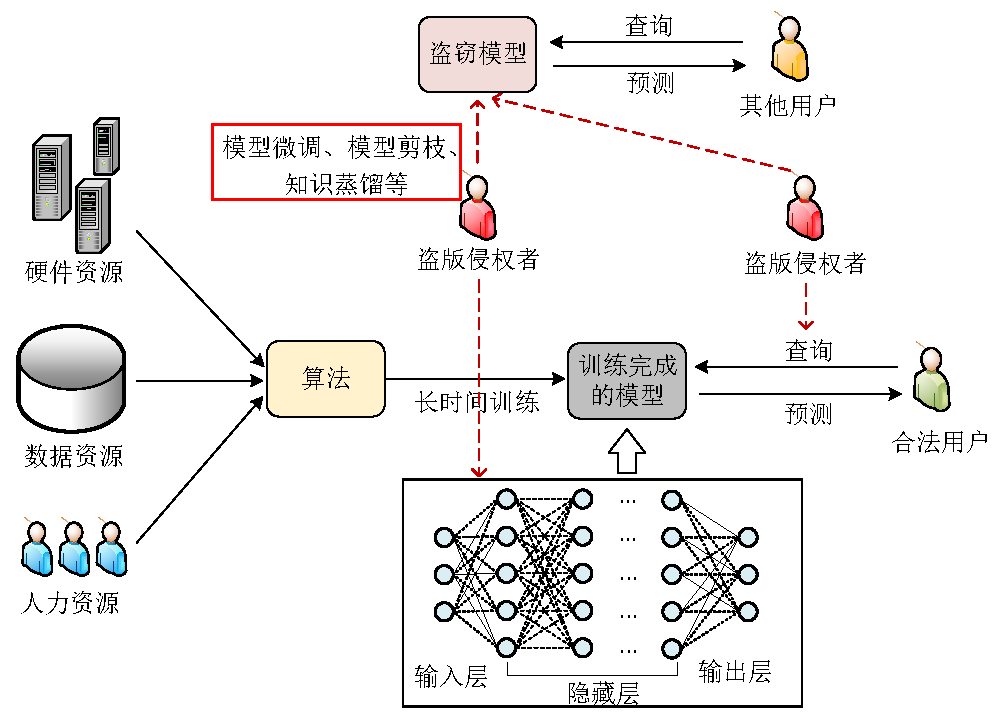
\includegraphics[width=0.97\linewidth]{DNN模型服务和盗窃示意图.pdf}
	\caption{DNN模型服务和盗窃示意图}
	\label{DNN模型服务和盗窃示意图}
%	\vspace{-3mm}  %调整图片标题与下文距离,与\setlength{\belowcaptionskip}{-3mm}等效。
	\end {figure}
	
如图\ref{DNN模型服务和盗窃示意图}所示,模型所有者消耗包括硬件资源、数据资源、人力资源在内的大量资源,经复杂算法进行长时间训练后,发布训练好的模型为合法用户提供服务。然而,盗版侵权者会对模型发起窃取攻击,从而获得一个功能相似的盗窃模型用于自己盈利。主要有两种方式:(1)直接访问原始模型,盗窃后对模型进行修改。(2)在不能直接访问模型时,通过模型提供的服务API进行特定的输入查询,依靠API输出重构模型。

\textbf{模型盗窃方法:}图\ref{DNN模型服务和盗窃示意图}中,不法分子可以通过模型窃取攻击来盗窃模型。主流的模型窃取攻击涉及到对模型的修改,主要包括模型微调\cite{guo2019spottune},模型剪枝\cite{liu2018rethinking},模型压缩\cite{deng2020model}等,简要介绍如下:

1)模型微调:型微调通常用于迁移学习,可以在原始模型的基础上微调模型参数,使模型满足自己的任务需求,同时保持模型的性能。通过微调现有的模型,可以派生出许多功能、结构相似的模型。

2)模型剪枝:模型剪枝是是部署DNN模型的常见方法之一,通过参数修剪来减少DNN的内存需求和计算开销,以便部署到一些资源受限的环境下。然后而模型盗窃者可能会使用修剪来删除水印或指纹。

3)知识蒸馏:模型压缩中常见的方式是知识蒸馏\cite{gou2021knowledge},可以将训练好的模型的知识,蒸馏到其他模型上。这种方式可以更快的训练一个新模型,显著降低模型的训练成本,内存需求和计算开销,同时达到与原始模型接近的性能。研究\cite{hinton2015distilling}表明甚至不需要原始训练数据就可以直接利用API蒸馏模型,因此蒸馏常被用来派生模型。
	
综上所述,如何在训练和部署时保护深度神经网络模型的知识产权是AI领域亟待解决的问题。保护DNN模型知识产权的意义在于确保模型的创造者能够获得其所创造的价值,具体而言,有以下四个方面的意义:

1)保护商业利益:神经网络模型模型通常需要大量的时间、资源和资金才能进行开发和训练。通过保护知识产权,模型的创造者可以确保他们的商业利益得到保护,从而获得他们应得的经济回报。

2)保护创新:神经网络模型模型是创新的产物,保护模型知识产权可以激励更多的人投入到相关研究和开发中。这样可以催生更多的创新,从而推动技术的进步和发展。

3)避免盗用和侵权:保护知识产权可以避免其他人对神经网络模型的盗用和侵权。这些行为可能会导致模型的创造者无法获得应有的经济回报,并可能削弱创造者的商业利益。

4)确保模型质量:通过保护知识产权,模型的创造者可以控制和保证其模型质量。这样可以确保DNN模型在商业应用中的可靠性和有效性,从而提高其商业价值和应用性。


\section{相关研究现状}

神经网络模型作为数字产品,不仅是设计者的知识智慧的结晶,还需要消耗昂贵的计算资源、花费大量的训练时间和海量的训练数据做支撑。近年来,先进模型所带来的工业优势已经被广泛认可,但这也引发了一些不法分子对这些模型进行攻击和窃取。神经网路模型将在未来的信息技术发展中扮演核心角色,因此保护这些模型的重要性显得更加突出。1994年,Van Schyndel等人\cite{van1994digital}首次提出了数字水印的概念,通过将标记隐蔽的嵌入到如音频、视频等数字内容中,来识别其所有权。具体而言,版权所有者通过显示此类标记的存在可以证明其对内容的所有权。由于DNN模型也是一种数字产品,因此,许多研究者从数字媒体水印得到启发,从而设计模型水印和模型指纹用于解决模型的所有权问题。
%\vspace{-3mm}

\subsection{模型水印}

模型水印\cite{GYKJ202207020}是解决神经网络模型知识产权问题的主要方式之一,Uchida等人\cite{uchida2017embedding}在2017年首次提出了在模型中嵌入水印的通用框架。该方法是一种白盒的模式,通过在训练时使用正则化器,这种正则化在参数中引入了所需要的统计偏差来作为嵌入的水印。模型所有者清楚模型内部结构等的细节,并且可以提取嵌入的水印,以此来作为验证模型所有权的依据\cite{zhang2021deep}。Fan等人\cite{fan2019rethinking}提出了一种在模型中嵌入数字护照的方案,嵌入数字护照的要点是设计和训练DNN模型,使得在伪造护照的情况下,神经网络模型的推断性能显著下降,而真正的护照可以通过查找预定签名来验证。Chen等人\cite{chen2018deepmarks}提出了一种新颖的端到端框架,该框架同时依赖于用户和模型,它需要为每一个用户分配一个代码向量,并将该信息嵌入到可训练权重的的概率密度函数中,同时保持模型的准确性。不同于白盒的模式,另一种黑盒的模式,可以在不访问模型内部的情况下,通过特定的输入输出来验证模型的所有权。Le等人\cite{le2020adversarial}提出了一种零比特水印算法,该算法标记模型的操作本身,稍微调整它的决策边界,来使特定的查询得到特定的输出。在减少模型性能损失的同时,该算法可以远程操作模型或API服务,通过少量的查询提取水印。Zhang等人\cite{zhang2018protecting}提出了一种水印植入方法,将水印注入模型。通过扩展神经网络的内在泛化和记忆能力,使得模型能够在训练时学习特意制作的水印,然后在推断时激活预先指定的预测。Adi等人\cite{adi2018turning}提出了利用模型的后门机制当作DNN模型水印。后门通常是指神经网络模型将输入预测为错误的标签,虽然在大多数情况下这是不可取的,但是却可以将为DNN模型制作水印的任务转化为设计后门的任务。这些黑盒的方法利用对抗性样本作为触发集,或者使用一组特定的训练样本,然后根据特殊样本的输出来提取水印。因此黑盒的方法在所有权验证中不需要访问模型的权重参数和内部结构。Rouhani等人\cite{rouhani2018deepsigns}提出了一种端到端的IP保护框架DeepSigns,可以在DNN模型中插入连贯的数字水印。DeepSigns引入了一种通用水印方法,不同于直接将水印信息嵌入到模型的权重中,DeepSigns将任意N位字符串嵌入到各层激活集的概率密度函数中,这意味着水印信息嵌入在DNN的动态内容中,并且只能通过特定的输入数据来触发,并且对权重矩阵等静态属性没有影响。

然而,DNN模型水印的嵌入步骤总是会对原始模型进行修改。具体而言,白盒水印修改模型内部,比如模型权重、激活函数、甚至模型架构,而黑盒水印通过特殊的训练调整模型来指定特定的输出。这些修改将会影响DNN模型在原始任务上的性能。除了减少对模型性能的影响,如何减小模型水印的嵌入代价也是模型水印的重要目标。

\subsection{模型指纹}

模型指纹是解决神经网络模型知识产权问题的又一主流方法。不同于模型水印,模型指纹不需要对模型本身进行修改,而是利用模型本身来寻找和提取一些固有的的特征作为模型指纹,一般来说,不会影响模型的性能。

Zhao等人\cite{zhao2020afa}提出了一种针对神经网络分类模型的指纹技术,该技术旨在提取模型本身的固有特征,而不是嵌入额外的水印。具体而言,该方法选择一组专门设计的对抗性样本作为模型指纹特征,称为对抗性标记,相比于其他不相关的模型,它可以更好地从原始模型转移到派生出的模型上。与Zhao等人\cite{zhao2020afa}的方法类似,Lukas等人\cite{lukas2019deep}提出了一种用于神经网络分类器的指纹识别方法。该方法从源模型中提取一组特殊的输入,以便只有源模型的派生模型在此类输入的分类上与源模型一致。这些输入是可转移对抗性样本的一个子类,它们的目标标签会从源模型转移到其派生模型上。所有者通过验证分类是否一致,判断模型是否从源模型派生。Cao等人\cite{cao2021ipguard}针对DNN分类器提出了一种名叫IPGuard的指纹方法,该方法的关键是分类模型可以由其分类边界唯一的表示。基于这一原理,IPGuard在模型所有者的神经网络模型分类边界上提取了一些数据点,并使用它们对分类器进行指纹识别,如果DNN分类器对大多数指纹数据点预测相同的标签,那么该模型被认为是模型所有者分类器的盗版模型。Li等人\cite{li2021novel}提出了一种适用于生成对抗网络(Generative Adversarial Network, GAN)\cite{goodfellow2020generative}知识产权保护的指纹识别方案。该方案从目标GAN和分类器构建了一个复合深度学习模型,然后从该复合模型中生成隐蔽的指纹样本,并将其注册到分类器中进行有效的所有权验证。Dong等人\cite{dong2021fingerprinting}针对模型水印和指纹容易受到最抗性训练攻击,不适用于多出口DNN模型的知识产权验证的问题,提出了一种根据推理时间,而不是推理预测的结果来为多出口模型建立指纹的新方法。

然而,模型窃取攻击通常会涉及到对原始模型的修改,作为指纹的固有特征也会受到影响。因此指纹是脆弱的,所有的指纹方法都试图找到可以承受某些修改攻击的强鲁棒性指纹。此外,模型指纹不适用于小样本数据集。对于小样本数据集,由于模型的特征向量可能会存在过拟合或欠拟合的情况,因此可能会导致模型指纹的准确性降低。

\textbf{歧义攻击问题:}虽然模型水印和模型指纹在保护模型知识产权方面已经取得了很大的进展,但除了上述提到的问题外,无论是水印还是指纹都容易受到歧义攻击\cite{fan2019rethinking,li2019piracy}。歧义攻击是指不法分子盗窃模型后,通过为神经网络模型伪造其他水印或指纹来对所有权验证产生干扰。直觉上,如果模型盗窃者可以在水印模型上嵌入第二个水印或者提取第二个指纹,那么该模型的所有权归属存在巨大的歧义。


\section{本文主要工作}

为了解决深度神经网络模型的知识产权问题,本文提出了近边界数据,一种分布在分类边界附近的特殊样本。模型指纹\cite{cao2021ipguard}使用对抗性样本抽象地反映模型分类边界,同一组对抗性样本的输入,其引起的决策模式的变化可以用于比较模型知识的相似性。但是这种方法是脆弱的,对模型的任意操作都有可能破坏这种特性。因此,本文不直接比较决策模式的变化,它是不可信任的,而是比较对抗性样本与分类边界的距离。大多数对抗性样本都是位于分类边界附近的,也就是说,它们与分类边界的距离很近。对抗性样本的这种性质被本文所利用并构造近边界数据。经过测试,本文发现绝大多数的模型窃取方法都无法改变这种结果,即使在盗窃模型中样本分类受到影响,其仍然位于分类边界附近。近边界数据背后的意义是如果被用于所有权验证如果两个模型的决策模式相似,参与训练的近边界数据一定可以反映出来。受这个特性的启发,将近边界数据作为水印验证所有权是传统的思路,即使不会对模型的精度造成影响,这样的水印也是脆弱的,很难抵御歧义攻击。因此本文提出由近边界数据驱动的模型所有权推断方法,代替传统的模型水印、指纹验证所有权。

本文方法的主要原理如图\ref{方法原理图}所示,其思想是构造私有的近边界数据,当判断一个模型的所有权时,模型所有者和盗窃者分别提供各自的私有近边界数据,距离分类边界最近的被推断获得所有权。

\begin{figure}[htb]%%图,[htbp]是浮动格式
	\centering
	\setlength{\abovecaptionskip}{5mm} %图片标题与图片距离
	%	\vspace{-2mm}
%	\setlength{\belowcaptionskip}{-3mm} %调整图片标题与下文距离
	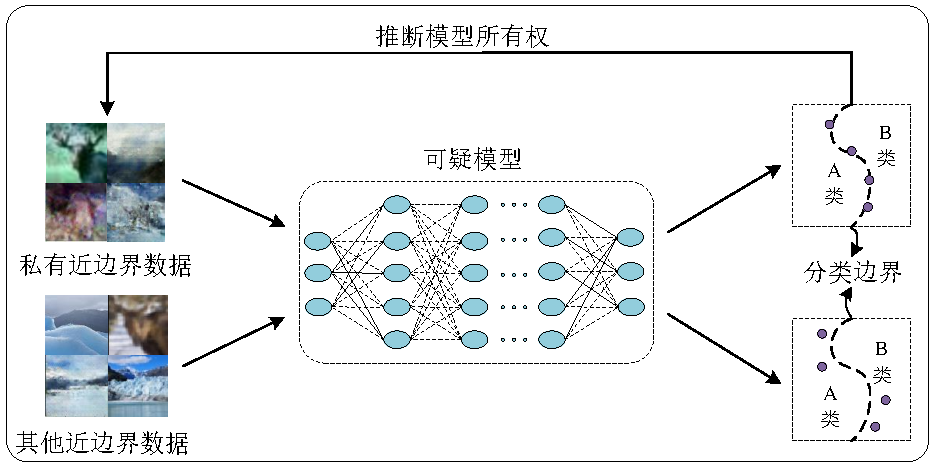
\includegraphics[width=1\linewidth]{方法原理图.pdf}
	\caption{近边界数据推断所有权}
	\label{方法原理图}
	%	\vspace{-3mm}  %调整图片标题与下文距离,与\setlength{\belowcaptionskip}{-3mm}等效。
	\end {figure}

本文的主要工作如下:

1)提出基于数据推断模型所有权的新思路,并利用对抗性样本构造近边界数据以抵御模型窃取攻击。与过去工作中利用模型水印和指纹验证模型所有权相比,使用数据在对应模型上结果作为所有权推断依据,结果的可比性和唯一性可以有效避免歧义攻击。通过实验验证了近边界数据的近边界性可以很好的继承到从源模型派生出的模型上,因此可以作为推断模型所有权的依据。本文利用生成对抗性样本算法生成了初始近边界数据。

2)设计了基于DCGAN的近边界数据特征提取器,用以私有化初始的近边界数据,并且设计了一种新的损失函数用以微调源模型,增加推断模型所有权的置信度。为了防止近边界数据被轻易伪造,本文训练了DCGAN作为数据特征提取器,提取近边界数据特征后,生成新的、私有化的近边界数据。在此基础之上,重新设计了新的损失函数微调源模型,在保持DNN模型性能的情况下,以95\%以上的置信度成功推断模型所有权。

3)基于ResNet18\cite{he2016deep}和三个公开数据集进行了广泛的实验,实验结果证明了近边界数据在推断模型所有权上的显著效果。本文在三个公开数据集上分别训练了ResNet18作为源模型,并且使用模型微调,不同比例模型剪枝,知识蒸馏几种方式派生出盗窃模型,使用VGG11\cite{simonyan2014very}作为无关对照模型。对生成初始近边界数据的方法选择、近边界数据私有化方法的选择、近边界数据的可继承性、源模型微调的影响、模型所有权推断的有效性和近边界数据规模的可伸缩性几个方面对本文提出的方法进行了详细的实验和分析,实验结果证明了基于近边界数据推断模型所有权方法的有效性和鲁棒性。

\section{本文组织架构}

\begin{figure}[htb]%%图,[htbp]是浮动格式
	\centering
		\setlength{\abovecaptionskip}{5mm} %图片标题与图片距离
%	\vspace{-2mm}
%	\setlength{\belowcaptionskip}{-3mm} %调整图片标题与下文距离
	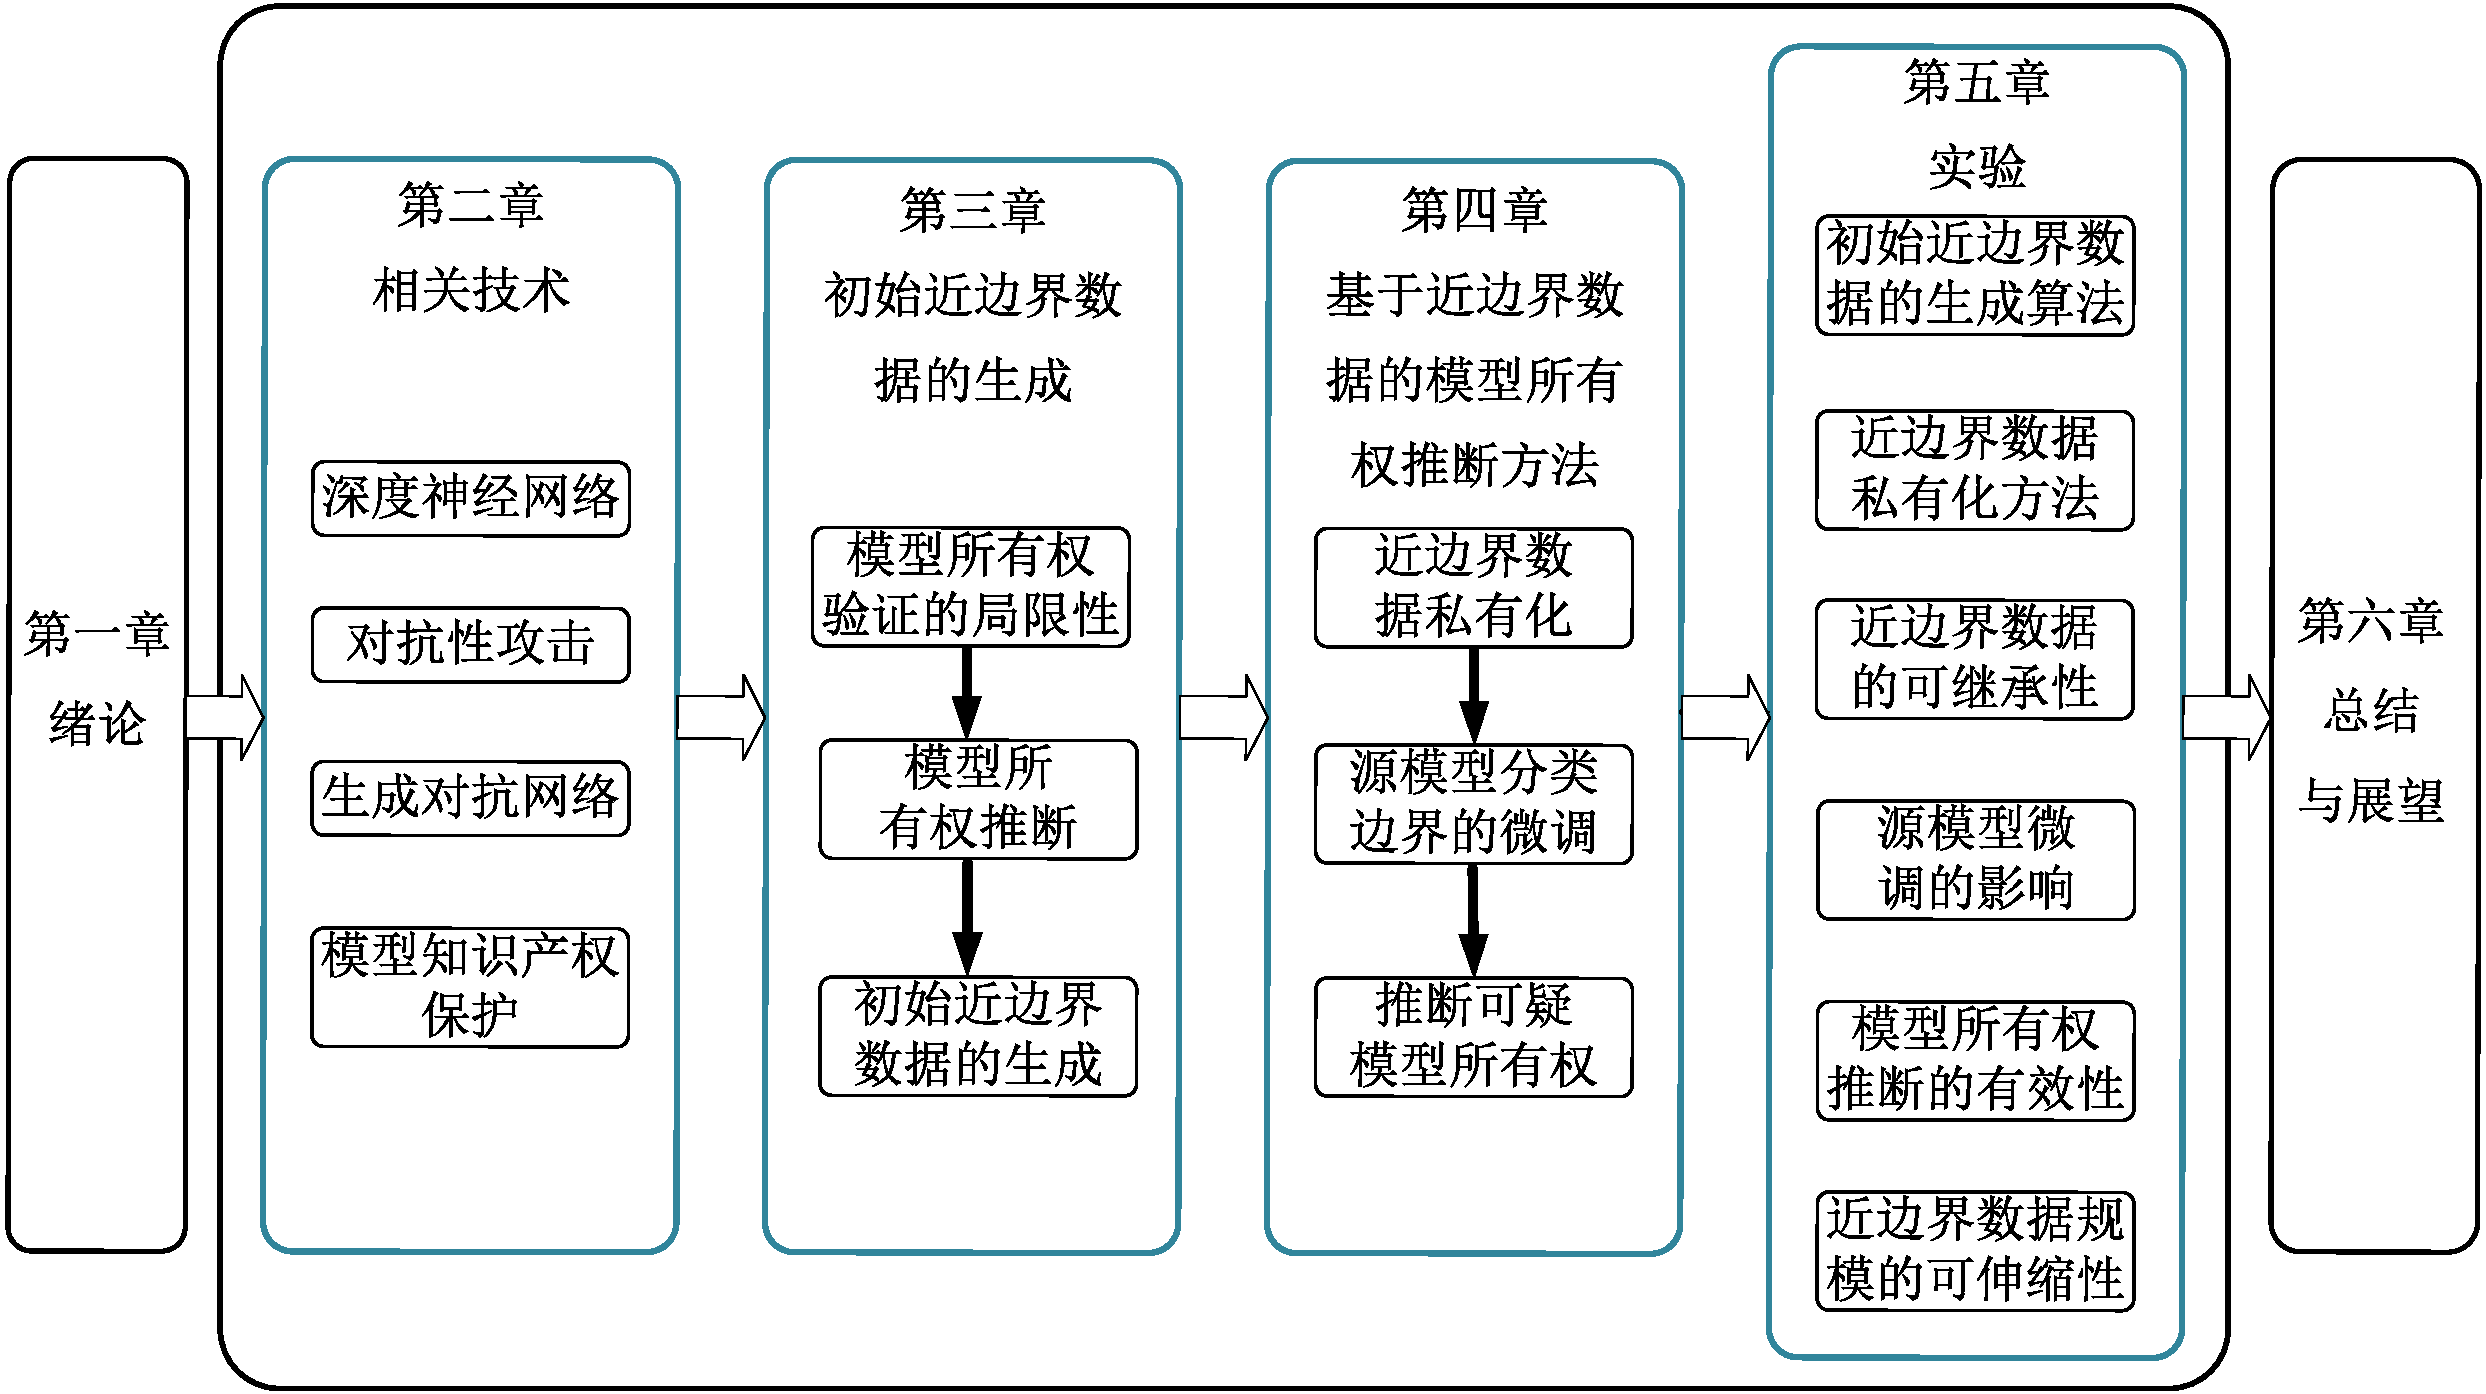
\includegraphics[width=1\linewidth]{章节架构图.pdf}
	\caption{章节架构图}
	\label{章节架构图}
	%	\vspace{-3mm}  %调整图片标题与下文距离,与\setlength{\belowcaptionskip}{-3mm}等效。
	\end {figure}
	
本文对近边界数据进行研究,提出一种基于近边界数据推断模型所有权的方法。本文的组织架构如图\ref{章节架构图}所示,第二章为后面章节提供技术基础。第三章提出模型所有权推断代替所有权验证,解决歧义攻击问题,并生成所有权推断所需的初始近边界数据。第四章在第三章的基础上对初始近边界数据进行初始化,然后基于近边界数据进行所有权推断。第五章对本文提出方法进行全面的测试与评估。全文共分为六各章节,每个章节的主要内容如下:

第一章:绪论。本章首先介绍了神经网络模型在当今时代的广泛应用和研发的昂贵成本,说明了保护DNN模型知识产权的必要性和重大意义,然后介绍了模型水印和模型指纹两种保护方法的研究现状,并针对相关研究存在的问题提出了本文的研究内容,最后简要说明了各个章节的内容安排。

第二章:相关技术。本章首先介绍了深度神经网络基本原理和结构并解释本文使用到的相关术语,然后介绍了对抗性攻击和生成对抗网络的基本原理,最后介绍了模型水印、模型指纹两种知识产权保护方法。为第三章、第四章提供技术基础和理论依据。

第三章:初始近边界数据的生成。本章首先分析了通过传统模型水印、模型指纹来做所有权验证的局限性,然后提出了数据驱动的所有权推断方法。接着研究了近边界数据在源模型和其派生模型上的可继承性,说明近边界数据可用于所有权推断。最后生成了所有权推断所需的初始近边界数据。

第四章:基于近边界数据的模型所有权推断方法。本章首先介绍了需要将初始近边界数据私有化的原因,然后训练生成对抗网络,用其生成器生成新的、私有化的近边界数据。然后设计了新的损失函数微调源模型,使私有近边界数据更加靠近目标分类边界,增加成功推断模型所有权的置信度。最后提出使用假设检验的方法来统计对比结果差异。

第五章:基于近边界数据的模型所有权推断方法分析。本章在ResNet18和三个公开数据集上,对生成初始近边界数据的方法选择、近边界数据私有化方法的选择、近边界数据的可继承性、源模型微调的影响、模型所有权推断的有效性和近边界数据规模的可伸缩性几个方面进行了详细的实验和评估,证明了本文提出方法在推断模型所有权时的有效性和鲁棒性。

第六章:总结与展望。本章总结了全文的工作,分析了本文提出方法在解决模型知识产权问题时的优势与不足,并针对不足之处,提出了未来研究工作的改进方向。

% !TeX root = ../main.tex
% -*- coding: utf-8 -*-


\chapter{相关技术} \label{2}

本章主要介绍深度神经网络模型知识产权领域的相关技术。首先,介绍了深度神经网络的基本结构和原理以及本文涉及到的相关术语,便于理解本文提出的方法。然后,着重介绍了对抗性攻击和生成对抗网络的原理,为近边界数据的生成提供技术基础。最后,介绍模型水印和指纹两种主流知识产权保护方法的原理和实现方式。

\section{深度神经网络}

人工神经网络是一种模拟生物神经系统的信息处理模型,旨在通过一系列相互连接的神经元(网络中的节点)来处理复杂的数据。它可以被看作是由许多基本单元组成的网络,每个基本单元都可以接收来自其他基本单元的信号并输出一个新的信号。通常,神经网络由输入层,隐藏层和输出层组成。如图\ref{深度神经网络结构图}所示,如果神经网络有多个隐藏层,则被称为深度神经网络。深度神经网络的隐藏层一般由多个卷积层,池化层,全连接层,Dropout层和Softmax层构成,这些层能够提取数据的高级特征,并对复杂的非线性数据进行有效建模。在神经网络的训练过程中,数据输入到输入层,通过每一层后,每层会提取出一些抽象特征作为下一层的输入,最终由输出层输出最终结果。
	
\begin{figure}[htbp]%%图,[htbp]是浮动格式
	\centering
	\setlength{\abovecaptionskip}{3mm} %图片标题与图片距离
%	\vspace{-2mm}
	\setlength{\belowcaptionskip}{-3mm} %调整图片标题与下文距离
	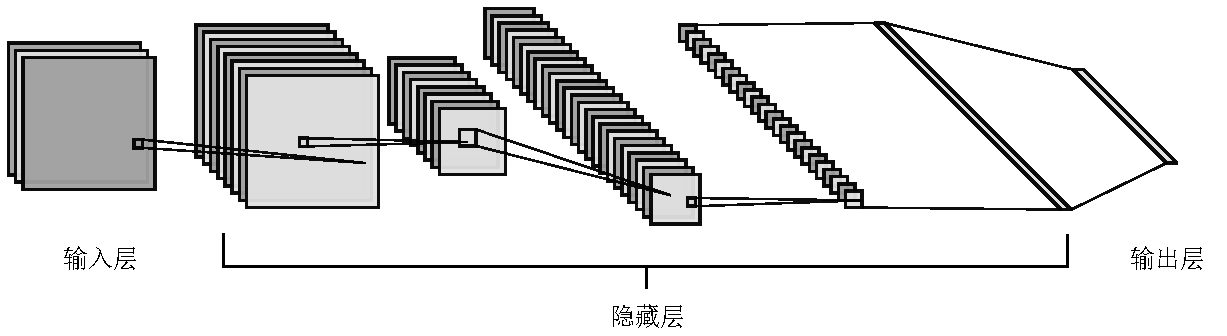
\includegraphics[width=1\linewidth]{深度神经网络结构.pdf}
	\caption{深度神经网络结构图}
	\label{深度神经网络结构图}
	%	\vspace{-3mm}  %调整图片标题与下文距离,与\setlength{\belowcaptionskip}{-3mm}等效。
	\end {figure}

深度神经网络一种非常强大的非线性数学函数,能够将一组输入变量转化为一组输出变量。每个神经元都有对应的权重和偏置参数,这些参数控制着输入的精确转化,从而实现了高度准确的数据建模和预测。在DNN模型的训练过程中,需要确定神经网络中每个神经元的权重和偏置参数。这个过程可以通过梯度下降算法和反向传播来实现。梯度下降算法通过最小化损失函数来更新参数,反向传播则是用来计算参数的梯度,从而实现参数的更新。神经网络模型的学习和训练是一个需要大量计算资源的过程,然而一旦权重和偏置参数确定,DNN模型就可以快速地处理相似类型的新数据,识别并提取海量数据中的复杂特征。

以下是本文中涉及到的\textbf{相关术语}:

1)源模型。源模型也称作目标模型、原始模型,是指模型所有者在私有或公开数据集上,消耗大量计算资源和人力资源训练出的高性能DNN模型,可能因学术研究放置在开源社区,或者作为商用给用户提供远程API。

2)可疑模型。可疑模型也称作盗窃模型、替代模型、派生模型,是指该模型可能是通过模型窃取攻击方法从源模型派生的模型,判断一个可疑模型是否是从源模型派生是模型知识产权保护领域的主要目标。

3)白盒环境。白盒环境是指能够获得DNN模型的所有知识,包括训练集,训练方式,模型参数,模型结构等。

4)黑盒环境。黑盒环境指不清楚模型内部参数和结构等,但可以通过模型提供的API获得指定输入的输出。

5)\textbf{验证模型所有权}。验证模型所有权指通过检测有无特定的水印或者指纹是否匹配的方式解决模型的所有权问题,检测到特定的水印或者指纹匹配说明验证所有权成功。

6)\textbf{推断模型所有权}。推断模型所有权是本文提出的新概念,指通过数据在模型上的最优性解决模型的所有权问题,最优数据提供者推断获得所有权。




\section{对抗性攻击}

\subsection{对抗性样本}
 
对抗性样本的概念是Szegedy等人\cite{szegedy2013intriguing}提出的。这篇文章中指出,通常情况下,一个性能良好的神经网路模型具备优异的泛化能力,即对输入的微小随机扰动具较强有鲁棒性,从而保证了模型在处理图像时的类别预测准确性。然而,如果对图像添加特定的非随机扰动,使得损失函数的值上升,那么DNN模型的预测结果就可以随意改变。这些难以被人眼察觉但足以使得模型输出错误类别的图像样本即为对抗性样本。

\begin{figure}[htbp]%%图,[htbp]是浮动格式
	\centering
	\setlength{\abovecaptionskip}{3mm} %图片标题与图片距离
	%	\vspace{-2mm}
	\setlength{\belowcaptionskip}{-3mm} %调整图片标题与下文距离
	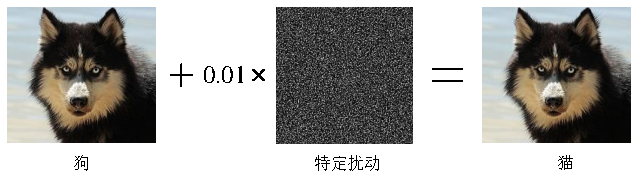
\includegraphics[width=0.9\linewidth]{对抗攻击示意图.pdf}
	\caption{对抗性攻击示意图}
	\label{对抗性攻击示意图}
	%	\vspace{-3mm}  %调整图片标题与下文距离,与\setlength{\belowcaptionskip}{-3mm}等效。
	\end {figure}

如图\ref{对抗性攻击示意图}所示,狗的图像被添加特定扰动后被分类器识别为猫。添加特定的扰动,甚至可以使模型输出任意类别。

\noindent\textbf{(1) \  黑盒场景   }

用$f:R^m \rightarrow {1,2,...,n}$表示将一张图片映射为$n$个标签的DNN分类器,对一个正常样本$x \in R^m$以及一个错误标签$l$,目标是找到一个最小的扰动$\delta$,使得分类器将样本$x$错误分类为$l$,如式\ref{eq:1}所示:
\begin{equation}
	\label{eq:1}
	\begin{split}
	min&\parallel \delta \parallel_2, \\
	 s.t. \ f(x + \delta) &= l,\ x + \delta \in [0,1]^m
	\end{split}
\end{equation}

其中叠加了扰动的$x+\delta$即为一个对抗性样本。式\ref{eq:1}这种方式通常用于黑盒的场景下,仅根据DNN分类器的输出进行扰动$\delta$的调整。
 
\noindent\textbf{(2)\  白盒场景   }
 
 在白盒场景下,由于知道模型的所有知识,可以根据这些信息来寻找对抗性样本,通常利用DNN分类器的损失函数来寻找对抗性样本。
 
 用$f:R^m \rightarrow {1,2,...,n}$表示将一张图片映射为$n$个标签的DNN分类器,对一个正常样本$x \in R^m$以及它对应的正确标签$y$,目标是找到一个足够小的扰动$\delta:\delta \leq \gamma$,使得加上扰动后的样本输入DNN模型后,损失函数$L$达到最大值,如式\ref{eq:2}所示:
 \begin{equation}
% 	\setlength\abovedisplayshortskip{1mm}
% 	\setlength\belowdisplayshortskip{4mm}
 	\label{eq:2}
 		\delta = arg \mathop{max} \limits_{\delta \leq \gamma} L(f(\theta, x + \delta), y)
% 		\vspace{3mm}
\end{equation}
%\vspace{-16mm}

其中$\theta$是分类器$f$的参数,$x + \delta$是一个扰动后的对抗性样本。
 
 \subsection{对抗性攻击的类别}

对抗性攻击技术是指生成对抗性样本的方法,不同的方法生成对抗性样本的效率,质量也不相同。根据方式的不同,可以分为以下几类:

1)白盒攻击与黑盒攻击。白盒攻击指敌手知道DNN模型的参数和内部结构等信息,利用这些信息发起的攻击。黑盒攻击指敌手仅根据模型的输入输出来发起攻击。

2)有目标攻击和无目标攻击。有目标攻击指对抗性样本的预测类别为敌手指定的类别,例如将一张牛的图片识别为羊,而不能是其他类别,常采取的方式是向各个方向搜索扰动来最大化DNN模型预测特定类上的可能性。无目标攻击指添加扰动来改变原始预测类别,对具体分类类别不做要求。通常来说有两种攻击方式,一种是最小化DNN模型预测正确类的可能性,一种是进行多次不同类别的的有目标攻击,然后在多个对抗性样本中选取扰动最小的。
	
3)单步攻击和迭代攻击。单步攻击指通过一次添加扰动生成对抗性样本,迭代攻击指通过多次迭代添加微小扰动来生成对抗性样本。通常来说迭代攻击的成功率较高,但是相应的算法复杂度更高,效率较低。
	
4)个体攻击和普适性攻击。个体攻击指针对每个样本都需要重新生成扰动,普适性攻击指找到一个通用的扰动,对数据集中的一类数据都叠加该扰动,普适性攻击效率较高,但是寻找通用扰动的难度较大。

\section{生成对抗网络}\label{2.3}

Goodfellow等人\cite{goodfellow2014generative}第一次提出了生成对抗网络(Generative Adversarial Network, GAN),是一种利用生成模型实现无监督学习的特殊方法。该网络由一个生成器和一个判别器组成,并通过一种相互博弈的方式进行训练。如图\ref{生成对抗网络结构图}所示,首先随机噪声作为生成器的输入,经过生成器转化成和真实图片具有相同维度的图像。使用原始图片和生成图片分别输入到判定器中,训练判定器区分它们的能力。接着,再使用真实图片训练生成器,使之生成的图片尽可能接近真实图片。通过迭代的交替训练,在训练收敛时,最终生成器生成的图片和原始图片在空间分布上基本一致,判定器判定生成图片和原始图片为真的概率均为$1/2$,也就是无法区分生成图片和原始图片。这种相互博弈的过程可视为生成器和判别器之间的对抗,因此称为生成对抗网络。

\begin{figure}[htbp]%%图,[htbp]是浮动格式
	\centering
	\setlength{\abovecaptionskip}{3mm} %图片标题与图片距离
	%	\vspace{-2mm}
	\setlength{\belowcaptionskip}{-3mm} %调整图片标题与下文距离
	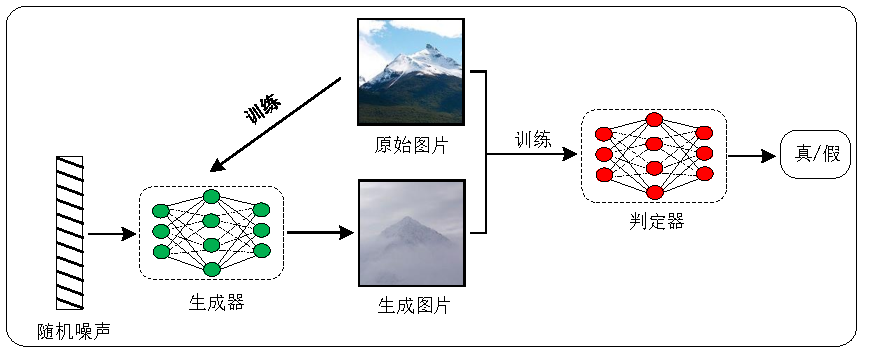
\includegraphics[width=0.97\linewidth]{生成对抗网络结构.pdf}
	\caption{生成对抗网络结构图}
	\label{生成对抗网络结构图}
	%	\vspace{-3mm}  %调整图片标题与下文距离,与\setlength{\belowcaptionskip}{-3mm}等效。
	\end {figure}

具体而言,生成器$G$和判别器$D$可视为博弈中的双方,当训练GAN模型时,生成器$G$和判别器$D$通过更新各自的参数使损失达到最小,经过不断迭代优化,最后$G$和$D$达到纳什均衡。GAN的目标函数如式\ref{eq:3}所示,对于原始图片$x$,判别器希望$D(x)$变大,对应于式中的$maxD$,对于生成图片$G(T)$,生成器希望$D(G(T))$变大,即$log(1 - D(G(T))$变小,对应于式中的$minG$,所以GAN的目标函数由两个目标构成。
\begin{equation}
	\label{eq:3}
	\begin{split}
		\mathop{min} \limits_{G} \mathop{max} \limits_{D} V(D, G) &= \mathop{min} \limits_{G} \mathop{max} \limits_{D} E_{x \sim P_{data}(x)}[logD(x)] \\
		&+ E_{T \sim P_{T}(T)}[log(1 - D(G(T)))]
	\end{split}
\end{equation}

其中$x$表示原始图片,$T$表示用于生成样本的随机噪声,GAN对噪声$T$的分布没有特别要求,常用的有高斯分布、均匀分布等,E表示数学期望。

在图像生成领域,生成对抗网络已被广泛应用于多种任务\cite{chen2022generative,singh2021medical,zhou2023hybrid},包括图像合成、图像修复、风格转换和图像生成等。由于GAN独特的训练方式,使其不仅仅在生成新图像方面表现出色,还可以用于图像特征提取\cite{xu2022te}。通过对原始图像进行特征提取,GAN的生成器可以生成与原始图像特征分布类似的新图片。这种方法已被成功应用于多个领域,例如医学成像和计算机视觉。因此,生成对抗网络在图像生成和特征提取方面的广泛应用将在未来的研究中得到进一步的探索和发展。

%%\section{模型窃取攻击}
%
%自DNN在各个领域取得巨大成功以来,针对DNN模型的攻击就层出不穷,按照攻击方式的不同,可以分为以下三类\cite{xue2021intellectual}:
%(1)模型修改攻击。指常见的模型修改,主要包括包括模型微调,模型剪枝,模型压缩,模型再训练等方式。
%(2)删除攻击。指攻击者试图逃避水印或指纹的检测,主要包括删除攻击,篡改攻击,逆向工程攻击等方式。
%(3)主动攻击。指攻击者主动攻击和强攻击,主要包括歧义攻击,水印和指纹覆盖攻击,查询修改攻击等方式。
%
%\subsection{模型修改攻击}
%
%模型盗窃者在盗窃DNN模型后,通常会对DNN模型进行修改或者压缩,然后部署模型作为MLaas来非法盈利。模型修改主要包括:
%
%1)模型微调。微调通常用于迁移学习中,包括在源模型的基础上,根据自己定制的任务,继续训练模型,使得DNN模型在保持性能的同时修改内部的参数。模型微调可以从源模型派生出非常多的模型。由于内部参数发生改变,水印等可能也会随之变化,因此这对水印的鲁棒性是一个考验。
%	
%2)模型剪枝。由于DNN模型通常内存占用多,计算开销大,因此模型剪枝是在小型设备上部署DNN模型的常用方法。但是模型盗窃者可能会利用剪枝来删除水印,因此有效的水印技术应该能够抵御由模型剪枝引起的参数变化。
%	
%3)模型压缩。模型压缩可以显著降低DNN模型的内存需求和计算开销,常用的方法是知识蒸馏,通过将大型模型包含的知识转移到小模型上来达到模型压缩的目的。
%	
%4)模型再训练\cite{namba2019robust}。模型再训练是一种很直接的方法,这样能尽可能的去除或者减少原有水印的影响,相应的,这种攻击方式成本也比较高。
%
%
%\subsection{删除攻击}
%
%目前大部分DNN模型的知识产权保护工作专注于水印对DNN模型被修改时的鲁棒性,而很少考虑水印或指纹本身受到的攻击。删除攻击主要包括:
%
%1)删除攻击\cite{shafieinejad2021robustness}。攻击者试图修改模型以删除原有的水印。
%
%2)篡改攻击。攻击者知道DNN模型中存在水印,试图窜改模型来删除原有的水印和指纹特征。
%
%3)逆向工程攻击\cite{fan2019rethinking}。如果攻击者知道并可以获得原始训练数据,可能会直接对内部参数进行逆向工程。
%
%
%Shafieinejad等人\cite{shafieinejad2021robustness}研究了DNN中基于后门的水印方法的移除攻击,表明攻击者可以仅依靠公共数据集删除水印,而不用访问训练集和模型参数。还提出了一种检验水印的方法,表明基于后门的水印不够安全,无法保持水印的隐藏。
%
%
%\subsection{主动攻击}
%
%除了被动的攻击方式,攻击者还可能对DNN模型发动更强的主动攻击。主动攻击主要包括:
%
%1)歧义攻击。歧义攻击指在DNN模型上伪造额外的水印来混淆所有权的验证。研究表明,除非采取不可逆的水印方案,否者即使是鲁棒性的水印,也不一定能验证模型的所有权\cite{fan2019rethinking}。
%
%2)水印覆盖攻击\cite{darvish2019deepsigns, chen2019blackmarks, chen2019deepmarks}。即使攻击者不知道具体的私有水印信息,但他知道模型水印嵌入的方法,就可能通过在DNN模型中嵌入新的水印来覆盖原有的水印,从未破坏原有的水印使其不可读。
%
%3)查询修改攻击。攻击者修改查询结果来使得水印验证过程无效。一个典型的方式是攻击者获得DNN模型并部署为MLaaS后,会主动检测一个查询是否为水印验证查询,从而修改或者屏蔽该查询,使水印验证无效。



\section{模型知识产权保护}

为了训练一个高性能的神经网络模型,需要该领域专家的先验知识来设计模型结构,大量的训练数据、昂贵的计算资源和漫长的训练时间。因此,训练后的DNN模型属于模型所有者的知识产权。由于DNN模型在各个领域都得到了高效的应用,许多不法分子开始盗窃、复制和修改这些模型以获利。为了保护神经网络模型的知识产权\cite{JFYZ202205002,WXAQ202202001},许多学者受多媒体数字水印的启发,使用模型水印和模型指纹来验证DNN模型的所有权。

\subsection{模型水印}

模型水印是第一种被提出的保护DNN模型知识产权的方法,根据水印嵌入方式和提取方式的不同,主要分为白盒水印和黑盒水印。

\noindent\textbf{(1) \  白盒水印   }

在白盒场景下,模型所有者可以利用模型的全部知识构造水印,这些知识包括训练数据集,训练方法,模型内部权重参数和结构。Kuribayashi等人\cite{kuribayashi2020deepwatermark}提出一种可量化的水印嵌入方法,该方法基于全连接层的权重,为了使嵌入水印不对模型造成太大影响,通过改变训练中的参数来量化水印的影响。不同于基于权重的方法,基于内部结构的水印方法抵抗模型修改的鲁棒性更强。在DNN模型中,可以改变模型的结构,添加额外的一层作为护照\cite{fan2019rethinking},以此来作为数字签名,增加模型的安全性。当不法分子发起歧义攻击,尝试嵌入额外水印时,模型性能会急剧下降。然而,这种方式的部署代价非常高。

\noindent\textbf{(2) \ 黑盒水印   }

在黑盒场景下,盗窃模型的内部结构和权重参数等是未知的,模型所有者只能通过其提供的API服务进行水印验证。一般而言,黑盒水印通过构造特殊的触发集实现,主要有以下几种方式:

1)通过更改样本标签构造触发集,将原始样本标签更改为模型所有者指定的与原始内容不符合的标签,这样仅修改标签不做任何其他修改的水印方法称为零位水印。

2)通过在原始样本中嵌入额外水印信息和更改标签构造触发集,这样可以在模型输出中嵌入模型所有者的版权信息。

3)通过添加新的样本构造触发集,这样的方式对模型的精度影响较大,一般通过模型微调最大限度的减少新样本对模型决策的影响。



\subsection{模型指纹}

模型指纹一般是利用模型本身来寻找和提取一些固有的特征来作为指纹。相较于模型水印的方法,模型指纹一般不对模型进行修改,因此不会影响模型的精度。一般来说,可以选择靠近决策边界的对抗性样本作为模型的指纹特征,来验证模型所有权。模型指纹分为指纹生成和指纹验证两个阶段。

\noindent\textbf{(1) \  模型指纹生成   }

指纹生成是模型指纹技术中的第一阶段,它需要选择一组样本来生成指纹。模型指纹与生物学上的指纹类似,具有唯一标识性,用以标记DNN模型的所有权。根据之前对指纹的相关研究\cite{zhao2020afa,lukas2019deep,cao2021ipguard},可以把靠近决策边界的对抗性样本作为模型的指纹。这些样本可以通过将一个已知标签的样本加上一些扰动来生成,从而欺骗模型产生错误的分类结果。具体来说,通过将此类样本输入DNN模型,将其对应的输出标签作为模型的指纹标签。

对于一个正常样本$x$,添加一个微小的扰动$\delta$,使得第$i$个输出满足:
\begin{equation}
	\label{eq:4}
	arg \mathop{max} \limits_i g_i(x) = y \wedge arg \mathop{max} \limits_i g_i(x + \delta) = y'
\end{equation}

其中$y$表示输入样本$x$对真实标签,叠加扰动后输出$y' \neq y$,$\delta$是对抗扰动,$x + \delta$即为对抗样本。

所以一组对抗性样本作为指纹样本,对应的输出作为指纹标签,共同构成模型指纹。即$X' = \{x_1',x_2',...,x_n'\}$作为模型指纹样本,对应的预测结果$Y' = \{y_1', y_2',...,y_n'\}$为指纹标签。\\

\noindent\textbf{(2) \ 模型指纹验证   }

指纹验证是模型指纹技术中的第二个阶段。在这个阶段中,生成的指纹将被用于验证模型的所有权。验证过程基于相同的原理,即使用对抗性样本来检查模型的响应。具体来说,在模型指纹验证阶段,通常的做法是使用指纹样本查询可疑模型API,比较API返回的预测标签和指纹标签的匹配程度。

设定一个阈值$\tau$,当阈值标签和指纹标签的匹配成功率超过阈值$\tau$时,则视为匹配成功,判定提供指纹样本的人是模型的合法拥有者。

设$X' = \{x_1',x_2',...,x_n'\}$为$n$个指纹样本,$Y' = \{y_1', y_2',...,y_n'\}$为对应的指纹标签,将$n$个指纹样本输入可疑模型API后,预测标签为$\widetilde{Y}' = \{\widetilde{y_1}', \widetilde{y_2}',...,\widetilde{y_n}'\}$。其中预测标签与指纹标签相同的数量为$q$,即$y_i' = \widetilde{y_i}'(i = 1, 2,...,q)$。

定义验证函数如下:
\begin{equation}
	\label{eq:5}
	Verify(Y', \widetilde{Y}')= \left
	\{ 
	\begin{array}{ll} 
		1, &\quad \dfrac{q}{n} \geq \tau \\ 
		\\
		0, &\quad \mbox{其他}\\ 
	\end{array} 
	\right.
\end{equation}

式\ref{eq:5}中,$q/n$表示匹配成功率,$\tau$是判定阈值。当匹配成功率大于等于阈值$\tau$时,结果为$1$,表示指纹成功匹配,判定可疑模型为盗版模型。


\section{本章小结}

本章主要介绍了深度神经网络,对抗性攻击,生成对抗网络和知识产权保护这四个方面的相关概念和理论基础。深度神经网络复杂的结构使其训练昂贵耗时,但是一旦训练完成就可以快速处理新数据。对抗性样本是一种人类肉眼无法察觉到变化而会导致模型输出错误的特殊样本,根据方式的不同,有多种生成的方法。本文利用对抗性样本靠近模型分类边界的特点构造初始近边界数据。生成对抗网络具有强大的特征提取能力,可以利用其生成与训练样本特征分布类似的新样本。本文生成对抗网络提取初始近边界数据的特征,然后使用生成器生成新的、私有的近边界数据。在神经网络模型知识产权保护领域,目前使用最广泛的是模型水印和指纹这两种方法,它们大多基于验证模型所有权的思路进行设计与实现。

% !TeX root = ../main.tex
% -*- coding: utf-8 -*-

\chapter{初始近边界数据的生成}\label{3}

目前,大多数模型的知识产权保护方法采用模型水印和模型指纹等被动防御方式来进行所有权验证,这种方式很难抵御歧义攻击。数据集推断利用训练数据在模型上的最优性进行所有权决策,从而验证所有权,但要求训练数据私有,因此应用范围小且推广难度高。因此,本文提出了一种数据驱动的推断模型所有权的新思路,该方法利用数据在模型上的最优性来推断模型所有权,代替传统的水印和指纹验证模型所有权,可以有效避免歧义攻击。同时,本文通过构造一种特殊的数据代替训练数据来推断模型所有权,使得训练数据可以被公开。

\section{模型所有权验证的局限性}\label{3.1}

现有的模型知识产权保护措施着重于被动的防御,只考虑针对模型修改的抗攻击性。模型所有者将水印嵌入训练好的模型或从其中提取抽象的模型知识作为指纹。如果怀疑一个模型的知识来自于源模型,模型所有者可以利用水印或指纹被动地从外部验证模型所有权,当检测到相应的水印或者指纹相匹配就代表该模型是从源模型派生。大多数工作基于这样的思路,设计不同的水印和指纹用于在源模型被盗窃后验证模型所有权,但这并不具备较强的鲁棒性。嵌入水印对源模型性能和功能的影响和需要的的额外代价都是模型水印研究工作的关键点。模型指纹目的是提取代表模型知识的固有特征,相较于水印指纹不会对源模型产生影响,因为模型的知识是容易被修改,因此指纹是脆弱的,所有的指纹方法都试图找到可以承受某些修改攻击的强鲁棒性指纹。

本文的目标不仅是抵御一般的模型窃取攻击,还集中在水印和指纹另一个亟待解决的问题歧义攻击上。歧义攻击不关心如何去除水印和指纹以通过模型所有权验证,而是通过伪造额外的水印和指纹混淆所有权验证。

如图\ref{歧义攻击示意图}所示,为了保护自己的知识产权,模型所有者在训练完源模型后,给DNN模型嵌入水印,然后发布模型提供公开服务。模型盗窃者访问公开的模型或者模型所提供的服务API,通过一定的方法复制篡改而得到盗版模型。为了躲避模型所有者的检测,盗窃者不关心原有的水印,而是给模型嵌入自己的额外水印。模型指纹的歧义攻击与水印类似,盗窃者不关注原有的指纹,而是提取新的指纹,以此混淆模型所有权的验证。

\begin{figure}[htb]%%图,[htbp]是浮动格式
	\centering
	%	\setlength{\abovecaptionskip}{2mm} %图片标题与图片距离
	\vspace{-2mm}
	\setlength{\belowcaptionskip}{-3mm} %调整图片标题与下文距离
	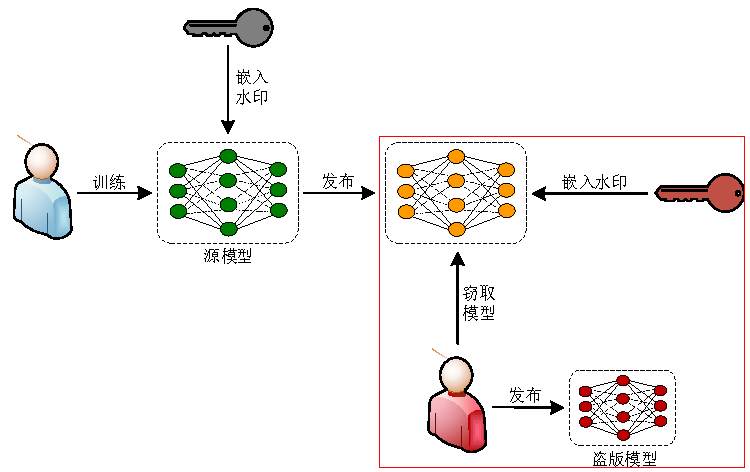
\includegraphics[width=0.9\linewidth]{歧义攻击示意图.pdf}
	\caption{歧义攻击示意图}
	\label{歧义攻击示意图}
	%	\vspace{-3mm}  %调整图片标题与下文距离,与\setlength{\belowcaptionskip}{-3mm}等效。
\end {figure}	

如图\ref{检测歧义示意图}所示,如果模型所有者怀疑可疑模型是从自己的源模型派生,向官方机构发起仲裁。仲裁机构进行模型所有者的水印或指纹检测,成功检测到嵌入的水印或成功匹配指纹。而于此同时,盗窃者的水印或指纹同样能够被仲裁机构所验证,这种情况下无法进行正确的所有权决策。直觉上,直觉上,如果模型盗窃者可以在水印模型上嵌入第二个水印或者提取第二个指纹,那么该模型的所有权归属存在巨大的歧义。

\begin{figure}[htb]%%图,[htbp]是浮动格式
	\centering
	\setlength{\abovecaptionskip}{3mm} %图片标题与图片距离
	%	\vspace{-2mm}
	\setlength{\belowcaptionskip}{-3mm} %调整图片标题与下文距离
	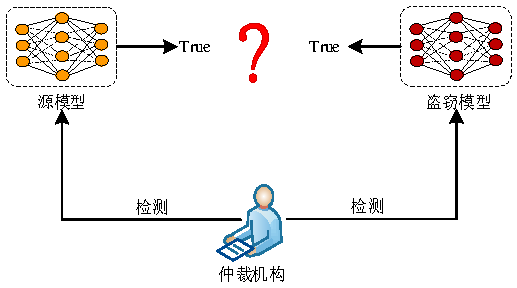
\includegraphics[width=0.6\linewidth]{检测歧义示意图.pdf}
	\caption{检测歧义示意图}
	\label{检测歧义示意图}
	%	\vspace{-3mm}  %调整图片标题与下文距离,与\setlength{\belowcaptionskip}{-3mm}等效。
\end {figure}

盗窃者对源模型嵌入新的水印或提取其他的指纹使原本的保护措施无效,歧义攻击对现有的深度神经网络模型的知识产权保护方法构成了严重威胁,在传统的数字水印领域中有研究表明,除非水印方案是不可逆的\cite{fan2019rethinking},否则鲁棒性的水印也不一定能验证所有权。

本文认为通过验证可疑模型是否具有源模型特定的水印或指纹来讨论盗窃行为是不充分的,特别是出现歧义攻击时,容易产生所有权混淆。因此本文提出推断模型所有权而不是验证,这是一种解决DNN模型所有权问题的新思路,与传统的通过模型水印和指纹验证所有权有所不同。这种方法是受数据集推断\cite{maini2021dataset}提出的数据驱动决策所有权的启发,利用某类数据在源模型上的最优性推断模型所有权,在下一小节中将具体讨论。


\section{模型所有权推断}\label{3.2}

数据集推断做了一个假设:源模型的知识来自于训练数据集。无论盗窃模型是直接攻击源模型还是其副产品,盗窃模型的知识仍然是源模型中包含的知识。如果原始训练数据集是私有的,那么模型所有者在进行数据集推断时,相比盗窃者拥有强大的优势,因为源模型在原始训练数据中的性能要远远优于其他数据集。因此,模型所有者通过评估多个数据点到分类边界的距离和统计测试相结合,可以得到模型的所有权归属。这种方式与模型水印和指纹验证所有权的方式有着本质的区别,该方式并不是去验证特定的水印或指纹,而是比较某类数据在模型上的最优性。

如图\ref{数据集推断原理图}所示,因为DNN模型是从数据集训练而来,所以模型中总会包含来自数据集中的知识。盗窃模型是从源模型派生,尽管包含的知识和源模型不可能完全相同,但总是有一部分是来自原始数据集,这是利用数据集做模型所有权推断的理论基础。

\begin{figure}[htbp]%%图,[htbp]是浮动格式
	\centering
	\setlength{\abovecaptionskip}{3mm} %图片标题与图片距离
	%	\vspace{-2mm}
	\setlength{\belowcaptionskip}{-3mm} %调整图片标题与下文距离
	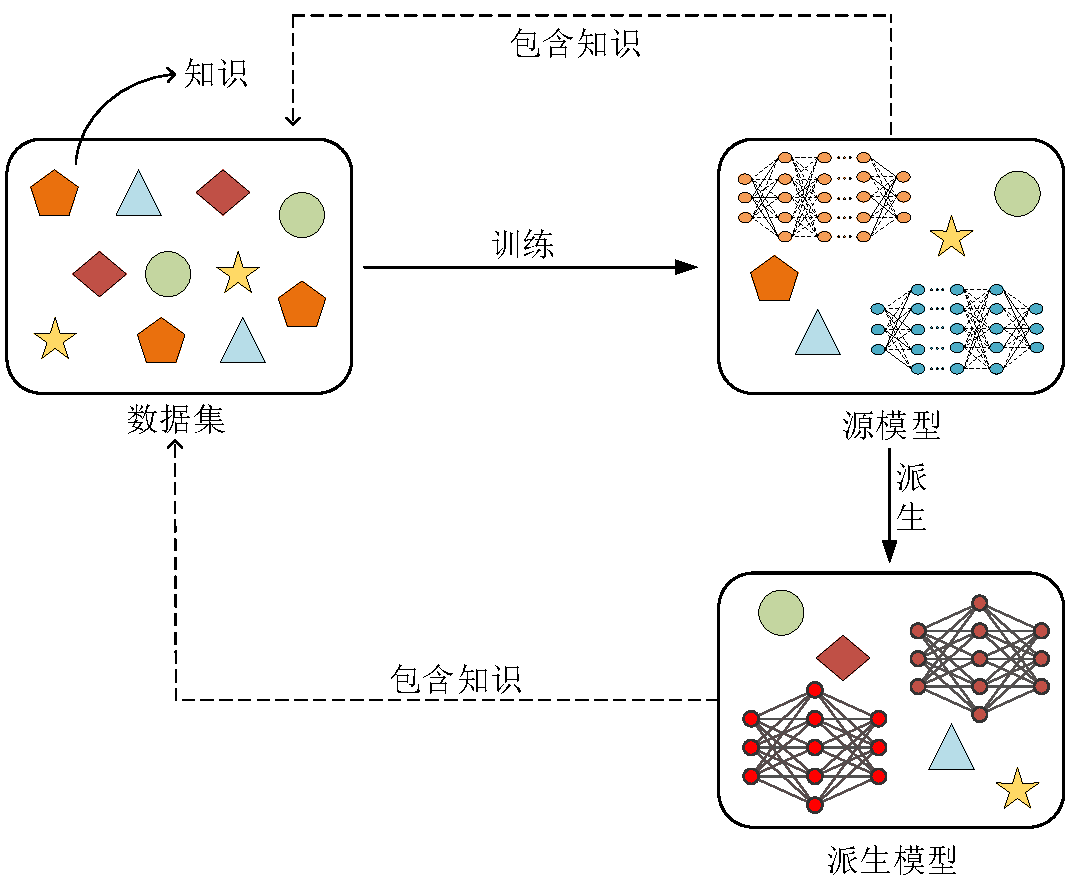
\includegraphics[width=0.8\linewidth]{数据集推断原理图.pdf}
	\caption{数据集推断原理图}
	\label{数据集推断原理图}
	%	\vspace{-3mm}  %调整图片标题与下文距离,与\setlength{\belowcaptionskip}{-3mm}等效。
\end {figure}	

模型窃取过程中,源模型中的知识会传播到盗窃模型,使得所有盗窃模型总是包含一部分源模型训练数据集中的直接或间接信息。利用数据集做模型所有权推断和传统的验证模型所有权不同,通过私有数据集推断得到的是一个所有权决策,其中决策的最大者被认为拥有所有权。传统的模型所有权验证是从模型中提取水印或指纹进行匹配从而验证,这种方式容易受到歧义攻击,进而导致的验证冲突。从决策过程可以发现数据集推断得到的是一个“最”的概念,模型的所有权归属于决策指标的最大者,而不是进行类似模型水印和指纹的特定响应匹配,因此可以有效避免歧义攻击。

本文的工作是受到数据集推断验证模型所有权的启发,使用数据驱动推断模型所有权代替验证模型所有权。所有权推断可以在有效证明所有权归属的同时,解决所有权验证冲突的问题。除此之外,数据驱动的推断所有权意味着该方法只和DNN模型的输入输出相关,那么数据驱动推断模型所有权的方法既可以在白盒环境也可以在黑盒环境下工作。

利用数据来推断模型所有权为保护模型知识产权提供了一个新的方向,但是目前数据集推断的方式仍然具有以下\textbf{局限性}:

1)使用数据集推断的前提是原始训练数据不能被盗窃者获得,所以公开的数据集不能被用于训练源模型。然而,在大多数真实场景下,只有很少一部分工作会构造私有数据集用于训练模型,甚至这部分工作只应用于特定的领域中,这也意味着模型被盗窃的风险较小。因此,依赖于私有数据集的数据集推理方法在实际应用中使用范围很小,不能被大幅度推广使用。

2)数据集推断方法的核心思想是源模型的功能在训练数据上的效果优于其他数据,但是存在模型的功能可能相似,而结构和训练数据都不同的情况,因此该方法的结果可能会导致错误,将不相关模型判定为盗窃模型。Li等人\cite{lao2022deepauth}验证了这个局限性,表明在此种情况下该方法产生的结果值得怀疑。

因此,亟需一种模型知识产权保护方法,在能成功判断模型所有权归属的同时,解决歧义攻击问题,并且适用于公开数据集。本文提出的方法将基于近边界数据推断DNN分类模型所有权。


\section{初始近边界数据的生成}\label{3.3}

上一节提出使用数据驱动来推断模型所有权,为了使训练数据公开,本文需要寻找一种新的数据来代替训练数据进行推断。本节将介绍这种特殊的数据——近边界数据,并且研究生成近边界数据的算法。

\subsection{近边界数据的可继承性}

DNN分类器的主要目标是对输入数据样本进行分类,一个DNN分类器的特征通常由其决策模式和分类边界决定。然而,分类器的分类边界是一个抽象的概念,无法被具体表示,因此研究者一般通过某正常数据样本和对应生成的对抗性样本组成样本对用于反映分类边界。因为分类边界位于两者之间,所以一定规模的对抗样本对可以用于描述分类边界。由于无法以数学的方式直接定义分类边界,本文使用分类器的决策结果来反映分类边界。

在以往的研究中\cite{cao2021ipguard},可以使用分类边界作为模型指纹用于验证模型所有权。本文不使用分类边界作为模型指纹,而是基于分类边界构造一类特殊的数据用于推断模型所有权。本文称这类特殊的数据为近边界数据,下面给出本文近边界数据的定义:

\begin{Definition}[近边界数据]
	\label{def:1}
	给定数据样本$x$,阈值$\theta$,如果数据样本$x$满足$\vert g_i(x) - g_j(x) \vert \leq \theta$,其中$i \neq j $并且$min(g_i(x), g_j(x)) \geq \mathop{max} \limits_{k \neq i, j}g_k(x)$,$g_k(x)$代表数据样本$x$被决策为类别$k$的概率,则数据样本$x$被称为近边界数据。
\end{Definition}

近边界数据是指那些非常接近分类边界的数据样本,与位于分类边界上的数据样本类似,这些样本对模型的决策边界有重要的影响,因为它们能够揭示模型在分类边界附近的行为。由于近边界数据不要求样本完全位于分类边界上,因此即使模型受到修改,分类边界发生偏移,仍然可以衡量数据近边界性。所以相对于直接使用分类边界来作为模型指纹,近边界数据在面对模型窃取攻击时,有着更强的鲁棒性。

如图\ref{近边界数据示意图}所示,近边界数据位于DNN分类器的分类边界附近,其他数据的分布则离分类边界较远。判定是否为近边界数据由定义\ref{def:1}中的阈值$\theta$决定,当$\theta$较小时,近边界数据样本表现为更加靠近模型分类边界。

\begin{figure}[htbp]%%图,[htbp]是浮动格式
	\centering
	\setlength{\abovecaptionskip}{5mm} %图片标题与图片距离
	%	\vspace{-2mm}
	\setlength{\belowcaptionskip}{-3mm} %调整图片标题与下文距离
	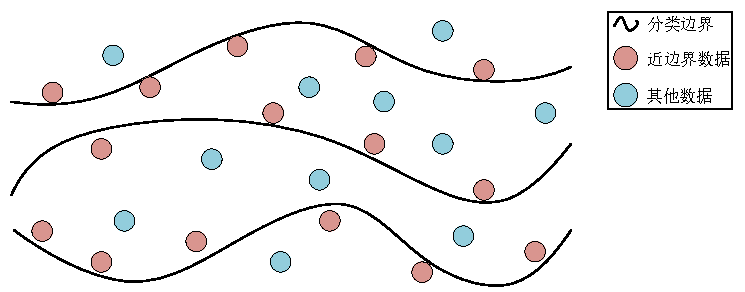
\includegraphics[width=0.9\linewidth]{近边界数据示意图.pdf}
	\caption{近边界数据示意图}
	\label{近边界数据示意图}
	%	\vspace{-3mm}  %调整图片标题与下文距离,与\setlength{\belowcaptionskip}{-3mm}等效。
	\end {figure}
	
在\ref{5}\ref{5.4}中,本文通过大量的实验验证了近边界数据在大多数的模型窃取技术中其近边界特征被保留,表明近边界数据的近边界性可以很好的继承到源模型派生出的模型上。因此,近边界数据可以作为推断所有权的依据被使用。尽管近边界数据在模型的知识产权保护中表现出显著的效果,但是在实践中,获得一定规模的近边界数据样本仍然是一个具有挑战性的任务。这是因为自然的近边界数据在样本空间中的占比非常低,甚至可以被忽略不计。通常来说,寻找位于分类边界上的数据点采用重复随机采样数据点的方法,然而,简单的重复采样可能需要大量的时间消耗,甚至无法找到这样的数据点。因此,如何得到一定规模的近边界数据样本仍然是一个难题,生成近边界数据的过程将在下一节中详细介绍。

\subsection{初始近边界数据的生成}

根据最近的一些研究\cite{cao2021ipguard},对抗性样本通常被用于确定分类器的分类边界。具体而言,对抗性样本有两个分类:原始分类和目标分类。其中,原始分类是指该样本不经过特殊处理的原始分类结果,目标分类是对原始样本添加微小噪声后的分类结果。对抗性样本是通过向原始数据添加小量扰动或干扰来生成的,这些扰动通常很难被人眼察觉,但却足以改变DNN模型的分类结果。

如图\ref{原始样本与对抗性样本对比}所示,对抗性样本对分类边界的跨越体现在,在视觉上,对抗性样本和原始样本几乎没有差别,但是分类结果却完全不同,在有目标攻击的情况下,甚至可以人为的指定目标分类。

\begin{figure}[htb]%%图,[htbp]是浮动格式
\setlength{\abovecaptionskip}{3mm} %图片标题与图片距离
\vspace{-2mm}
\setlength{\belowcaptionskip}{-3mm} %调整图片标题与下文距离
\subfigure[原始样本]{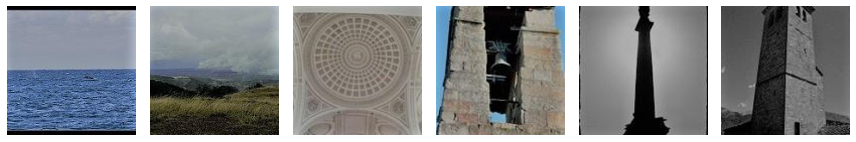
\includegraphics[width=1\linewidth]{原始样本.pdf}}
\subfigure[对抗性样本]{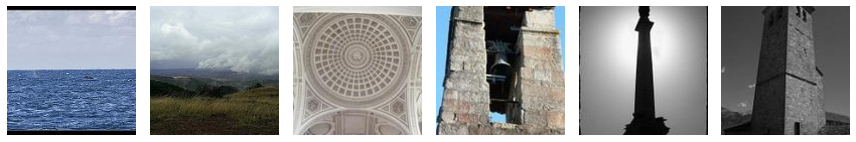
\includegraphics[width=1\linewidth]{对抗性样本.pdf}}
\caption{原始样本与对抗性样本的对比}
\label{原始样本与对抗性样本对比}
\end {figure}

对抗性样本会对模型分类边界进行跨越,本文认为该特征可以帮助获得较多的近边界数据。具体来说,本文将生成大量的对抗性样本,并从中挑选合适的近边界数据。因此,本文测试了几种常见的生成对抗性样本的方法,以帮助更好的构建近边界数据。因为本文需要数据样本尽可能靠近分类边界,因此在测试过程中,不同方法的优劣取决于生成对抗性样本到分类边界距离的远近,距离近者更优。

为了更好的衡量数据样本到分类边界的距离,在定义\ref{def:1}的基础上,下面给出量化的分类边界距离定义:

\begin{Definition}[分类边界距离]
	\label{def:2}
	给定一个数据样本$x$,它到分类边界的距离$distance = \vert g_i(x) - g_j(x) \vert$,其中$i \neq j $并且$min(g_i(x), g_j(x)) \geq \mathop{max} \limits_{k \neq i, j}g_k(x)$,$g_k(x)$代表数据样本$x$被决策为类别$k$的概率。
\end{Definition}

根据定义\ref{def:2},以分类边界距离为衡量标准,下面分别对几种常见的生成对抗性样本的方法进行介绍与测试。


\noindent\textbf{Fast \ Gradient \ Sign \ Method(FGSM):}FGSM \cite{goodfellow2014explaining}是最经典的生成对抗性样本的方法之一,它是一种基于梯度构建对抗性样本的方法,属于无目标的攻击方式。只需要对原始样本添加一次微小的扰动$\eta$,如式\ref{eq:3.1},\ref{eq:3.2}所示,即可生成样本$x$的对抗性样本$\tilde{x}$,十分高效。

\begin{equation}
	\setlength\abovedisplayshortskip{-5mm}
	%	 	\setlength\belowdisplayshortskip{4mm}
	\label{eq:3.1}
	\eta = \epsilon \cdot sign(\bigtriangledown_xJ(\theta,x,y^*))
\end{equation}
\begin{equation}
	\label{eq:3.2}
	\tilde{x} = clip(x + \eta)
\end{equation}

其中$sign$是符号函数,$x$表示原始样本,$y^*$表示$x$的真实类别,$\theta$表示模型权重参数,$J$表示分类器损失函数,$\bigtriangledown_x$表示对原始样本$x$求偏导,$clip$函数是将样本投射回可行数据域,比如图像样本的像素点范围应该在$[0,1]$以内,$\epsilon$用来控制变化幅度大小。

FGSM 生成对抗性样本的速度非常快,但其结果非常依赖$\epsilon$的选择,因此探索不同的$\epsilon$是使用该方法的重点。

\noindent\textbf{Iterative \ Gradient \ Sign \ Method(IGSM):}IGSM\cite{kurakin2018adversarial}是FGSM的进阶版本,如式\ref{eq:3.3},\ref{eq:3.4}所示,与FGSM只进行一次扰动叠加不同,IGSM采用迭代的形式构造对抗性样本,每次叠加一个小扰动。这个过程持续到成功生成对抗性样本或者达到迭代次数上限为止。

\begin{equation}
	\setlength\abovedisplayshortskip{-5mm}
	\label{eq:3.3}
	\eta = \alpha \cdot sign(\bigtriangledown_xJ(\theta,x,y^*))
\end{equation}
\begin{equation}
	\label{eq:3.4}
	\tilde{x}_t = clip(\tilde{x}_{t - 1}  + clip_{\epsilon}(\eta))
\end{equation}

\noindent $\alpha$是步长大小,$\tilde{x}_t$表示第$t$次迭代后的结果,$clip_{\epsilon}$是限定每次叠加的范围不超过$\epsilon$,其余参数含义与FGSM保持一致。

除此之外,本文还测试了FGSM的另一个进阶版本RFSGM\cite{tramer2017ensemble},RFSGM增加了扰动的多样性,可以更精细地生成对抗性样本。在实际结果中,发现尽管FGSM生成对抗性样本速度非常快,但是对抗性样本距离分类边界的距离比较远。IGSM 和RFGSM 效果要比FGSM 好,但仍然没有达到本文的预期,生成的对抗性样本距离分类边界距离太远。在大量的测试中,本文发现CW能够生成大量位于分类边界附近的样本,具体的测试结果在\ref{5}\ref{5.2}中。

\noindent\textbf{Carlini \ and \ Wagner's \ methods(CW):}CW\cite{carlini2017towards}方法是一种有目标的攻击方式,与其他生成对抗性样本的方法类似,该方法是添加噪声到数据样本中,但其具有三种变体:CW-$L_0$,CW-$L_2$和CW-$L_{\infty}$。不同的变体使用不同的方法来衡量噪声的大小,其中CW-$L_2$在实验中生成对抗性样本的效果和生成效率相比其余两种变体较好,因此本文使用该方法作为生成对抗性样本的基础。具体而言,CW-$L_2$对于给定的初始样本,采用二分查找的方式来增大或减小式\ref{eq:3.7}中$c$,并且使用类似训练神经网络模型的方式来调整生成对抗性样本的其他参数。CW-$L_2$的损失函数和约束如式\ref{eq:3.5},\ref{eq:3.6},\ref{eq:3.7},\ref{eq:3.8}所示:
\begin{equation}
	%	\setlength\abovedisplayshortskip{-8mm}
	\label{eq:3.5}
	Loss = Loss1 + Loss2 
\end{equation}
\begin{equation}
	%	\setlength\abovedisplayshortskip{-8mm}
	\label{eq:3.6}
	Loss1 = D(x, x + \delta)
\end{equation}
\begin{equation}
	%	\setlength\abovedisplayshortskip{-5mm}
	\label{eq:3.7}
	Loss2 = c \cdot f(x + \delta,target)
\end{equation}
\begin{equation}
	%	\setlength\abovedisplayshortskip{-5mm}
	%	\setlength\belowdisplayshortskip{-3mm}
	\label{eq:3.8}
	x + \delta \in [0,1]^m
\end{equation}

其中$target$是生成对抗性样本的目标标签,$c$是惩罚因子,用于权衡$Loss2$的影响大小,算法通过二分查找来寻找合适的$c$。$Loss1$约束对抗性样本$x + \delta$和原始样本$x$尽可能相似,$Loss2$约束对抗性样本$x + \delta$的决策结果为目标标签,式\ref{eq:3.8}约束对抗性样本在正常的图像范围内。

\begin{algorithm}[H] 
	\setstretch{1.2}
	\small
	\caption{\small 改进的二分查找CW-$L_2$算法}
	\label{alg:1}
	%	\small
	\begin{algorithmic}[1]
		\Require 样本$x$;模型$M$;阈值$\theta$;二分次数$n$;迭代次数$iteration$;原始标签$r$;目标标签$t$
		\Ensure 近边界对抗性样本$x'$
		\State 参数初始化:$c\gets1$,$distance \gets 1$
		\For {$i=1,2,...,n$}
		\State $isSuccessAttack \gets$ false
		\State $w \gets$ arctanh($x$)
		\State $w\_pert \gets$ zero\_like($w$)
		\For{$j=1,2,...,iteration$}
		\State $new\_img \gets$ tanh($w + w\_pert$)
		\State $new\_distance \gets\vert g_r(new\_img) - g_t(new\_img) \vert$
		\If{$new\_distance < distance$}
		\State $distance \gets new\_distance$
		\State $x' \gets new\_img$
		\State $isSuccessAttack \gets$ true
		\EndIf
		\State 使用Adam优化器更新$w\_pert$
		\EndFor
		\If{$isSuccessAttack$ == true}
		\State 减小$c$
		\Else \State 增大$c$
		\EndIf 
		\If{$distance \leq \theta$} 
		\State break
		\EndIf
		\EndFor
		\State \textbf{return} $x'$
	\end{algorithmic}
	
\end{algorithm}

根据定义\ref{def:2},数据样本$x$距离分类边界的距离是$distance = \vert g_i(x) - g_j(x) \vert$。本节的目标是生成的对抗性样本距离分类边界的距离尽可能近。本文在算法迭代过程中引入这一目标,以此改进算法迭代的过程,在使得生成对抗性样本更加靠近分类边界的同时,提高算法效率。具体而言,在迭代过程中,仅在$distance$变小时,更新距离参数和新生成的对抗性样本,并在$distance$小于等于预定的阈值$\theta$时,提前终止算法的迭代,具体的过程如算法\ref{alg:1}所示。





通过算法\ref{alg:1},本文已经可以生成大量位于分类边界附近的近边界数据。但是在这一阶段,本文只是在源模型的样本空间中挑选一部分数据作为初始样本添加微小噪声或扰动,针对性地生成了目标分类的对抗性样本。

在此阶段,源模型的训练和原始训练数据集均不受任何影响,防御者只需要针对性的生成对抗性样本即可。然而,近边界数据作为推断所有权的重要证据,直接生成对抗性样本也极易受到盗窃者的伪造。因此,本文需要将生成的近边界数据私有化,防止被盗窃者轻易伪造,具体操作将在下一节中给出。

\section{本章小结}

本章首先分析了现有的通过模型水印和模型指纹来做所有权验证的局限性,然后提出数据驱动的推断所有权的方法。鉴于近边界数据在源模型和其派生模型上的可继承性,本文使用近边界数据来代替训练数据进行所有权推断。由于自然的近边界样本很少,本文对比了主流的对抗性样本生成算法,根据生成样本到分类边界的距离。选择CW-$L_2$作为基础算法。并在此基础上改进,生成本文的初始近边界数据。
% !TeX root = ../main.tex
% -*- coding: utf-8 -*-

\chapter{基于近边界数据的模型所有权推断方法}\label{4}

尽管训练数据可以被公开,但用于推断模型所有权的数据需要私有化,否则攻击者就可以轻易地伪造近边界数据,无法成功推断模型所有权。因此本章通过生成对抗网络来对近边界数据进行特征学习,进而通过生成器生成新的、私有化的近边界数据。在此基础之上,使用私有化近边界数据微调源模型,使私有化近边界数据更靠近模型分类边界,数据越靠近分类边界,越有利于成功推断模型所有权。

结合上一章生成的初始近边界数据,本文方法的整体流程如图\ref{方法流程图}所示,主要包括三个阶段:(1)从公开数据集中生成近边界数据,(2)训练生成对抗模型生成新的、私有化的近边界数据,(3)使用私有化近边界数据微调源模型分类边界。

\begin{figure}[htbp]%%图,[htbp]是浮动格式
	\centering
	\setlength{\abovecaptionskip}{5mm} %图片标题与图片距离
%	\vspace{1mm}
%	\setlength{\belowcaptionskip}{-3mm} %调整图片标题与下文距离
	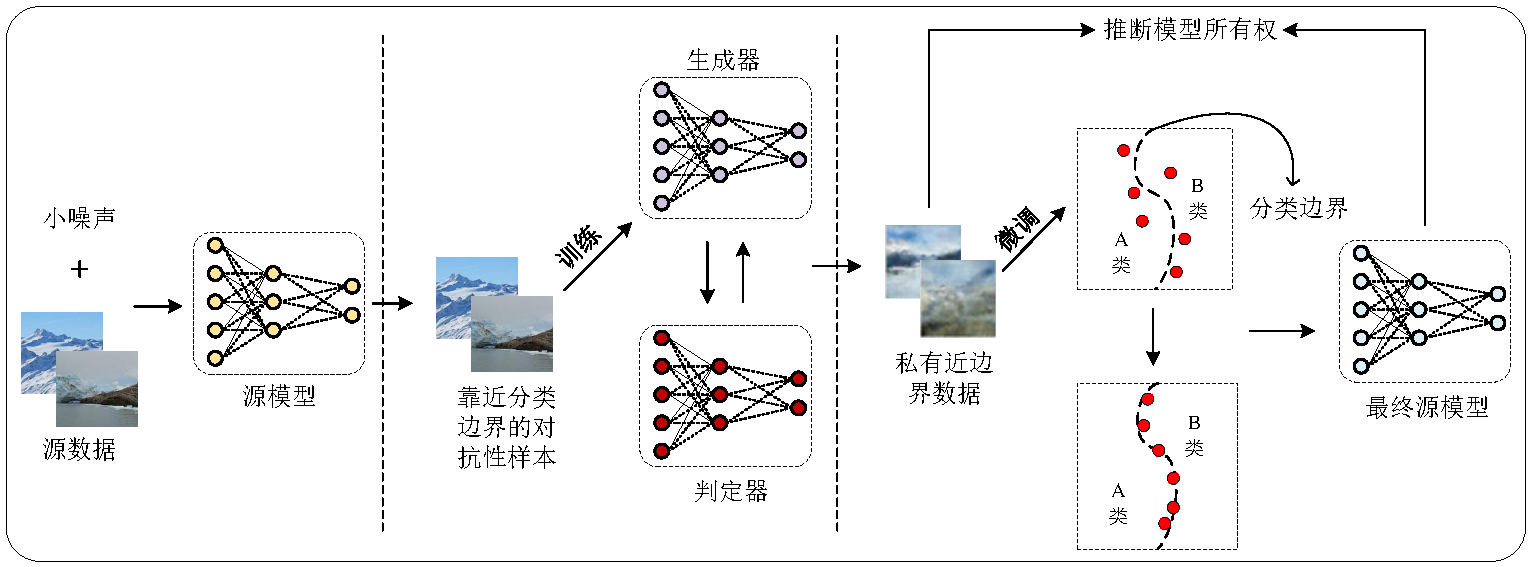
\includegraphics[width=1\linewidth]{方法流程图.pdf}
	\caption{方法流程图}
	\label{方法流程图}
	%	\vspace{-3mm}  %调整图片标题与下文距离,与\setlength{\belowcaptionskip}{-3mm}等效。
	\end {figure}



\section{近边界数据私有化}\label{4.1}

因为现在大多数模型训练使用的数据都来源于公开的数据集,所以通过生成对抗性样本的方法构建近边界数据这一步骤也十分容易复现。因此,本文需要从公开的训练数据中构建自己的私有化近边界数据,以防止模型所有者的近边界数据被轻易模仿。这是必要的步骤,因为近边界数据是后续推断模型所有权的核心依据。

本文希望可以通过训练一种模型学习上一节中生成的近边界对抗性样本的特征,并以此生成新的私有化近边界数据。这种新的数据从视觉上不一定和原始数据类似,但其原始的特征以及添加的噪声需要被学习,并根据提取到的特征生成的新样本对于源模型同样是近边界数据。

由\ref{2}\ref{2.3}可知,生成对抗网络在图像生成和特征提取方面有着显著的效果。本文考虑设计基于生成对抗网络的特征提取器,对初始近边界数据进行特征提取后,使用用生成器生成新的、私有化的近边界数据。

与生成初始近边界数据指标一致,本文需要寻找一种GAN,其生成的近边界数据到分类边界距离尽可能小。本文测试了几种常见的图像生成GAN,包括边界寻求生成对抗性网络(Boundary-Seeking Generative Adversarial Networks, BGAN)\cite{devon2017boundary},边界平衡生成对抗网络(Boundary Equilibrium Generative Adversarial Networks, BEGAN)\cite{berthelot2017began}和基于深度卷积生成对抗网络(Deep Convolutional Generative Adversarial Network, DCGAN)\cite{radford2015unsupervised}。大部分情况下,DCGAN的效果最好,具体的测试结果在\ref{5}\ref{5.3}中。因此,本文设计了一种基于DCGAN的特征提取器,提取近边界数据的特征之后,使用生成器生成私有化的近边界数据。
%注意生成器以,$CW$-$L_2$生成的对抗性示例作为输入,并输出私有化后的近边界数据。

\begin{figure}[htbp]%%图,[htbp]是浮动格式
	\centering
	\setlength{\abovecaptionskip}{5mm} %图片标题与图片距离
	%	\vspace{-2mm}
	\setlength{\belowcaptionskip}{-3mm} %调整图片标题与下文距离
	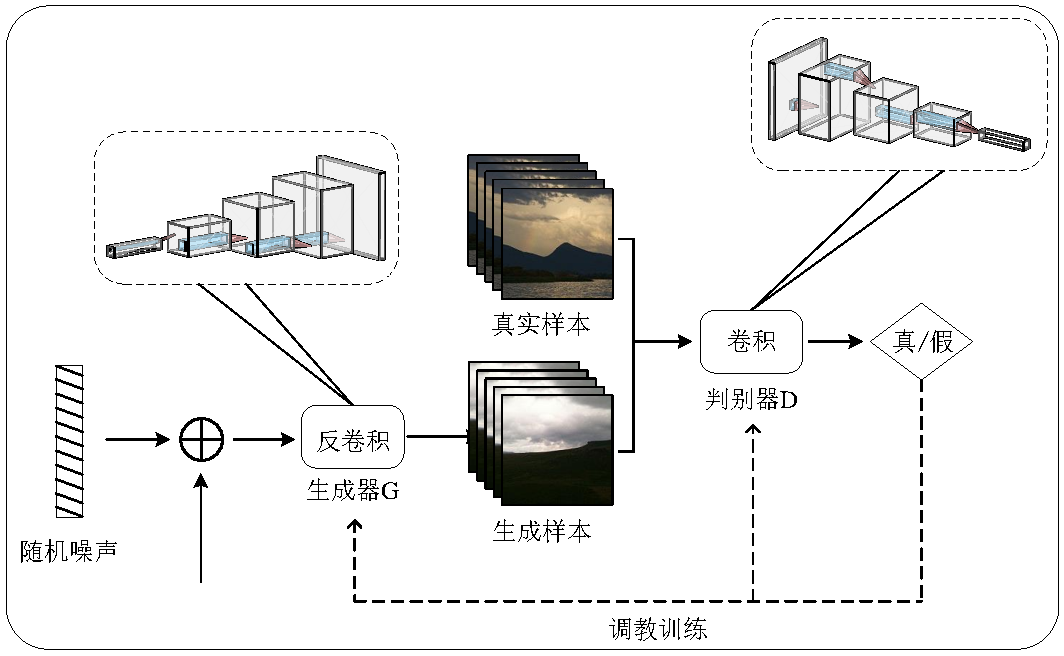
\includegraphics[width=1\linewidth]{DCGAN网络结构图.pdf}
	\caption{DCGAN网络结构图}
	\label{DCGAN网络结构图}
	%	\vspace{-3mm}  %调整图片标题与下文距离,与\setlength{\belowcaptionskip}{-3mm}等效。
	\end {figure}
	
如图\ref{DCGAN网络结构图}所示,DCGAN的大体结构与训练方式和普通GAN类似,主要变化是DCGAN将原始的GAN与CNN结合到一起,生成器$G$和判定器$D$都用CNN架构替换了原始GAN的全连接网络。得益于CNN对图像的强大处理能力,DCGAN极大提升了网络训练稳定性和生成样本的质量。具体而言,DCGAN主要是从网络架构上改进了原始的GAN,主要改进如下:

1)DCGAN的生成器和判别器均舍弃掉CNN的池化层,生成器使用反卷积层来还原图片,判别器保留CNN的整体架构,使用卷积层来提取图片特征。

2)在生成器和判别器中都使用Batch Normalization层,提升训练DCGAN模型稳定性的同时加速了训练。

3)生成器除最后一层使用Tanh激活函数外,其余层使用ReLU,判别器所有层均使用LeakyReLU,使模型可以更快的学习。

4)使用Adam优化器并调整了超参数,将学习率设置为0.0002,可以更好的学习到数据样本的特征。

本文需要DCGAN能够学习到尽可能多的近边界数据特征,以便更好的生成近边界数据。训练过程中,尝试修改DCGAN判定器的目标函数,在保留梯度的情况下,将其与源模型的结果相连,即使用源模型和判别器共同判定是生成数据还是原始数据。这种方式得到的训练结果在同样的生成规模下略微优于原始DCGAN生成的数据。然而,考虑到两者的效率,实际情况下生成的结果并无较大区别,所以本文采用原始的训练方式。训练DCGAN的具体流程如算法\ref{alg:2}所示。

\begin{algorithm}[!h] 
	\setstretch{1.2}
	\caption{\small 训练DCGAN模型}
	\label{alg:2}
	\small
	\begin{algorithmic}[1]
		\Require 近边界数据$\tilde{D}$;批处理大小$batchsize$;训练轮次$epoch$;损失函数$Loss$
		\Ensure 训练好的DCGAN模型
		\State 参数初始化:$learning \ rate \gets 0.0002$,$real\_label \gets 1$,$fake\_label \gets 0$
		\For{$i=1,2,...,epoch$}
		\State 随机噪声$z \gets 100$ 
		\State $x' \gets G(z)$
		\State $Loss1 \gets Loss(D(x), real\_label)$  \Comment $x$是近边界数据样本
		\State $Loss2 \gets Loss(D(x'), fake\_label)$
		\State $Loss_D \gets Loss1 + Loss2$
		\State $Loss_G \gets Loss(D(x'), real\_label)$ \Comment 生成器希望$D(x') $接近$real\_label$
		\State 使用Adam更新生成器$G$,判别器$D$的网络参数
		\EndFor
	\end{algorithmic}
	
\end{algorithm}

通过算法\ref{alg:2},完成训练DCGAN模型后,该模型可以被用作近边界数据特征提取器。通过生成器生成的图像,可以生成与初始近边界数据分布一致的私有近边界数据,这些数据仍然具备近边界性,并且可疑对手无法轻易获得。

在DCGAN的训练过程中,生成器和判定器相互博弈,以不断优化生成器生成图像的特征分布,使其逐渐接近原始近边界样本。训练收敛时,生成器已经学习到近边界数据的特征,因此可以生成新的私有近边界数据。

\section{源模型分类边界的微调}\label{4.2}

DCGAN对图像数据有着很强的特征提取能力,生成器能够很好的学习近边界数据特征,使用生成器构建的私有近边界数据仍然位于目标分类边界附近。但是相比于原始近边界数据,由于随机因素,生成的数据样本近边界性可能会弱于原始近边界数据,本文仍然希望近边界数据能最大程度上靠近目标分类边界。因为近边界数据与目标分类边界的距离越近,推断模型所有权成功的可能性就越大。此外,生成的私有近边界数据虽然只被模型所有者拥有,但对于一些功能易被泛化的模型,经过模型窃取攻击后,由于模型被修改,数据的近边界特性仍有可能被泛化。

因此,为了解决上述问题,本文提出使用近边界数据微调源模型的目标分类边界,使生成的私有近边界数据更加靠近DNN模型分类边界。如式\ref{eq:3.4}所示,$Loss_{FT}$是针对目标分类边界的损失函数。
\begin{equation}
	%	\setlength\abovedisplayshortskip{-3mm}
	\label{eq:3.9}
	Loss_{FT} = \frac{1}{n} \sum^{n}_{i = 1} (g_t(x_i') - g_s(x_i'))^2
\end{equation}

其中$n$是该目标分类边界的近边界数据的数量,$x_i'$是生成的近边界数据,$g_t(\cdot)$和$g_s(\cdot)$分别表示目标分类概率和源分类概率。

$Loss_{FT}$本质是希望近边界数据更靠近目标分类边界,但是为了尽可能减小对原始模型精度的影响,不能直接使用该损失函数对源模型进行微调。受DCGAN训练过程的启发,本文使用源模型的损失函数$Loss_{FM}$与$Loss_{FT}$两者交替训练微调源模型,并将学习率设置为0.0001,尽量减小源模型的变化幅度。本文希望在保持源模型精度的同时,使生成的数据样本更加靠近目标分类边界。与DCGAN的训练过程相似,微调源模型也是一个博弈的过程,微调的具体流程如算法\ref{alg:3}所示。

\begin{algorithm}[H] 
	\setstretch{1.2}
	\caption{\small 微调源模型}
	\label{alg:3}
	\small
	\begin{algorithmic}[1]
		\Require 原始数据集$D$;私有化近边界数据$D'$;批处理大小$batchsize$;训练轮次$epoch$;损失函数$Loss_{FT}$,$Loss_{FM}$;源模型$M$
		\Ensure 微调后的源模型$M'$
		\State 参数初始化:$learning \ rate \gets 0.0001$
		\For{$i=1,2,...,epoch$}                          
		\State $Loss1 \gets Loss_{FT}(g_t(x') , g_s(x'))$ \Comment $g_k(x')$:$x'$在第$k$类上的概率
		\State $Loss2 \gets Loss_{FM}(M(x), label)$ \Comment $label$指正常样本的原始标签
		\State 使用Adam更新源模型$M$的网络参数
		\EndFor
	\end{algorithmic}
	
\end{algorithm}

其中$x$指原始的数据样本,$x'$指DCGAN生成器生成的私有化近边界数据。

通过算法\ref{alg:3}微调目标分类边界使得私有近边界数据与源模型之间的联系更加紧密,这对后续能否成功推断模型所有权十分重要。在此算法中,本文只微调目标分类边界,且通过交替微调尽可能减少微调对源模型的影响。

\begin{table}[h]
	\centering
	%	\setlength{\arrayrulewidth}{0.5mm}
	\renewcommand\arraystretch{1.2}
	\caption{微调分类边界对模型的影响}
	\label{table:state}
	\small
	\begin{tabular*}{13cm}{@{\extracolsep{\fill}} l c c}
		
		
		
		\toprule[1pt]
		\textbf{数据集}        &    \textbf{微调前准确率}   &   \textbf{微调后准确率}            \\
		\hline
		CIFAR-10      &     0.886        &     0.873               \\
		
		Heritage      &     0.879        &     0.866               \\
		
		Intel\_image  &     0.854        &     0.846               \\
		\bottomrule[1pt]		
	\end{tabular*}
	
\end{table}

如表\ref{table:state}所示,正因为交替微调的设计和较小的学习率,源模型微调前后的精度差不超过3\%。因此,微调对于源模型的性能影响十分微小,甚至可以被忽略,但却有效提高了最后的所有权推断效果。更多微调目标分类边界对准确度的影响测试在\ref{5}\ref{5.4}中。

\section{推断可疑模型所有权}\label{4.3}

本文的方法适用于DNN分类模型的知识产权保护。一方面,该方法是利用近边界数据进行所有权推断,决策双方各自提供自己的近边界数据。将这些数据分别输入模型后,距离分类边界最近的数据提供者,获得模型的所有权,而不是进行类似模型水印和指纹的特定响应匹配,因此可以有效避免歧义攻击。另一方面,针对现有的数据集推断方法存在的问题,主要有以下两点改进:

1)本文在公开数据集上生成近边界数据代替私有训练数据,并且通过训练生成对抗网络生成新的、私有化的近边界数据,在解决数据集推断只能用于私有训练数据集问题的同时,也防止了本文的近边界数据被轻易复制和模仿,保持私有数据在推断模型所有权时的优势。

2)本文的方法利用近边界数据靠近决策边界的特性解决模型功能相似引起的误导。这是因为即使模型功能相似,但是决策边界不可能完全相同。如果近边界数据在可疑模型上并没有表现出近边界性,那么不会判定该模型是盗窃模型。\ref{5}\ref{5.4}中验证了这一点,本文提出的近边界数据,在无关模型上不会表现出近边界性。

\noindent\textbf{问题定义:}本文定义了一个DNN分类器$G$作为源模型,给定一个原始训练集$D$,假设该源模型是一个$n$-类的DNN分类器,分类器的输出层为softmax层或其他决策层,决策函数$g_j(x)$表示数据样本$x$被分到第$j$类的概率,其中$j$ = 1,2,..,$n$。$Z_1$,$Z_2$,..,$Z_n$表示模型分类器的全部决策函数输出,其结果可作为分类边界的依据被本文使用,因此

\begin{equation}
	g_j(x) = \frac{exp(Z_j(x))}{\sum_{i = 1}^n exp(Z_i(x))}
\end{equation}

\noindent 其中,数据样本$x$的标签$y$被推断拥有最大概率的类别,例如$y = arg \mathop{max} \limits_j g_j(x) = arg \mathop{max} \limits_j Z_j(x)$。

\subsection{设计目标}

根据现有的工作,本文提出的的方法在源模型训练后进行部署,且在黑盒环境下推断模型所有权。本文的方法不关注模型被盗窃的过程,而是聚焦在准确地推断DNN模型的所有权和识别不法分子的模型盗窃行为。现在大多数所有权验证技术都是基于黑盒环境。因为模型所有者和攻击者通常不会提供完整模型,而是以API的形式提供商业服务,因此黑盒模式的适用情况更加广泛。本文提出的方法仅利用模型提供的外部API,获取近边界数据的决策结果,从而推断模型所有权。

在通常的假设中,存在一个官方的仲裁机构,当对任一模型产生所有权怀疑时,受害者和可疑对手可以向机构提出申请并提供各自的私有化近边界数据,并通过本文的方法推断所有权。无论是在白盒的环境还是在黑盒的环境下,本文提出的方法均可以用来推断模型所有权。

本文提出的方法需要在面对各种盗窃模型时成功推断模型所有权,与此同时,需要保持DNN模型的性能并且不能对无关模型产生错误的所有权误导。因此本文提出方法的设计目标如下:

1)\textbf{精确性:}推断模型所有权的方法不应该影响模型的性能,模型的最大可接受测试精度下降不超过3\%。

2)\textbf{可继承性:}如果可疑模型与源模型相同或从源模型派生而来,则私有近边界数据在这些模型中均表现出近边界性。反之,近边界数据在无关模型中没有明显特征,防止产生所有权推断误导。

3)\textbf{有效性:}如果可疑模型与源模型相同或从源模型派生而来,则根据源模型构造的私有近边界数据比其他近边界数据更加靠近分类边界,这是本文方法成功推断模型所有权的依据。

4)\textbf{鲁棒性:}近边界数据应该对常见的模型修改(如模型微调、剪枝和有损压缩)具有鲁棒性,这是本文方法能广泛应用的关键。

5)\textbf{不可获得性:}敌手无法获得私有的近边界数据,否则私有近边界数据不在有更加靠近分类边界的优势,无法成功推断模型所有权。

6)\textbf{高效性:}通过近边界数据推断模型所有权应该能够高效地计算距离边界数据,并通过对比全部近边界数据的决策结果确定可疑模型是否是盗窃模型。

本文将在\ref{5}对该方法进行详细的实验评估,实验评估后,逐一验证分析是否达到这6个设计目标。

\subsection{方法概述}

本文提出了近边界数据,一种分布在分类边界附近的特殊样本。模型指纹使用对抗性样本抽象地反映模型分类边界,同一组对抗性样本的输入,其引起的决策模式的变化可以用于比较模型知识的相似性,但这种方法是脆弱的,一般的模型窃取攻击都会修改源模型,而对模型的任意修改操作都有可能破坏这种特性。因此,本文不直接比较决策模式的变化,它是不可信任的,而是比较对抗性样本与决策边界的距离。大多数对抗性样本都是位于决策边界附近的,也就是说,它们与决策边界的距离很近。对抗性样本的这种性质被本文所利用并构造近边界数据,经过测试,本文发现绝大多数的模型窃取方法都无法改变这种结果,即使样本分类被影响,其仍然位于分类边界附近。

近边界数据背后的意义是数据的近边界特性不会因为受到模型窃取攻击产生的模型修改而消失。受到这个特点的启发,将近边界数据作为水印验证所有权是传统的思路,虽然不会对模型的精度造成影响,但是这样的水印是脆弱的,很容易受到御歧义攻击,因此本文提出由近边界数据驱动的所有权推断方法。
%\begin{figure}[htb]%%图,[htbp]是浮动格式
%	\centering
%	\setlength{\abovecaptionskip}{5mm} %图片标题与图片距离
%	%	\vspace{-2mm}
%	\setlength{\belowcaptionskip}{-3mm} %调整图片标题与下文距离
%	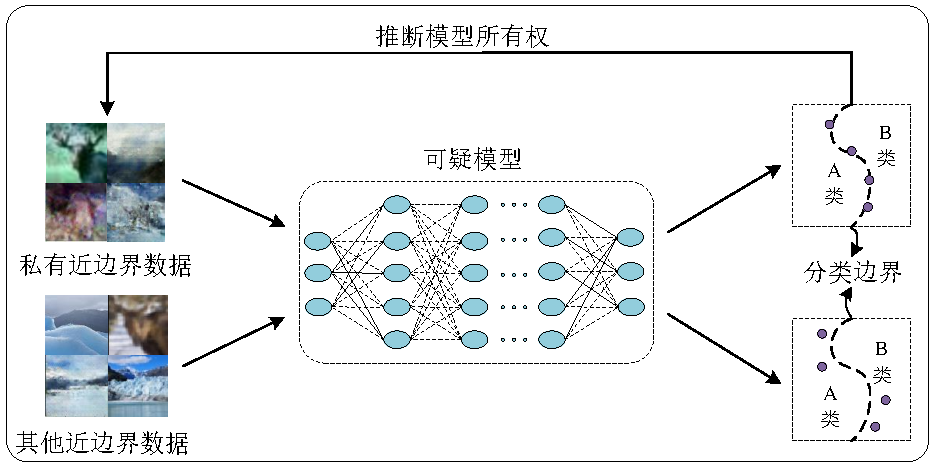
\includegraphics[width=1\linewidth]{方法原理图.pdf}
%	\caption{近边界数据推断所有权}
%	\label{方法原理图}
%	%	\vspace{-3mm}  %调整图片标题与下文距离,与\setlength{\belowcaptionskip}{-3mm}等效。
%	\end {figure}

\begin{figure}[htbp]%%图,[htbp]是浮动格式
	\centering
	\setlength{\abovecaptionskip}{5mm} %图片标题与图片距离
	%	\vspace{-2mm}
%	\setlength{\belowcaptionskip}{-3mm} %调整图片标题与下文距离
	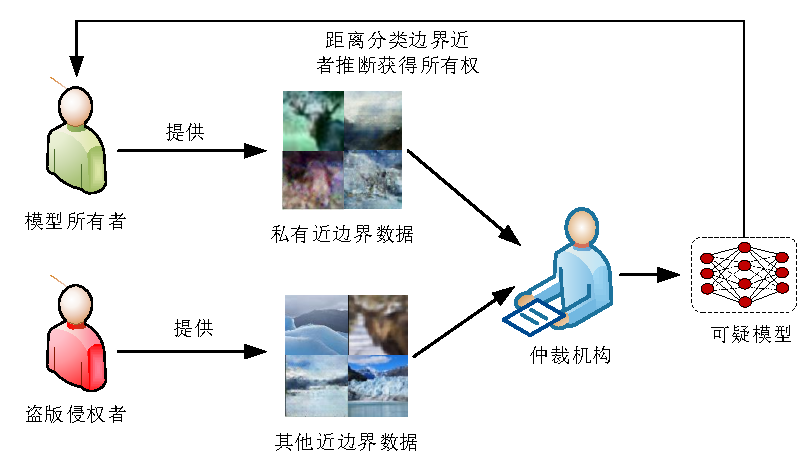
\includegraphics[width=0.8\linewidth]{推断示意图.pdf}
	\caption{推断示意图}
	\label{推断示意图}
	%	\vspace{-3mm}  %调整图片标题与下文距离,与\setlength{\belowcaptionskip}{-3mm}等效。
	\end {figure}

如图\ref{推断示意图}所示,本文提出方法的主要思想是构造私有的近边界数据,以数据驱动推断模型的所有权。当模型所有者怀疑可疑模型是盗窃自己的模型时,向官方机构发起仲裁。模型所有者和可疑对手分别提供各自的私有近边界数据,仲裁机构分别计算双方数据的输出结果,统计测试样本数据点到分类边界的距离,距离近的判定获得模型所有权。


\subsection{假设检验}\label{3.3.3}

根据\ref{3}的讨论结果,本文认为过去的验证模型所有权的思路具有较大的局限性,大多数研究无法抵御歧义攻击。因此,本文提出了推断模型所有权的方法,这是一种“最”的思路。与过去工作中利用模型水印和指纹验证模型所有权相比,本文方法使用数据在对应模型上结果作为所有权推断依据,结果的可比性和唯一性可以有效避免歧义攻击。

上一小节中提到,模型所有者向仲裁机构提出仲裁并提供近边界数据,盗窃者同样需要提供相应的近边界数据,仲裁机构分别计算各自数据到目标分类边界距离,最靠近目标分类边界的近边界数据所有者将获得模型所有权。由于近边界数据通常是一组数据,所以应该根据统计的结果来看。在实验中,本文计算了不同规模的近边界数据组在源模型、盗窃模型以及不相关模型上到分类边界的距离,并设计了一种基于假设检验的方法来表现推断的置信度。

\noindent\textbf{假设检验:}本文假设事件$C$是模型所有者提供的私有近边界数据在可疑模型上的计算结果,事件$C_S$ 表示盗窃者提供的近边界数据在可疑模型上的计算结果,或模型所有者提供的私有近边界数据在无关模型上的计算结果。本文计算假设$H_0:\mu \geq \mu_S(H_1:\mu < \mu_S)$的$p$值,以及差异大小$\Delta \mu = \mu_S - \mu$,$\Delta\mu$越大,推断可信度越高。如果$p$值低于预定义的置信度评分$\alpha$,则拒绝$H_0$,并称正在测试的模型是被盗模型。本文重复30次统计性实验以提高可信度,假设检验的具体过程如算法\ref{alg:4}所示。

\begin{algorithm}[H] 
	\setstretch{1.2}
	\caption{\small 假设检验}
	\label{alg:4}
	\small
	\begin{algorithmic}[1]
		\Require 模型所有者私有近边界数据样本$X$;可疑对手近边界数据样本$X_S$;可疑模型$\tilde{M}$;假设检验对照表$T$;显著性水平$\alpha$
		\Ensure 可疑模型是否为盗窃模型
		\State 原假设:$H_0:\mu \geq \mu_S$
		\State 备择假设:$H_1:\mu < \mu_S$
		\State 计算模型所有者私有近边界数据样本均值$\overline{X}$                     
		\State 计算可疑对手近边界数据样本均值$\overline{X}_S$ 
		\State 计算统计量$t$
		\State 查对照表$T$获得临界值$\lambda$
		\If{$t > \lambda$}
		\State $p < \alpha$,拒绝$H_0$,接受$H_1$,可疑模型是被盗模型
		\Else \State $p > \alpha$,不拒绝$H_0$
		\EndIf
	\end{algorithmic}
\end{algorithm}

结合生成使用CW-$L_2$生成初始近边界数据和使用DCGAN私有化近边界数据的过程,加上假设检验比对结果的差异性,本文提出方法的整体执行流程如图\ref{方法整体流程图}所示。



\section{本章小结}

近边界数据是本文方法推断所有权的依据,不能轻易被盗窃者复制伪造。本章使用初始近边界数据训练DCGAN,使之学习到近边界数据的特征,然后使用生成器生成新的、私有化的近边界数据,使所有者保持私有数据的优势。接着设计了新的损失函数并微调源模型,使近边界数据更加靠近目标分类边界,增强本文方法面对各种模型盗窃技术的性能和防御性。然后在私有近边界数据的基础上,提出本文基于近边界数据的模型所有权推断方法,最后提出使用假设检验的方法来比对推测结果的差异性。

\begin{figure}[htb]%%图,[htbp]是浮动格式
	\centering
	\setlength{\abovecaptionskip}{5mm} %图片标题与图片距离
	%		\vspace{-2mm}
	%	\setlength{\belowcaptionskip}{-3mm} %调整图片标题与下文距离
	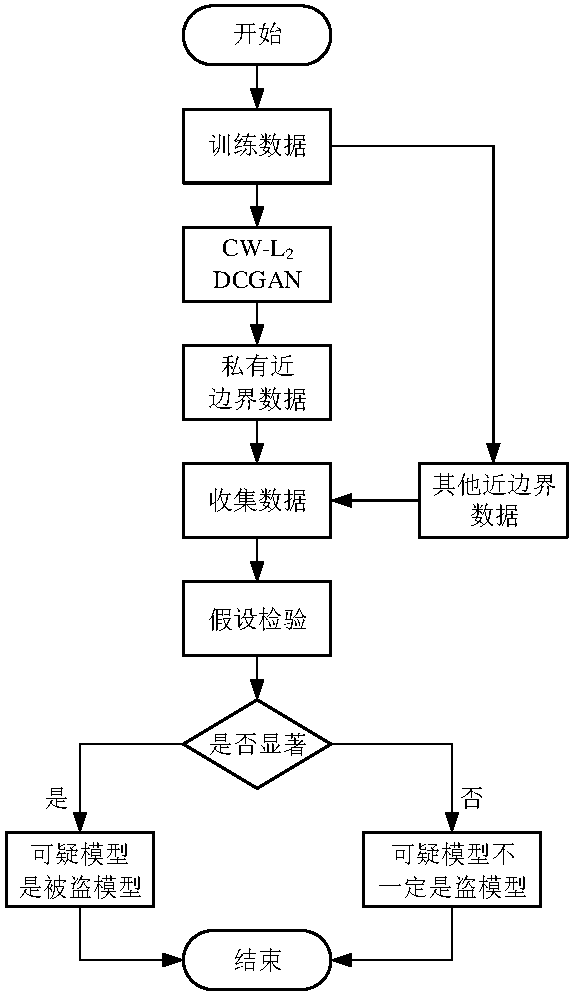
\includegraphics[width=0.50\linewidth]{方法整体流程图.pdf}
	\caption{方法整体流程图}
	\label{方法整体流程图}
	%	\vspace{-3mm}  %调整图片标题与下文距离,与\setlength{\belowcaptionskip}{-3mm}等效。
	\end {figure}
% !TeX root = ../main.tex
% -*- coding: utf-8 -*-

\chapter{基于近边界数据的模型所有权推断方法分析}\label{5}

本文在三个开源数据集上进行实验,选择ResNet18作为评估的源模型,VGG11作为对照的无关模型。本章将从初始近边界数据的生成算法、近边界数据私有化方法、近边界数据的可继承性、源模型微调的影响、模型所有权推断的有效性和近边界数据规模的可伸缩性这几个方面对本文提出的方法进行评估和分析。本文采用了几种主流的模型窃取攻击方法,包括模型微调,模型剪枝(不同的剪枝率)和模型知识蒸馏,并在源模型的基础上派生得到盗窃模型。

\section{实验设置}\label{5.1}

\subsection{数据集}

\noindent\textbf{CIFAR-10\cite{krizhevsky2009learning}:}CIFAR-10共有10个类别,其中训练集包含50000张大小为32x32的图像,测试集包含10000张大小为32x32的图像。

\noindent\textbf{Heritage\footnote{https://datahub.io/dataset/architectural-heritage-elements-image-dataset}:}Heritage共有10个类别,其中训练集包含10235张大小为128x128的图像,测试集包含1404张大小为64x64的图像。

\noindent\textbf{Intel\_image\footnote{https://www.kaggle.com/datasets/puneet6060/intel-image-classification}:}Intel\_image共有6个类别,其中训练集包含14034张大小为150x150的图像,测试集包含3001张大小为150x150的图像。

\subsection{实验环境和参数设置}

\textbf{(1)实验环境}

本文在实验中使用的硬件与软件配置如表\ref{table:11}所示,实验使用的机器配备16核Intel i7-11700KF CPU、NVIDIA GeForce RTX 3080 Ti显卡、16GB 内存以及Ubuntu 20.04 LTS操作系统,实验代码均使用Python语言和Pycharm工具基于Pytorch框架实现。

\begin{table}[H]
	\centering
%	\setlength{\arrayrulewidth}{0.5mm}
	\renewcommand\arraystretch{1.2}
	\caption{硬件与软件配置}
	\label{table:11}
	\small
	\begin{tabular*}{13cm}{@{\extracolsep{\fill}} l c }
%		\hline
		\toprule[1pt]
		\textbf{硬件/软件}      &   \textbf{配置}    \\
		\hline
%		\toprule[0.5pt]
		操作系统  &   Ubuntu 20.04 LTS    \\
		
		CPU     &   Intel Core i7-11700KF @ 3.6GHz       \\
		
		内存     &   16GB       \\
		
		显卡     &   NVIDIA GeForce RTX 3080 Ti \\
		
		CUDA版本     &   	11.6          \\
		
		深度学习框架     &   Pytorch 1.9.0          \\
		
		开发工具    &   Pycharm         \\
		
		开发语言     &   Python 3.7.11           \\
		
		\bottomrule[1pt]
%		\hline		
	\end{tabular*}
\end{table}

\textbf{(2)参数设置}

\textbf{源模型训练:}训练过程中使用Adam优化器并将学习率(Learning rate),训练轮次(Epoch)和每批次大小(Batch size)分别设置为0.0001,200和64,其他参数为默认值。

\textbf{模型蒸馏:}蒸馏模型实验选择从Resnet18蒸馏至VGG11,蒸馏时将蒸馏温度设置为20并且教师模型比例$\alpha$=0.7,训练过程中使用Adam优化器并将学习率,训练轮次和每批次大小分别设置为0.0001,20和64,其他参数为默认值。

\textbf{模型微调:}蒸馏模型实验选择固定模型其他层参数,重置全连接层参数进行微调,训练过程中使用Adam优化器并将学习率,训练轮次和每批次大小分别设置为0.0001,10和64,其他参数为默认值。

\textbf{模型剪枝:}分别以10\%,30\%,50\%的剪枝率对源模型权重进行剪枝,其他参数为默认值。

\textbf{初始近边界数据生成算法:}初始近边界数据生成采用改进的$CW$-$L_2$算法,选择有目标的生成方式,指定生成样本类别。训练过程中使用Adam优化器并将学习率,训练轮次和每批次大小分别设置为0.001,1000和64,,二分搜索次数设置为6,其他参数为默认值。

\textbf{近边界数据私有化方法:}私有近边界数据生成器采用DCGAN的基础结构,训练过程中使用Adam优化器并将学习率,训练轮次和每批次大小分别设置为0.0002,2000和64,其他参数为默认值。

本方法最后微调源模型阶段需要交替使用源模型损失函数和新设计的损失函数微调源模型,具体设置为10个轮次交替一次且交替次数最多为10次。

\subsection{源模型和盗窃模型}

本节模型训练过程中参数设置与上一小节保持一致。

\textbf{(1)源模型和无关模型}

本文的目标模型选用ResNet18网络架构,在上述三个数据集上分别进行训练,作为实验源模型,使用VGG11作为无关的对照模型。ResNet18和VGG11的参数信息如表\ref{table:10}所示。

\begin{table}[H]
	\centering
	%	\setlength{\arrayrulewidth}{0.5mm}
	\renewcommand\arraystretch{1.2}
	\caption{模型参数信息}
	\label{table:10}
	%	\zihaowu
	\small
	\begin{tabular*}{13cm}{@{\extracolsep{\fill}} l c c c }
%		\hline
		\toprule[1pt]
		\textbf{模型 }     &   \textbf{层数}    &   \textbf{计算量/亿}     &   \textbf{ 参数量/百万}     \\
		\hline
		
		ResNet18  &   18     &    9.559     &    11.670     \\
		
		VGG11     &   11     &    47.022    &    132.863     \\
		
		\bottomrule[1pt]
%		\hline		
	\end{tabular*}
\end{table}

本文在数据处理阶段将统一图片尺寸更改为64,为了更好的提取到图片中的特征,提高模型准确率,所以训练的时候将原始ResNet18中首层使用的7x7卷积核改成3x3,步长和填充随之改为1,并且舍弃最大池化层。

如表\ref{table:12}所示,更改结构后ResNet18在三个数据集上的准确率得到提升。其中,模型在CIFAR-10的准确率相较于其他两个数据集提升较大,因为CIFAR-10数据集本身的尺寸为32x32,是小尺寸图片。

\begin{table}[H]
	\centering
	%	\setlength{\arrayrulewidth}{0.5mm}
	\renewcommand\arraystretch{1.2}
	\caption{模型更改结构前后准确率对比}
	\label{table:12}
	%	\zihaowu
	\small
	\begin{tabular*}{13cm}{@{\extracolsep{\fill}} l c c c }
%		\hline
		\toprule[1pt]
		\textbf{数据集 }     &   \textbf{CIFAR-10}    &   \textbf{Heritage}     &   \textbf{Intel\_image}     \\
		\hline
		
		更改前准确率  &  0.853     &    0.862     &    0.848     \\
		
		更改后准确率 &   0.886     &    0.879    &    0.854     \\
		
		\bottomrule[1pt]
%		\hline		
	\end{tabular*}
\end{table}

更改结构后,ResNet18在三个数据集上的准确率与训练轮次的关系如图\ref{模型在三个数据集上的准确率}所示,基本在训练125次之后模型收敛,准确率基本维持不变。

\begin{figure}[htb]%%图,[htbp]是浮动格式
	\centering
	%	\setlength{\abovecaptionskip}{2mm} %图片标题与图片距离
	%	\vspace{-2mm}
	%	\setlength{\belowcaptionskip}{-3mm} %调整图片标题与下文距离
	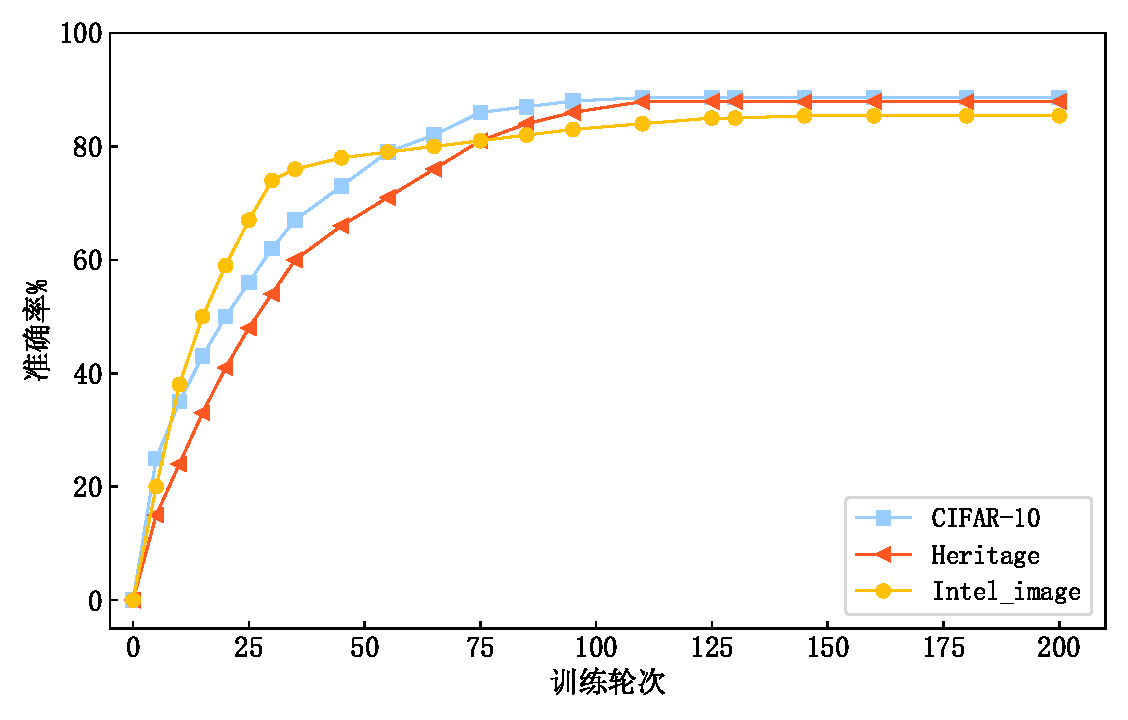
\includegraphics[width=0.9\linewidth]{准确率.pdf}
	\caption{源模型在三个数据集上的准确率}
	\label{模型在三个数据集上的准确率}
	%	\vspace{-3mm}  %调整图片标题与下文距离,与\setlength{\belowcaptionskip}{-3mm}等效。
	\end {figure}

\textbf{(2)盗窃模型}

\textbf{微调模型}:选择固定除全连接层外其余所有层的参数,将全连接层参数初始化后,进行微调作为盗窃模型。

\textbf{剪枝模型}:根据权重的$L_1$范数排序,对卷积层和全连接层分别以10\%,30\%,50\%的裁剪率进行裁剪作为盗窃模型。

\textbf{蒸馏知识}:选择蒸馏至VGG11作为盗窃模型,蒸馏时将蒸馏温度设置为20并且教师模型比例$\alpha$=0.7。
	
\section{初始近边界数据生成算法对比}\label{5.2}

本小节将对\ref{3}\ref{3.3}中提到的FGSM,IGSM,RFGSM和CW-$L_2$几种算法进行测试,评估指标为生成的初始近边界数据到分类边界的距离,距离愈小愈优。除对CW-$L_2$引入距离参数进行改进外,其余均使用原作者发布的实现。FGSM,IGSM,RFGSM中均有一个用于界定噪声$\epsilon$的参数,本文进行大量的实验探索选择合适的参数用于与CW-$L_2$进行比较。此外,CW-$L_2$的实验设置与第一节保持一致。

\begin{table}[H]
	\centering
%	\setlength{\arrayrulewidth}{0.5mm}
	\renewcommand\arraystretch{1.2}
	\caption{不同算法生成样本到分类边界的平均距离}
	\label{table:1}
	\small
	\begin{tabular*}{13cm}{@{\extracolsep{\fill}} l c c c c c}
		
%		\hline
		\toprule[1pt]
		\textbf{数据集}                 & \textbf{分组}  &   \textbf{FGSM}   &   \textbf{IGSM}   &  \textbf{RFGSM}  &   \pmb{CW-$L_2$}    \\
		\hline
\multirow{3}{6em}{CIFAR-10}    &1  &    0.557  &   0.430  &  0.418   &    \textbf{0.066}     \\
		                      & 2  &    0.461  &   0.419  &  0.373   &   \textbf{0.103}     \\
		                      & 3  &    0.586  &   0.369  &  0.356   &    \textbf{0.112 }    \\
		\hline
\multirow{3}{6em}{Heritage}   &  1 &    0.347  &   0.356  &  0.314   &    \textbf{0.014}     \\
		                      & 2  &    0.377  &   0.340  &  0.281   &    \textbf{0.016}     \\
		                      &  3 &    0.348  &   0.332  &  0.276   &    \textbf{0.010}     \\
		\hline
\multirow{3}{6em}{Intel\_image}& 1 &    0.522  &   0.447  &  0.353   &    \textbf{0.088}     \\
		                       & 2 &    0.475  &   0.506  &  0.387   &    \textbf{0.122}     \\
		                       & 3 &    0.468  &   0.402  &  0.428   &    \textbf{0.127}     \\
		\bottomrule[1pt]                      
%		\hline		
	\end{tabular*}
\end{table}

FGSM,IGSM,RFGSM和CW-$L_2$到分类边界的距离如表\ref{table:1}所示,每组测试下的最小距离已在表格中加粗。

从表中可以看出FGSM生成的样本效果较差,这是因为FGSM生成对抗性样本只进行一次噪声的添加,效率非常高。在追求效率的情况下,牺牲一定的性能是合理的。与FGSM相比,IGSM和RFGSM的效果稍好,因为这两种算法在执行过程中引入了迭代的步骤。通过每次迭代一小步,不断地在上一次的基础上添加噪声,使得图片以更小的幅度变化。这和表\ref{table:1}中的结果相符,即大部分情况下,IGSM和RFGSM的生成的对抗性样本到分类边界的平均距离比FGSM生成的样本更近。

经过改进后的CW-$L_2$算法在这几种方法中表现显著,相比其他三种方法,生成的对抗性样本到分类边界的距离小数十倍。这是因为该算法执行过程较为复杂,且速度较慢,在迭代过程中引入了二分查找和神经网络来训练参数以更好地生成对抗性样本。为进一步提升该算法的性能,本文在算法中引入了到分类边界距离这一参数,使得生成的对抗性样本更加接近分类边界,并在达到预定阈值$\theta$时提前终止算法,从而一定程度上缓解了效率低下的问题。

\section{近边界数据私有化方法对比}\label{5.3}

本小节将对\ref{4}\ref{4.1}中提到的BGAN,BEGAN和DCGAN三种生成对抗网络进行测试。与上一节一致,评估指标为训练收敛GAN后,生成器生成的新数据到目标分类边界的平均距离,距离愈小者愈优。

\begin{table}[H]
	\centering
	%	\setlength{\arrayrulewidth}{0.5mm}
	\renewcommand\arraystretch{1.2}
	\caption{不同GAN生成样本到分类边界的平均距离}
	\label{table:4}
	\small
	\begin{tabular*}{13cm}{@{\extracolsep{\fill}} l c c c c }
		\toprule[1pt]
		\textbf{数据集}      &  \textbf{分组}  &   \textbf{BGAN}   &   \textbf{BEGAN}   &  \textbf{DCGAN}  \\
		\hline
		\multirow{3}{6em}{CIFAR-10}    &1  &    0.189  &   0.212  &  \textbf{0.134}    \\
									&2	&    0.141  &   0.092  &  \textbf{0.072}   \\
									&3	&    0.187  &   \textbf{0.121}  &  0.210   \\
		\hline
		\multirow{3}{6em}{Heritage}   &  1 &    0.126  &   0.132  &  \textbf{0.097}    \\
										&2	&    0.221  &   0.167  &  \textbf{0.128}    \\
										&3	&    0.156  &   0.175  &  \textbf{0.144}    \\
		\hline
		\multirow{3}{6em}{Intel\_image}& 1 &    0.221  &   0.114  &  \textbf{0.042}   \\
									&2	&    0.088  &   0.263  &  \textbf{0.037}   \\
									&3	&    0.186  &   \textbf{0.103}  &  0.120   \\
		\bottomrule[1pt]	
	\end{tabular*}
\end{table}

BGAN,BEGAN和DCGAN生成的数据到分类边界的距离如表\ref{table:4}所示,每组测试下的最小距离已在表格中加粗。在大部分测试情况下,GCGAN生成的数据距离分类边界的距离最小。

BGAN和BEGAN都对原始GAN进行了改进,提升了生成图片的效果。在\ref{4}\ref{4.1}中,本文详细介绍了四点DCGAN相比于原有架构的改进。卷积对图像特征有着很强的处理能力,在这三种架构中,虽然BEGAN和DCGAN都是基于卷积神经网络的,但是实际测试中DCGAN的改进更加适配本文的数据。所以在本文的图像数据下,DCGAN表现出比其他两种网络结构更优秀的性能。因此,本文选择GCGAN来对初始的近边界数据进行特征提取,进而生成新的、私有化近边界数据。

\section{近边界数据的可继承性验证}\label{5.4}

本文提出的近边界数据不仅需要在源模型在表现出靠近分类边界的特点,而且在所有盗窃模型中也需要有这个性质。即近边界数据的近边界性可以继承到源模型派生出的模型上,这是本文选择近边界数据作为推断模型所有权的原因。本节将在三个数据集上,针对盗窃模型和无关模型,对不同目标分类边界下近边界数据的近边界性和可继承性进行测试与验证。每一组实验使用64个独立的私有近边界数据进行测试,针对3个数据集,每个数据集4条不同的分类边界,共16组测试。

\begin{figure}[!htb]
	\centering
%	\setlength{\abovecaptionskip}{0mm}
%		\vspace{-3mm}
%	\setlength{\belowcaptionskip}{-4mm} %调整图片标题与下文距离
	\subfigure{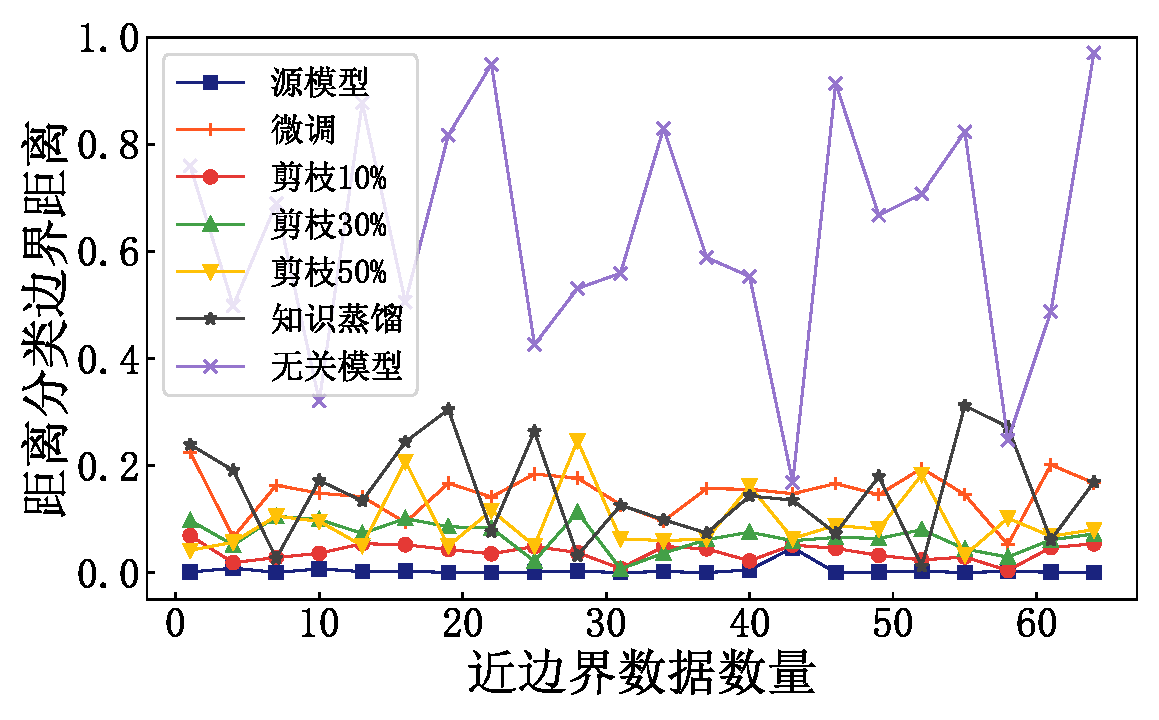
\includegraphics[width=0.49\linewidth]{CIFAR-10-4-2-distance.pdf}} 
	\subfigure{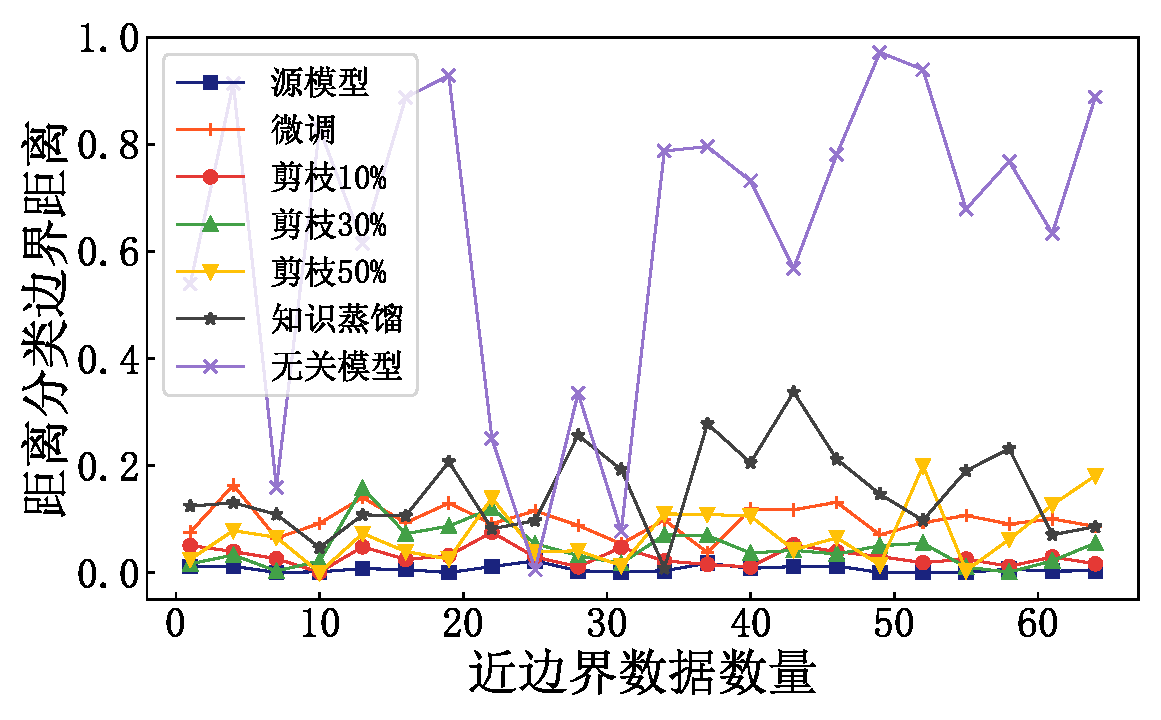
\includegraphics[width=0.49\linewidth]{CIFAR-10-4-3-distance.pdf}}
    \subfigure{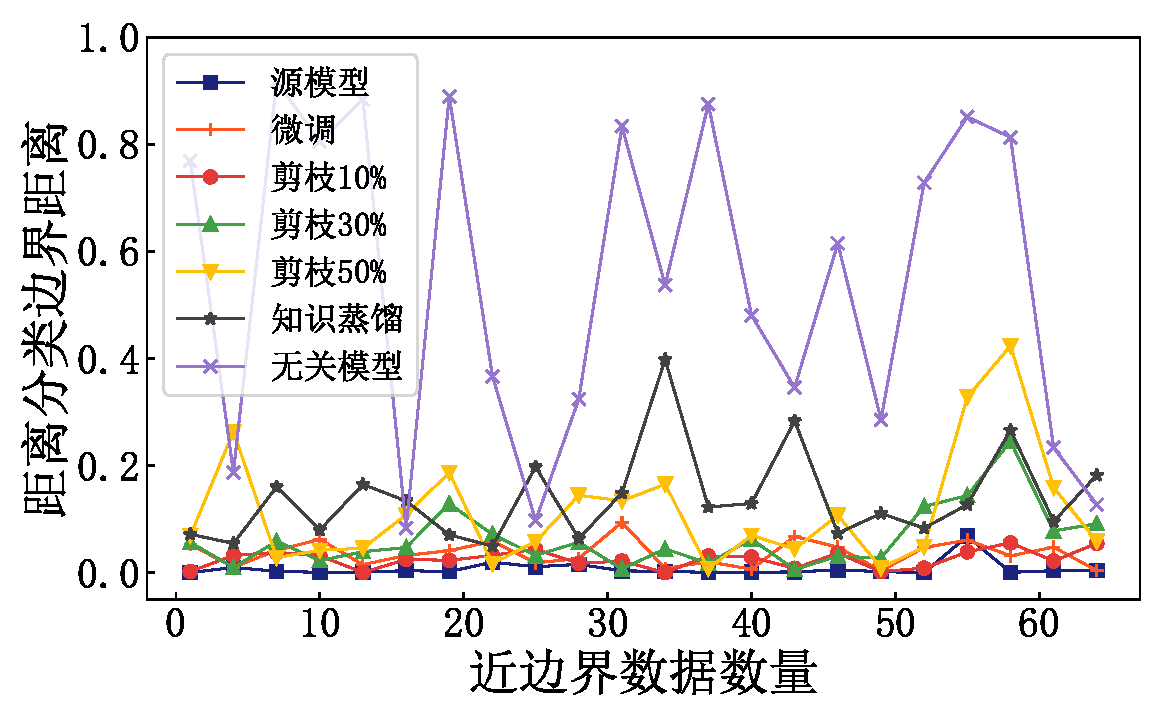
\includegraphics[width=0.49\linewidth]{CIFAR-10-4-7-distance.pdf}}
    \subfigure{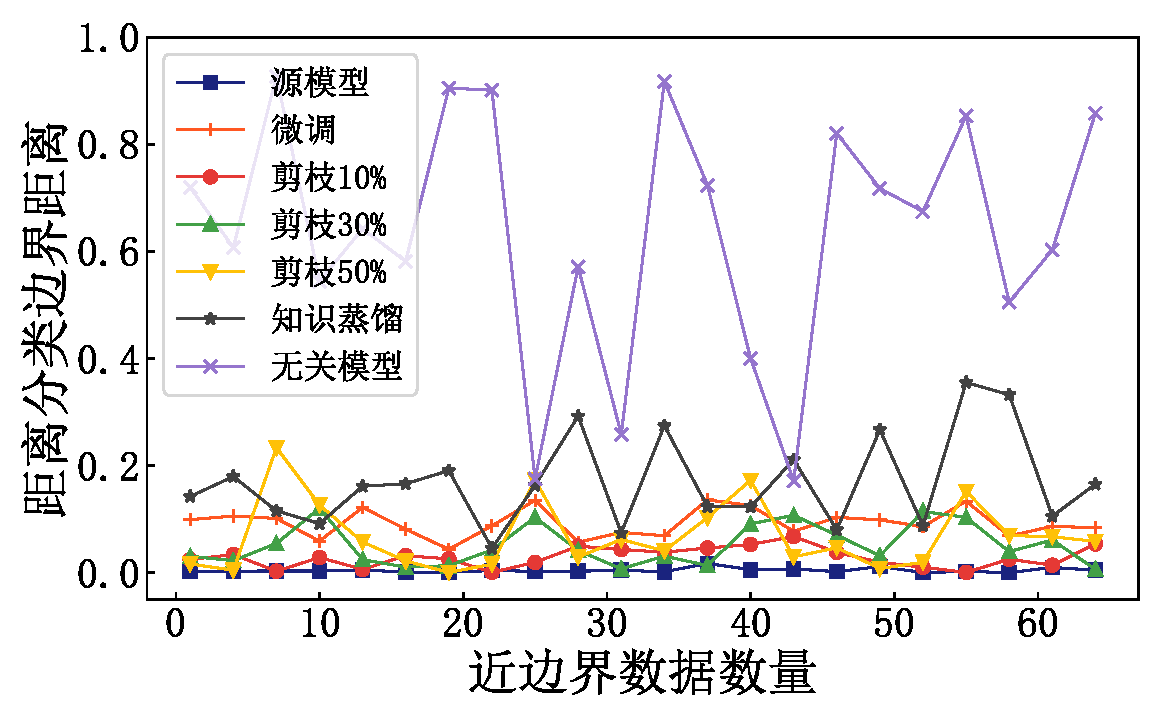
\includegraphics[width=0.49\linewidth]{CIFAR-10-5-6-distance.pdf}}
	\caption{CIFAR-10上4条不同分类边界下的近边界数据表现}
	\label{CIFAR-10上不同分类边界下的近边界数据表现}
\end{figure}

\begin{figure}[!htb]
	\centering
%	\setlength{\abovecaptionskip}{0mm}
%		\vspace{-3mm}
%	\setlength{\belowcaptionskip}{-4mm} %调整图片标题与下文距离
	\subfigure{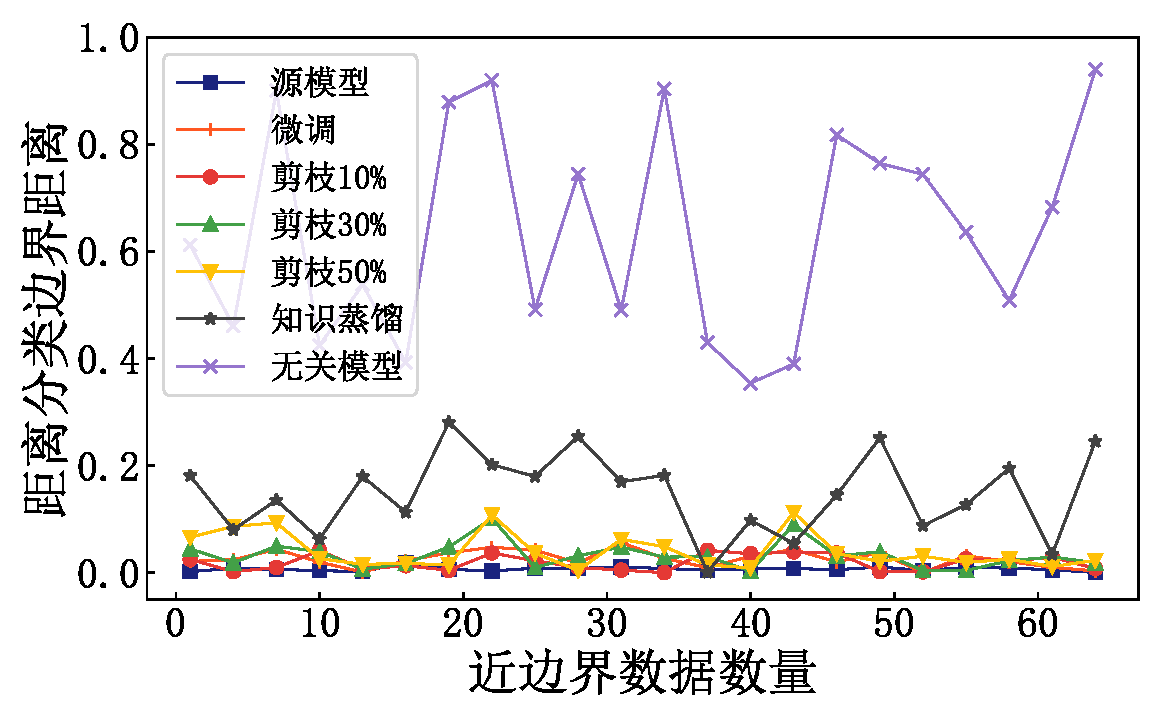
\includegraphics[width=0.49\linewidth]{Heritage-3-0-distance.pdf}} 
	\subfigure{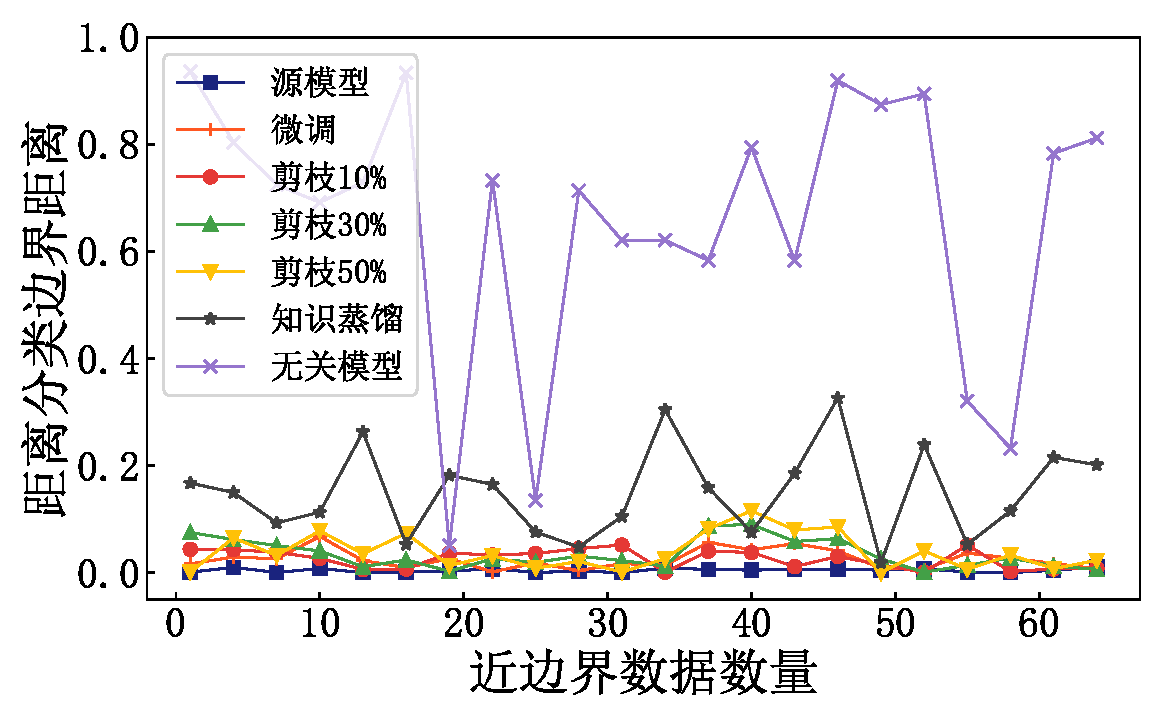
\includegraphics[width=0.49\linewidth]{Heritage-3-1-distance.pdf}} 
	\subfigure{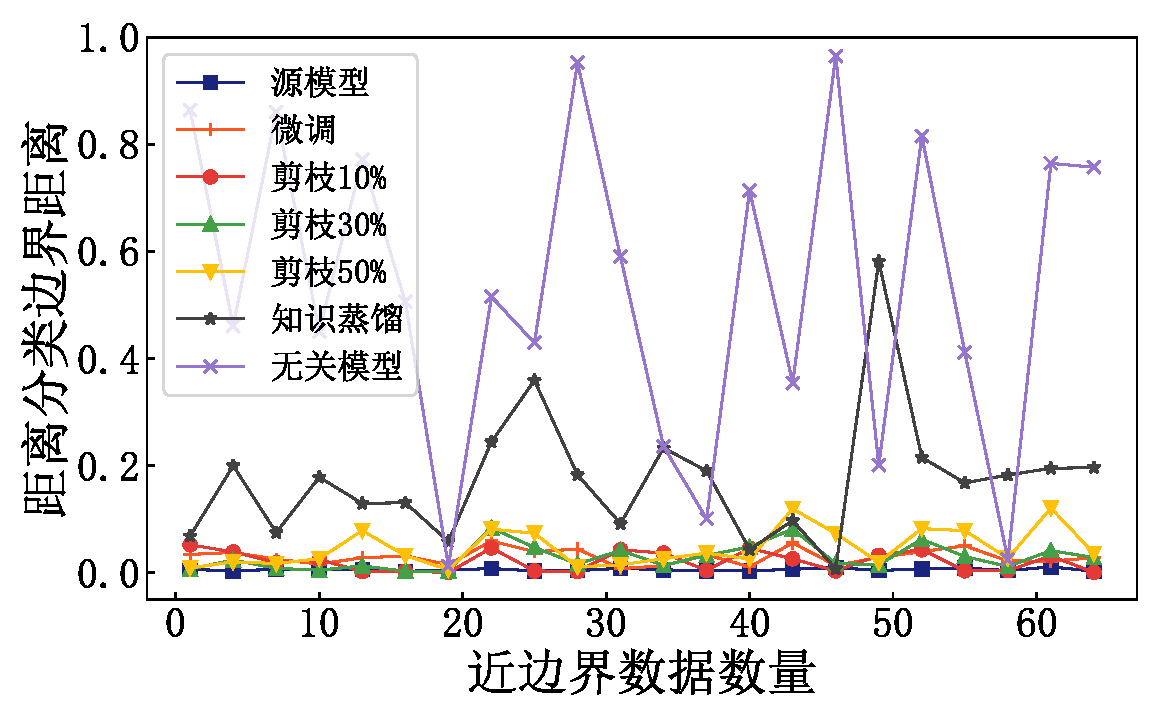
\includegraphics[width=0.49\linewidth]{Heritage-3-4-distance.pdf}} 
	\subfigure{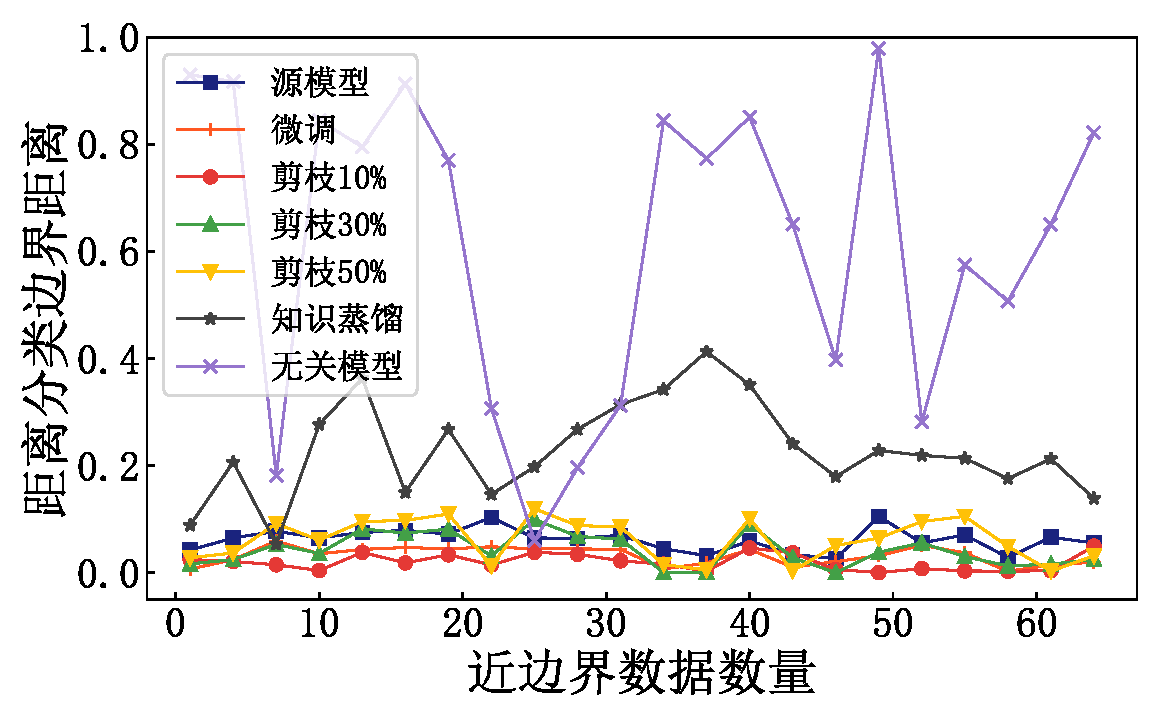
\includegraphics[width=0.49\linewidth]{Heritage-7-6-distance.pdf}} 
	\caption{Heritage上4条不同分类边界下的近边界数据表现}
	\label{Heritage上不同分类边界下的近边界数据表现}
\end{figure}

\begin{figure}[!htb]
	\centering
	\subfigure{\includegraphics[width=0.49\linewidth]{Intel\_image-3-1-distance.pdf}} 
	\subfigure{\includegraphics[width=0.49\linewidth]{Intel\_image-3-4-distance.pdf}} 
	\subfigure{\includegraphics[width=0.49\linewidth]{Intel\_image-3-5-distance.pdf}} 
	\subfigure{\includegraphics[width=0.49\linewidth]{Intel\_image-5-0-distance.pdf}}
	\caption{Intel\_image上4条不同分类边界下的近边界数据表现}
	\label{Intel-image上不同分类边界下的近边界数据表现}
\end{figure}

如图\ref{CIFAR-10上不同分类边界下的近边界数据表现},图\ref{Heritage上不同分类边界下的近边界数据表现},图\ref{Intel-image上不同分类边界下的近边界数据表现}所示, 本文提出的近边界数据在所有盗窃模型中都表现出了靠近分类边界的特点。从图中可以发现,相比于其他模型,近边界数据在源模型上距离分类边界的距离最近,这主要是三方面的原因:

1)初始的近边界样本是使用公开数据集在源模型的基础上生成的。本文从众多生成对抗性样本的方法中挑选了效果最好的CW-$L_2$方法,然后在该方法的基础上引入距离参数,改进算法的迭代过程,使之生成非常靠近目标分类边界的近边界数据。

2)使用DCGAN生成器提取近边界数据的特征后,生成了新的私有化近边界数据。在此基础上,本文设计了新的损失函数微调源模型分类边界,这使得私有近边界数据同样非常接近模型分类边界。

3)盗窃模型在从源模型派生的过程中,涉及到模型的修改。虽然这些修改操作不会使近边界数据在这些模型上失去近边界性,但是会使模型分类边界发生轻微偏移,从而近边界数据在盗窃模型上距离分类边界距离增大。


近边界数据在所有被盗模型中表现出近边界性说明近边界数据可以被继承,这跟本文使用的模型是DNN分类器有关。分类边界是分类器的重要特征,本文的近边界数据是根据分类边界构造的。即使模型窃取攻击对模型有一定程度的修改,分类器的分类边界不会发生很大的变化。因此,近边界数据拥有可继承性,在盗窃模型上同样表现出靠近分类边界的特点。这是本文提出方法的基础,因为本文方法的原理是,利用所有者的私有近边界数据和可疑对手提供的近边界数据到分类边界距离的大小来推断模型所有权(距离小者推断获得所有权)。如果私有近边界数据不表现出近边界性,那么就不适用于推断模型所有权。

从图中可以发现,相比于其他模型盗窃方法,近边界数据在知识蒸馏派生出的模型上距离分类边界距离较远。这是因为知识蒸馏对模型的修改特别大,通常来说会更换模型的架构,然后在通过蒸馏的方法进行训练。模型知识蒸馏对于其他模型知识产权保护方法也是一种挑战,但是本文提出的近边界数据在蒸馏产生的模型上仍然表现出近边界性,因此本文提出的方法对这种强修改的模型盗窃方法仍然适用。

图中还有一个点是近边界数据在无关模型上并不表现出近边界性,这是合理的。即使训练数据相同,分类边界不可能完全一样。本文提出的方法不应该对正常的无关模型产生误判,错误推断所有权。


\section{源模型微调的影响评估}\label{5.5}

本小节将对\ref{4}\ref{4.2}中使用私有近边界数据微调源模型产生的影响进行评估。本文针对不同数据集训练得到的源模型,使用不同规模的近边界数据以及不同的目标分类边界对源模型进行微调。评估指标为模型的准确率,准确率变化愈小,说明产生的不良影响越小。

\begin{table}[h]
	\centering
	%	\setlength{\arrayrulewidth}{0.5mm}
	\renewcommand\arraystretch{1.2}
	\caption{微调分类边界对准确率的影响}
	\label{table:3}
%	\resizebox{\linewidth}{!}{
%		\zihaowu
	\small
	\begin{tabular*}{14cm}{@{\extracolsep{\fill}} l c c c c}
		\toprule[1pt]
		\multirow{3}{5em}{分类边界}&\multirow{3}{5em}{数据规模} & CIFAR-10&Heritage&Intel\_image \\ 
		& & 准确率(0.886)&准确率(0.879)&准确率(0.854) \\
		\cline{3-5}	
		& &准确率&准确率&准确率 \\
		\hline
		\multirow{4}{5em}{分类边界1}&64&0.873&0.862&0.825 \\
		&128&0.862&0.858&0.829 \\
		&256&0.862&0.854&0.826 \\
		&512&0.857&0.852&0.839 \\
		\hline
		\multirow{4}{5em}{分类边界2}&64&0.871&0.867&0.843 \\
		&128&0.870&0.862&0.839 \\
		&256&0.860&0.859&0.828 \\
		&512&0.859&0.851&\textbf{0.824} \\
		\hline
		\multirow{4}{5em}{分类边界3}&64&0.871&0.865&0.841 \\
		&128&0.868&0.857&0.833 \\
		&256&0.858&0.855&0.831 \\
		&512&\textbf{0.856}&0.851&0.825 \\
		\hline
		\multirow{4}{5em}{分类边界4}&64&0.873&0.863&0.847 \\
		&128&0.873&0.860&0.843 \\
		&256&0.866&0.854&0.838 \\
		&512&0.862&\textbf{0.850}&0.831 \\
		\hline
		\multirow{4}{5em}{分类边界5}&64&0.876&0.866&0.846 \\
		&128&0.866&0.861&0.834 \\
		&256&0.868&0.857&0.829 \\
		&512&0.861&0.853&0.825 \\
		\bottomrule[1pt]
\end{tabular*}
%}
\end{table}

	
经过不同规模近边界数据微调后,源模型的准确率如表\ref{table:3}所示,每个数据集下影响最大,即准确率最低的,已在表中加粗。

从表中可以发现,几乎全部情况下,源模型微调前后的精度差没有超过3\%,这是本文方法可以接受的范围。不考虑偶然因素的影响,在大部分情况下,随着微调模型近边界数量的增多,模型准确率逐渐下降。这是合理的,因为近边界数据本身和正常训练数据不同,使用越多的异常数据参与训练,对模型的性能影响越大。但是在另一个角度,微调源模型的目的是使得私有近边界数据更加靠近目标分类边界,来提高后续推断模型所有权的置信度,所以,使用更多的近边界数据微调源模型,后续推断的效果会更好。因此,在实际情况中,微调数据规模的选择是一个模型精度和推断置信度的折衷。

表中整体情况下,模型的准确率下降不多。一方面,这是因为微调的数据和源模型的训练数据相比只是一小部分,不会对模型产生太大的影响。另一方面,在微调源模型时,本文将学习率设置较低,仅为0.0001。并且使用原始数据对模型进行交替训练,训练轮次不超过10次。所以对源模型微调之后,模型准确率没有受到很大的影响。

实验结果证明,本文的私有近边界数据在解决模型所有权保护问题时,模型具有较好的保真度。因此,使用近边界数据推断模型所有权不用担心源模型受到较大的影响,模型准确率变化在3\%以内。	
	

\section{模型所有权推断有效性评估}\label{5.6}

本文提出的方法目标是推断模型的所有权,本节将对此方法的有效性进行评估。根据本文方法的流程,模型所有者和可疑对手(可能是模型盗窃者)均需向官方仲裁机构提供各自的近边界数据,然后通过数据和模型计算到分类边界的距离,再根据\ref{4}\ref{4.3}中提到的假设检验进行进行结果对比,判断可疑模型是否从源模型派生。

在本节中,通过讨论本文方法生成的私有近边界数据与其他近边界数据在盗窃模型上的性能对比来说明本文方法的有效性。首先,本文模拟了盗窃者可能会提供的近边界数据,该数据由两部分组成,包括(1)从原始数据中挑选出的近边界数据,(2)由FGSM和CW生成的一些对抗性样本。然后针对不同的目标分类边界,进行假设检验并计算在不同数据集和不同盗窃模型上的$\Delta\mu$和$p$值,来反映成功推断所有权的置信度。本节的评估指标为$\Delta\mu$和$p$值,$\Delta\mu$愈大和$p$值愈小,推断的置信度愈高。

\begin{table}[h]
	\centering
%	\setlength{\arrayrulewidth}{0.5mm}
	\renewcommand\arraystretch{1.5}
	\caption{推断模型所有权}
	\label{table:2}
	\resizebox{\linewidth}{!}{
	\begin{tabular}{l l c c c c c c c c c c}
		
		\toprule[1pt]
\multirow{2}{5em}{数据集}&\multirow{2}{4em}{攻击方法}&\multicolumn{2}{c}{分类边界1}&\multicolumn{2}{c}{分类边界2}&\multicolumn{2}{c}{分类边界3}&\multicolumn{2}{c}{分类边界4}&\multicolumn{2}{c}{分类边界5}\\ \cline{3-12}
		                         & &$\Delta\mu$&$p$值&$\Delta\mu$&$p$值&$\Delta\mu$&$p$值&$\Delta\mu$&$p$值&$\Delta\mu$&$p$值 \\
		\hline
\multirow{6}{5em}{CIFAR-10}     &源模型    & 0.913 & $10^{-6}$ & 0.954 & $10^{-6}$ & 0.927 & $10^{-5}$ & 0.967 & $10^{-5}$ & 0.958 & $10^{-5}$   \\
								&模型微调  & 0.718 & $10^{-5}$ & 0.745 & $10^{-6}$ & 0.698 & $10^{-5}$ & 0.692 & $10^{-4}$ & 0.729 & $10^{-5}$   \\
								& 剪枝10\% & 0.572 & $10^{-5}$ & 0.487 & $10^{-5}$ & 0.458 & $10^{-5}$ & 0.533 & $10^{-4}$ & 0.512 & $10^{-4}$   \\
								&剪枝30\%  & 0.537 & $10^{-4}$ & 0.497 & $10^{-4}$ & 0.401 & $10^{-3}$ & 0.428 & $10^{-4}$ & 0.587 & $10^{-4}$   \\
								&剪枝50\%  & 0.545 & $10^{-4}$ & 0.614 & $10^{-4}$ & 0.506 & $10^{-3}$ & 0.570 & $10^{-4}$ & 0.484 & $10^{-3}$   \\
								&知识蒸馏  & 0.372 & $10^{-3}$ & 0.297 & $10^{-3}$ & 0.288 & $10^{-3}$ & 0.308 & $\pmb{10^{-2}}$ & 0.340 & $10^{-3}$   \\
		\hline
\multirow{6}{5em}{Heritage}     &源模型    & 0.876 & $10^{-5}$ & 0.845 & $10^{-5}$ & 0.859 & $10^{-4}$ & 0.801 & $10^{-4}$ & 0.837 & $10^{-5}$   \\
								&模型微调  & 0.815 & $10^{-5}$ & 0.792 & $10^{-4}$ & 0.824 & $10^{-4}$ & 0.833 & $10^{-4}$ & 0.784 & $10^{-4}$   \\
								&剪枝10\%  & 0.530 & $10^{-4}$ & 0.535 & $10^{-3}$ & 0.508 & $10^{-4}$ & 0.486 & $10^{-3}$ & 0.471 & $10^{-3}$   \\
								&剪枝30\%  & 0.491 & $10^{-3}$ & 0.452 & $10^{-3}$ & 0.469 & $10^{-4}$ & 0.470 & $10^{-3}$ & 0.427 & $10^{-4}$   \\
								&剪枝50\%  & 0.502 & $10^{-3}$ & 0.517 & $10^{-3}$ & 0.434 & $10^{-3}$ & 0.451 & $10^{-3}$ & 0.490 & $10^{-3}$   \\
								&知识蒸馏  & 0.329 & $10^{-3}$ & 0.365 & $\pmb{10^{-2}}$ & 0.238 & $10^{-3}$ & 0.310 & $10^{-3}$ & 0.274 & $10^{-3}$   \\
		\hline
\multirow{6}{5em}{Intel\_image} &源模型    & 0.859 & $10^{-5}$ & 0.896 & $10^{-4}$ & 0.872 & $10^{-4}$ & 0.899 & $10^{-4}$ & 0.914 & $10^{-4}$   \\
								&模型微调  & 0.717 & $10^{-5}$ & 0.784 & $10^{-4}$ & 0.752 & $10^{-4}$ & 0.791 & $10^{-3}$ & 0.709 & $10^{-4}$   \\
								&剪枝10\%  & 0.451 & $10^{-4}$ & 0.522 & $10^{-4}$ & 0.539 & $10^{-3}$ & 0.472 & $10^{-3}$ & 0.438 & $10^{-4}$   \\
								&剪枝30\%  & 0.407 & $10^{-4}$ & 0.415 & $10^{-4}$ & 0.346 & $10^{-3}$ & 0.382 & $10^{-3}$ & 0.395 & $10^{-3}$   \\
								&剪枝50\%  & 0.370 & $10^{-3}$ & 0.395 & $10^{-3}$ & 0.327 & $10^{-3}$ & 0.360 & $10^{-3}$ & 0.458 & $10^{-3}$   \\
								&知识蒸馏  & 0.336 & $\pmb{10^{-2}}$ & 0.395 & $10^{-3}$ & 0.360 & $\pmb{10^{-2}}$ & 0.308 & $10^{-3}$ & 0.287 & $\pmb{10^{-2}}$   \\
		\bottomrule[1pt]		
	\end{tabular}
}
\end{table}

不同数据集下,针对不同分类边界,所有者的私有近边界数据和其他近边界数据计算得到的$\Delta\mu$和$p$值如表\ref{table:2}所示,不同目标分类边界下$p$值的最小情况已在表格中加粗。

从表中可以发现,在每个数据集,每条分类边界上$p$值呈从上到下增大的趋势,$\Delta\mu$呈减小趋势。尽管如此,在全部情况中,$p$值均低于0.05,即至少有95\%以上的置信度,推断盗窃模型从源模型派生。即本文的方法在不同的模型窃取方法中推断模型的所有权,均有显著的效果,至少有95\%以上的置信度确定可疑模型是盗窃模型。

在假设检验中,$p$值越小,$\Delta\mu$越大说明结果越可靠,推断的置信度越高。表中从上到小$p$值减小是因为这些模型窃取方法对模型的修改逐渐增大,尤其是知识蒸馏。模型知识蒸馏是本文方法的最大挑战,也同样是其他研究面临的巨大挑战。从表中,可以观察到本文提出的的方法始终可以将蒸馏模型推断为被盗模型。因此,实验结果表明使用私有的近边界数据来推断模型所有权的方法对大多数模型盗窃技术都是可靠的,模型被盗窃的置信度至少达到95\%,证明了本文方法的有效性和鲁棒性。


\section{近边界数据规模可伸缩性评估}\label{5.7}

本节将测试使用不同规模的近边界数据,在推断模型所有权时的可伸缩性。本文提出的方法需要对数据进行采样从而进行假设检验,通常情况下,样本数量越大,检验过程中因随机因素而产生的不利影响就会越小,更能准确的推断可疑模型所有权。

\begin{figure}[!htb]
	\centering
	\subfigure{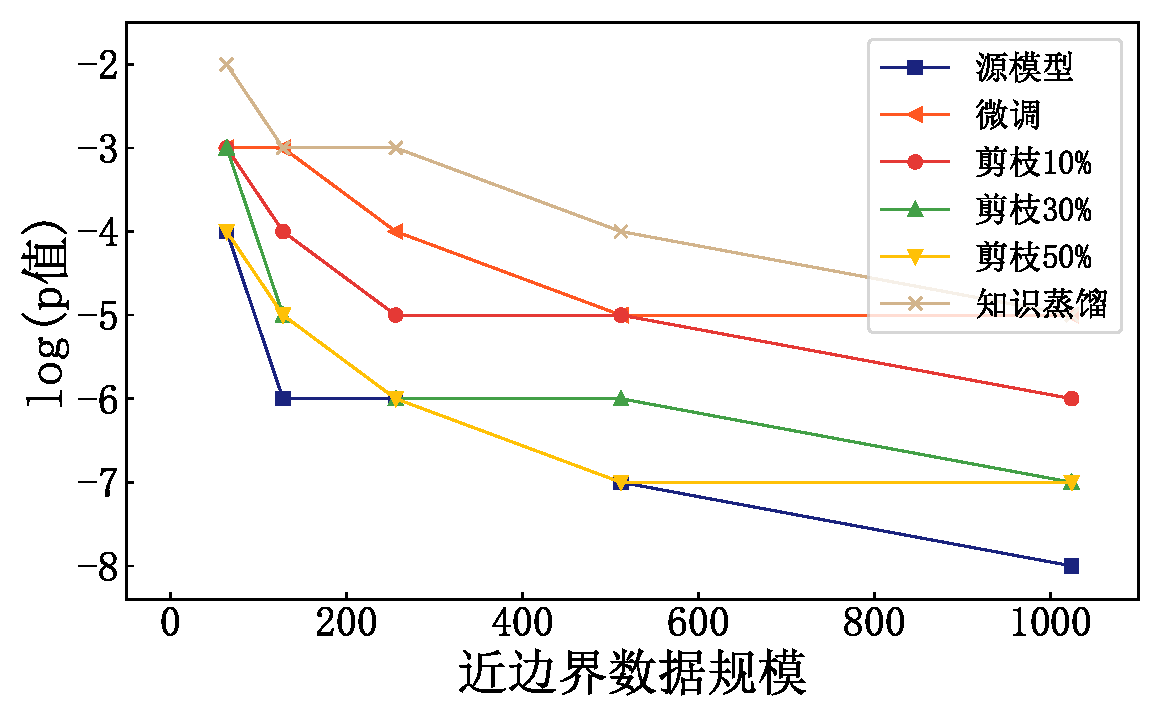
\includegraphics[width=0.49\linewidth]{CIFAR-10-4-2-p-value.pdf}} 
	\subfigure{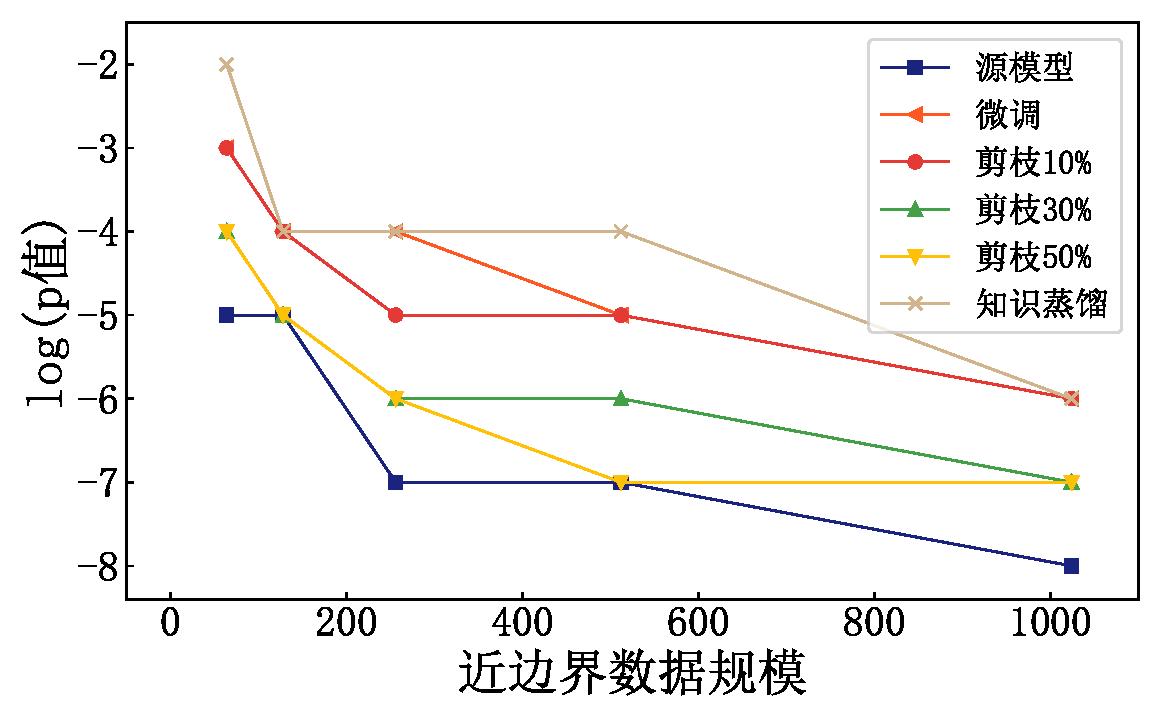
\includegraphics[width=0.49\linewidth]{CIFAR-10-4-3-p-value.pdf}}
	\subfigure{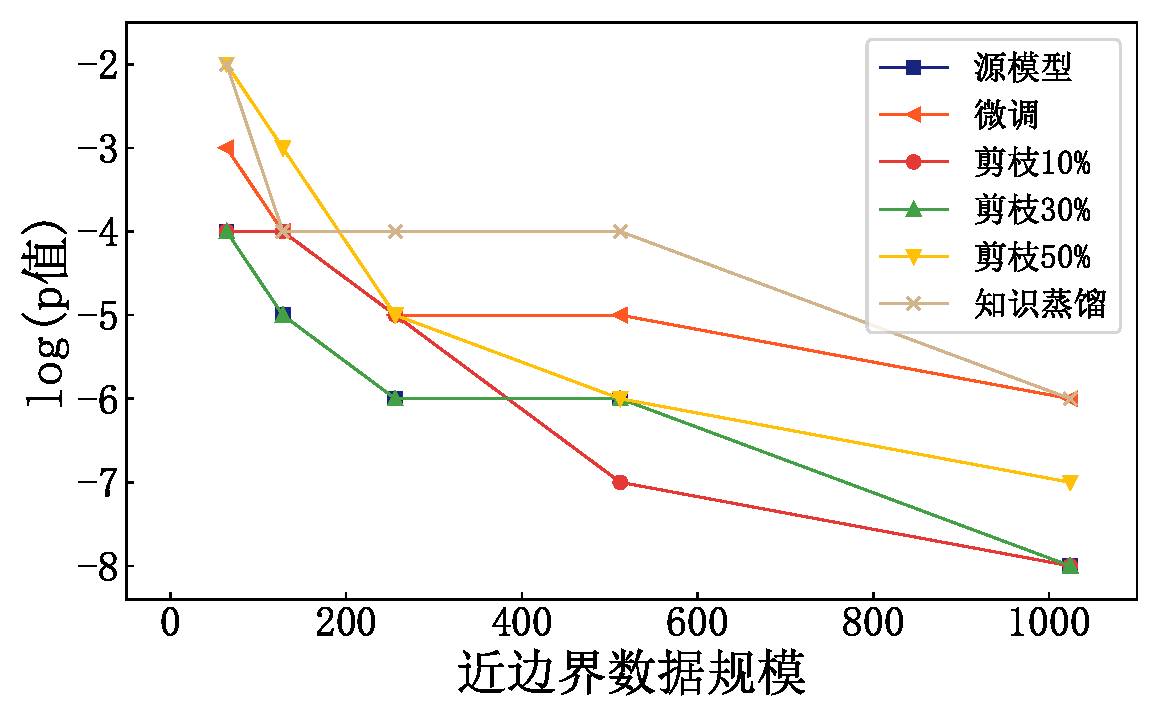
\includegraphics[width=0.49\linewidth]{CIFAR-10-4-7-p-value.pdf}}
	\subfigure{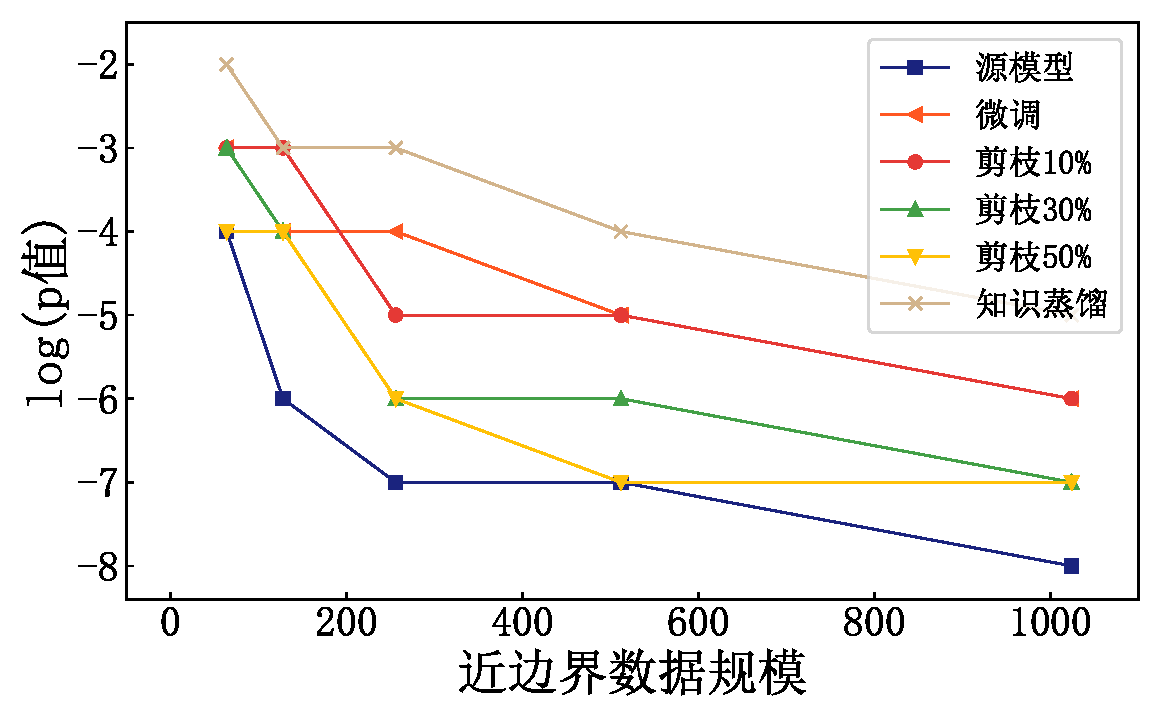
\includegraphics[width=0.49\linewidth]{CIFAR-10-5-6-p-value.pdf}} 
	\caption{CIFAR-10上4条不同分类边界下的近边界数据规模可伸缩性}
	\label{CIFAR-10上推断模型所有权的扩展性}
%	\setlength{\abovecaptionskip}{7mm}
\end{figure}

\begin{figure}[!htb]
	\centering
	\subfigure{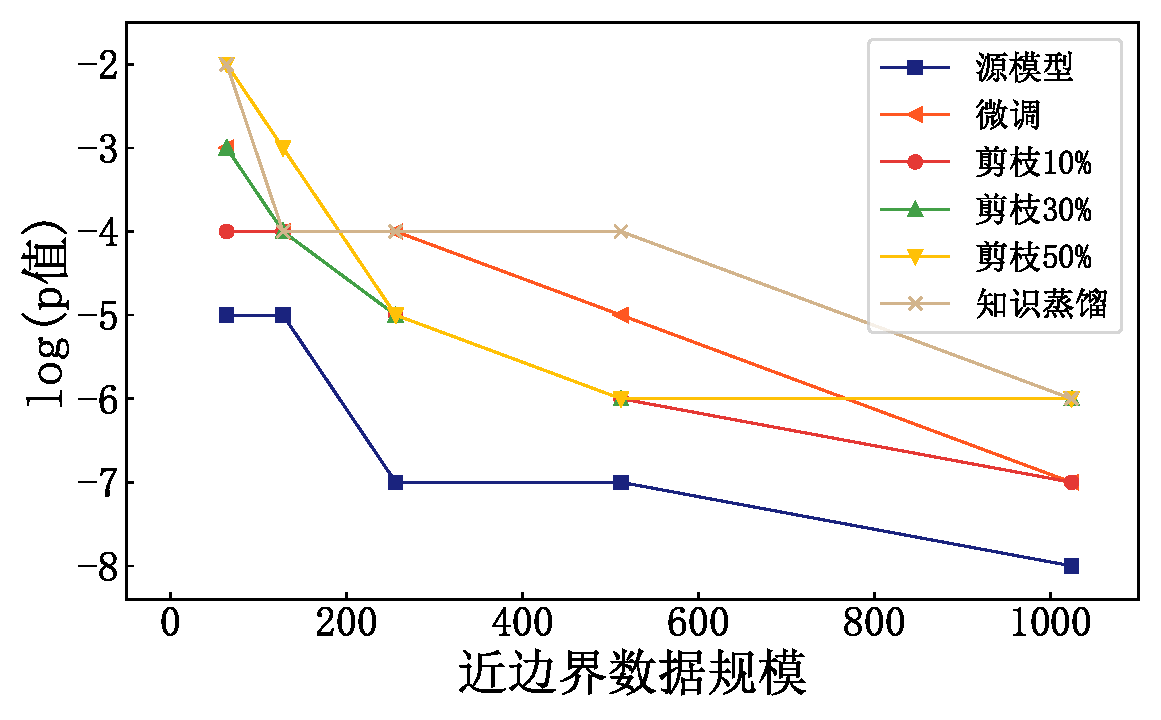
\includegraphics[width=0.49\linewidth]{Heritage-3-0-p-value.pdf}} 
	\subfigure{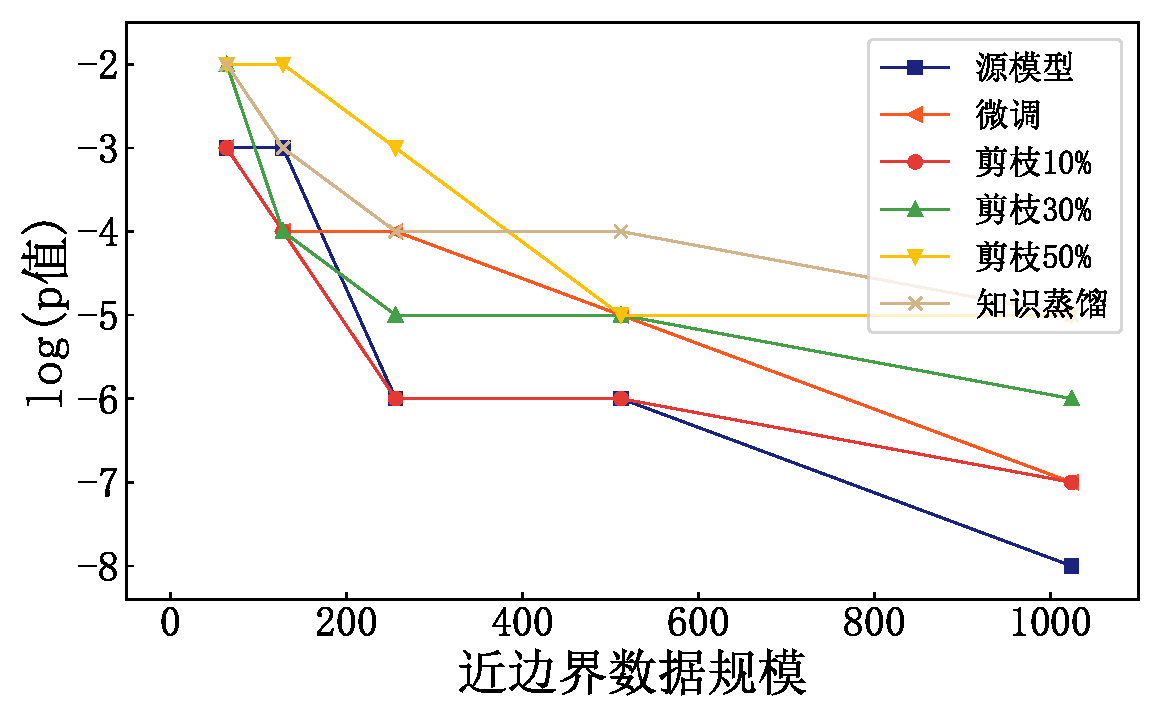
\includegraphics[width=0.49\linewidth]{Heritage-3-1-p-value.pdf}} 
	\subfigure{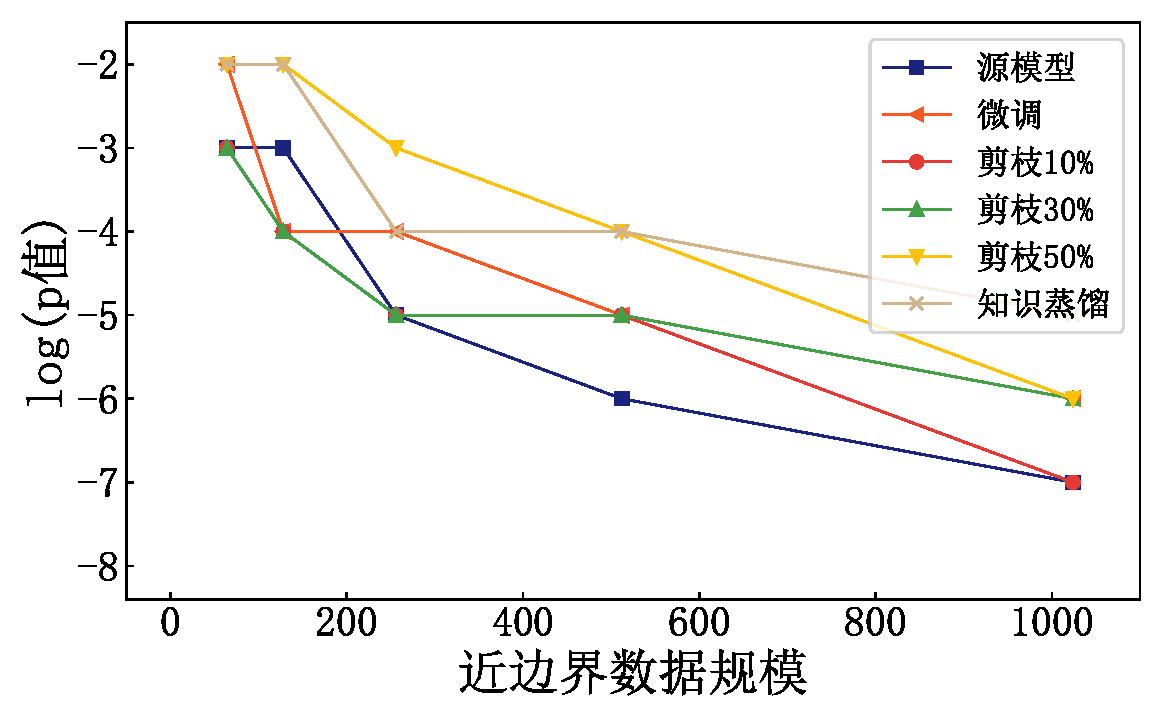
\includegraphics[width=0.49\linewidth]{Heritage-3-4-p-value.pdf}} 
	\subfigure{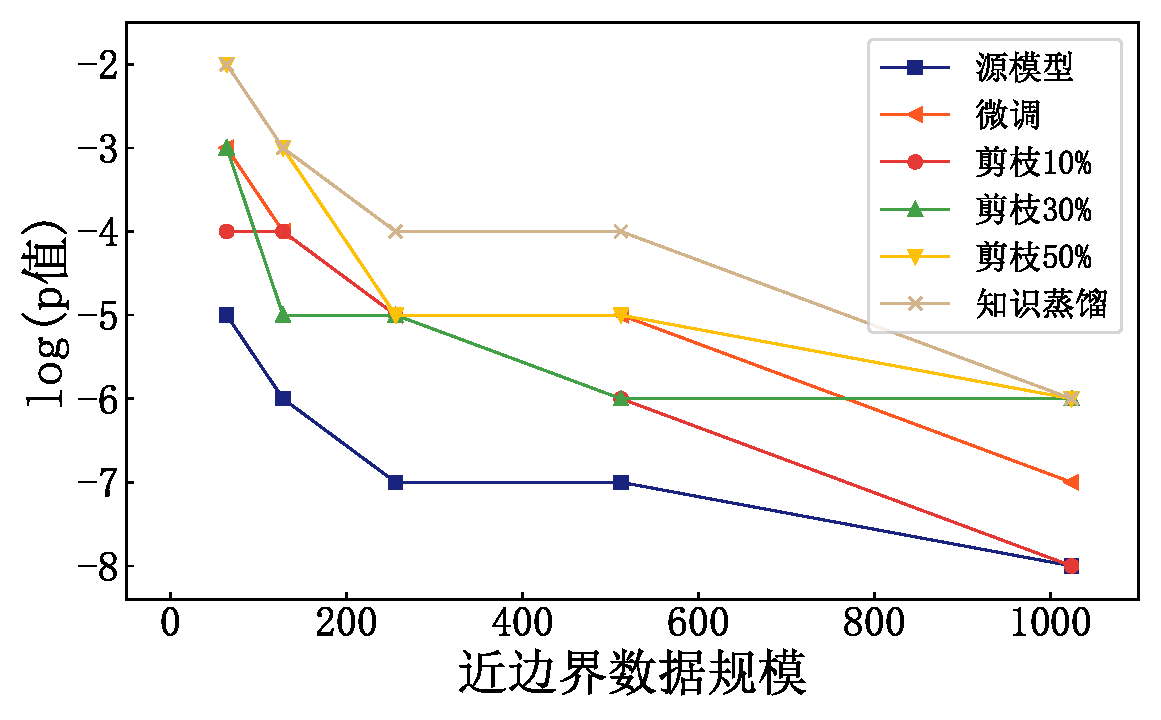
\includegraphics[width=0.49\linewidth]{Heritage-7-6-p-value.pdf}} 
	\caption{Heritage上4条不同分类边界下的近边界数据规模可伸缩性}
	\label{Heritage上推断模型所有权的扩展性}
%	\setlength{\abovecaptionskip}{7mm}
\end{figure}

\begin{figure}[!htb]
	\centering
	\subfigure{\includegraphics[width=0.49\linewidth]{Intel\_image-3-1-p-value.pdf}} 
	\subfigure{\includegraphics[width=0.49\linewidth]{Intel\_image-3-4-p-value.pdf}} 
	\subfigure{\includegraphics[width=0.49\linewidth]{Intel\_image-3-5-p-value.pdf}} 
	\subfigure{\includegraphics[width=0.49\linewidth]{Intel\_image-5-0-p-value.pdf}} 
	\caption{Intel\_image上4条不同分类边界下的近边界数据规模可伸缩性}
	\label{Intel-image上推断模型所有权的扩展性}
%	\setlength{\abovecaptionskip}{7mm}
\end{figure}

如图\ref{CIFAR-10上推断模型所有权的扩展性},图\ref{Heritage上推断模型所有权的扩展性},图\ref{Intel-image上推断模型所有权的扩展性}所示,$p$值在不同数据集,不同分类边界上,随着近边界数据规模的增大而减小,而$p$值越小说明假设检验能够以更高的置信度确定可疑模型是被盗模型。

本文的方法在进行假设检验前,需要将私有的近边界数据和可疑对手的近边界数据分别通过可疑模型,计算到目标分类边界的距离。可疑对手的近边界数据是通过从原始数据挑选和FGSM,CW生成的对抗性样本组成的。因此,由于随机因素的影响,存在一小部分可疑对手提供的数据到分类边界的距离和所有者提供的私有近边界数据相近,甚至更小的情况,这会对本文的方法产生一定的干扰。随着测试样本规模的增大,这种随机因素的影响会被逐渐消除。从图中可以发现,随着近边界数据规模的增大,$p$值逐渐减小。但这并不说明本文的方法对小规模数量的近边界数据缺少鲁棒性,从图中可以发现,即使在数据量为64的情况下,$p$值仍然小于0.05,这证明本文的方法对于小数样本量同样有显著的效果,可以高置信度的推断模型所有权。\\

\textbf{方法设计目标分析}

以下对\ref{4}\ref{4.3}中提出的方法设计目标进行分析。

1)\textbf{精确性:}本文方法对模型精确性的影响主要来源于使用近边界数据微调源模型目标分类边界,这是为了增加推断模型所有权的置信度。\ref{5.5}评估了不同规模近边界数据微调源模型的影响,各种情况下,模型精度下降不超过3\%。

2)\textbf{可继承性:}\ref{5.4}中通过16组测试,验证了近边界数据的可继承性,这是选择近边界数据进行所有权推断的原因。另外,无关模型没有对近边界数据没有表现出明显特征,表明本文的方法不会产生误判。

3)\textbf{有效性:}\ref{5.6}中,使用私有近边界数据和其他近边界数据,针对各种盗窃模型,计算距离结果。然后对双方的结果进行假设检验,结果表明了本文的方法推断所有权的有效性。此外,与过去工作中利用模型水印和指纹验证模型所有权相比,本文方法使用数据在对应模型上结果作为所有权推断依据,结果的可比性和唯一性可以有效避免歧义攻击。

4)\textbf{鲁棒性:}\ref{5.4}和\ref{5.6}中,对各种盗窃模型进行了测试,本文的方法均有效,表明了本文方法的鲁棒性。

5)\textbf{不可获得性:}本文使用改进的CW-$L_2$构造了初始近边界数据,并且设计了基于DCGAN的特征提取器,私有化近边界数据。模型盗窃者由于不知道约定的分类边界,需要大量的测试,这会导致极大的成本代价。不存在无法攻击的防御方法,但可以从攻击成本上进行约束。

6)\textbf{高效性:}本文方法使用模型所有者和盗窃者提供的近边界数据输入模型后计算结果,然后通过假设检验的方式对比结果差异。该过程执行方便,不涉及复杂的处理,可以高效的进行。

\section{本章小结}

本章在CIFAR-10,Heritage,Intel\_image这三个数据集上对本文提出的方法进行了全面的测评与分析。第二节,对不同初始近边界数据生成算法进行对比,结果表明CW-$L_2$方法可以满足本文的需求,生成足够靠近目标分类边界的近边界数据。第三节,对近边界数据私有化方法进行了对比,结果表明基于DCGAN的网络架构可以更好的提取数据样本特征,生成新的靠近分类边界的数据。第四节,通过16组测试验证了近边界数据的可继承性,这是本文方法选择近边界数据作为推断数据的原因。第五节,测试了微调分类边界对模型准确率的影响,保护模型知识产权的方法不应该对模型精度造成很大的影响,否则该方法失去了意义。第六节,评估了本文方法推断模型所有权的有效性,结果表明该方法对不同的模型盗窃方法均能以95\%以上的置信度推断可疑模型是盗窃模型。第七节,对假设检验的样本规模进行了扩展,在更大规模的情况下,本文的方法会更加有效,当然,该方法也适用于类似64的小样本数据情况。

% !TeX root = ../main.tex
% -*- coding: utf-8 -*-
\chapter{总结与展望}\label{6}

本章对本文提出的基于近边界数据的模型所有权推断方法进行总结,主要包括研究背景、存在问题,实现方案以及主要贡献。然后通过分析方法的不足之处,提出对未来工作的展望。

\section{工作总结}

随着科技的不断发展,深度神经网络模型逐渐成熟,并在社会发展中扮演着日益重要的角色。然而,由于训练成熟、高性能的DNN模型需要昂贵的成本,不法分子开始对这些模型发起窃取攻击,带来了严重的知识产权问题。

本文主要针对神经神经网络模型的知识产权保护方法进行研究。模型水印和模型指纹是目前解决模型知识产权问题的两种主要方法,通过相关工作的调研发现,这两种方法在验证模型所有权时很难抵御歧义攻击。针对上述问题,本文提出了使用数据驱动推断模型所有权,代替传统验证所有权的新思路。本文认为可以从数据驱动的角度抵御模型盗窃,即在源模型上找到一种可以量化的属性,如果这种属性会被源模型派生出的模型所继承,那么就可以从这个角度设计算法来推断模型的所有权。根据这个思想,本文构造了一类特殊的数据——近边界数据,作为推断所有权的依据。本文的主要贡献如下:

1)提出基于数据推断所有权代替验证所有权,解决验证所有权带来的歧义攻击问题。推断模型所有权是比较某类数据在模型上的最优性,最优者推断获得该模型的所有权。这种方式并不是去验证特定的水印或指纹,结果的可比性和唯一性可以有效避免歧义攻击。

2)提出近边界数据这一特殊数据,作为推断模型所有权的依据。本文基于三个公开数据集在盗窃模型和无关模型上做了充分的测试,验证了近边界数据的近边界性可以被盗窃模型所继承,而在无关模型上不会有近边界的特点,因此可以作为推断所有权的依据。利用对抗性样本靠近模型分类边界的特点,在CW-$L_2$算法的基础上,实现本文生成初始近边界数据的算法。实验表明此算法生成的数据足够靠近分类边界,满足推断所有权的要求。

3)对近边界数据进行私有化处理并基于处理后的数据对源模型进行微调,针对各种模型盗窃技术增强本文方法的性能和防御性。为了防止近边界数据被轻易伪造,设计了基于DCGAN的特征提取器,提取近边界数据特征后,使用其生成器生成新的、私有化的近边界数据。在此基础之上,重新设计新的损失函数微调源模型,使近边界数据更加靠近目标分类边界,成功推断模型所有权的置信度达95\%以上。在三个公开数据集和主流盗窃模型上的实验证明了本文提出的方法在推断模型所有权时的有效性和鲁棒性。


\section{未来展望}

如何合理有效的保护模型的知识产权已经成为DNN领域的热点研究方向,本文提出数据驱动推断模型所有权为模型知识产权保护提供了新思路。但是,本文仍存在一些不足之处:

1)虽然本文对CW-$L_2$方法进行了改进,一定程度上加快了算法的效率,但是算法整体由于二分查找加迭代的方式仍然显得效率低下。在未来的工作中,应该探索出一种效果相当但是效率更快的方法生成近边界数据。

2)本文提出的方法主要针对小分类情况下的DNN分类模型。在大分类的情况下,如何选择合适的分类边界计算数据到分类边界的距离值得探讨。如果大分类模型被迁移到小分类模型上引起类别发生变化,原始的分类边界应该如何映射到新的分类边界。因此未来的工作应该加入对大分类情模型的研究。

3)本文提出的方法主要是针对神经网路分类模型的。对于非分类的模型,如何寻找类似近边界数据的特殊数据是能应用推断模型所有权方法的关键。


综上,本文提出的方法还有很大的探索空间。除此之外,未来的工作应该研究更多保护模型知识产权的新方法,防止模型盗窃者发起针对性的攻击,以更好的保护神经网络模型的知识产权。







%%%%%%%%%%%%%%%%%%%%%%%%%%%%
% 论文其他信息
%%%%%%%%%%%%%%%%%%%%%%%%%%%%
% !TeX root = ../main.tex
% -*- coding: utf-8 -*-

\printbibliography

% !TeX root = ../main.tex
% -*- coding: utf-8 -*-
\renewcommand{\listfigurename}{图索引}
\renewcommand{\listtablename}{表索引}
\listoffigures
\listoftables
% !TeX root = ../main.tex
% -*- coding: utf-8 -*-

%\makeschapterhead{致谢}
\chapter*{致谢}
谢谢。

% !TeX root = ../main.tex
% -*- coding: utf-8 -*-

\chapter*{个人简历}


\noindent 姓名:杨宗稳

\noindent 出生日期:1997年08月13日

\section*{\leftline{教育背景:}}

\noindent 2016.09-2020.06 \quad\ 南开大学 \quad\ 网络空间安全学院 \quad\ 物联网工程专业 \quad\ 学士

\noindent 2020.09-2023.06 \quad\ 南开大学 \quad\ 计算机学院 \quad\ 计算机科学与技术专业 \quad\ 硕士

\section*{\leftline{研究生期间发表的论文:}}

\noindent Zhe Sun, \textbf{Zongwen Yang}, Zhongyu Huang, Yu Zhang, Jianzhong Zhang,"Interesting Near-boundary Data: Inferring Model Ownership for DNNs", ICJNN 2023(已录用).

\section*{\leftline{研究生期间参与的项目:}}

\noindent 天津市科技重大专项,面向智慧城市的云-边-端计算智能操作系统关键技术研究,2019.01-2021.12.

\section*{\leftline{研究生期间申请的专利:}}

\noindent 蒲凌君,\textbf{杨宗稳},孙哲,张玉,张建忠.一种基于近边界数据的模型所有权推断方法:CN202310134532.3.


%% 学术论文研究成果按发表的时间顺序列出
%% (已发表的列在前面,已接收待发表的放在后面)
%% 格式方便阅读为主可参考百度学术Google学术
%
%\begin{itemize}
%	\item 周恩来. 周恩来选集[M]. 人民出版社, 1980.
%	\item 周恩来. 周恩来外交文选[M]. 中央文献出版社, 1990.
%\end{itemize}




% 其他成果有可添加
% \section*{\leftline{科研成果列表:}}
% % 研究成果可以是在学期间参加的研究项目、申请的专利或获奖等
% \begin{itemize}
% 	\item 2020-2021参与项目天津市科技重大专项
% 	\item 2023年以第一发明人发表专利一篇
% \end{itemize}


\end{document}
